
\begin{figure}[!htb]
	\centering
	\begin{subfigure}[t]{0.49\textwidth}
		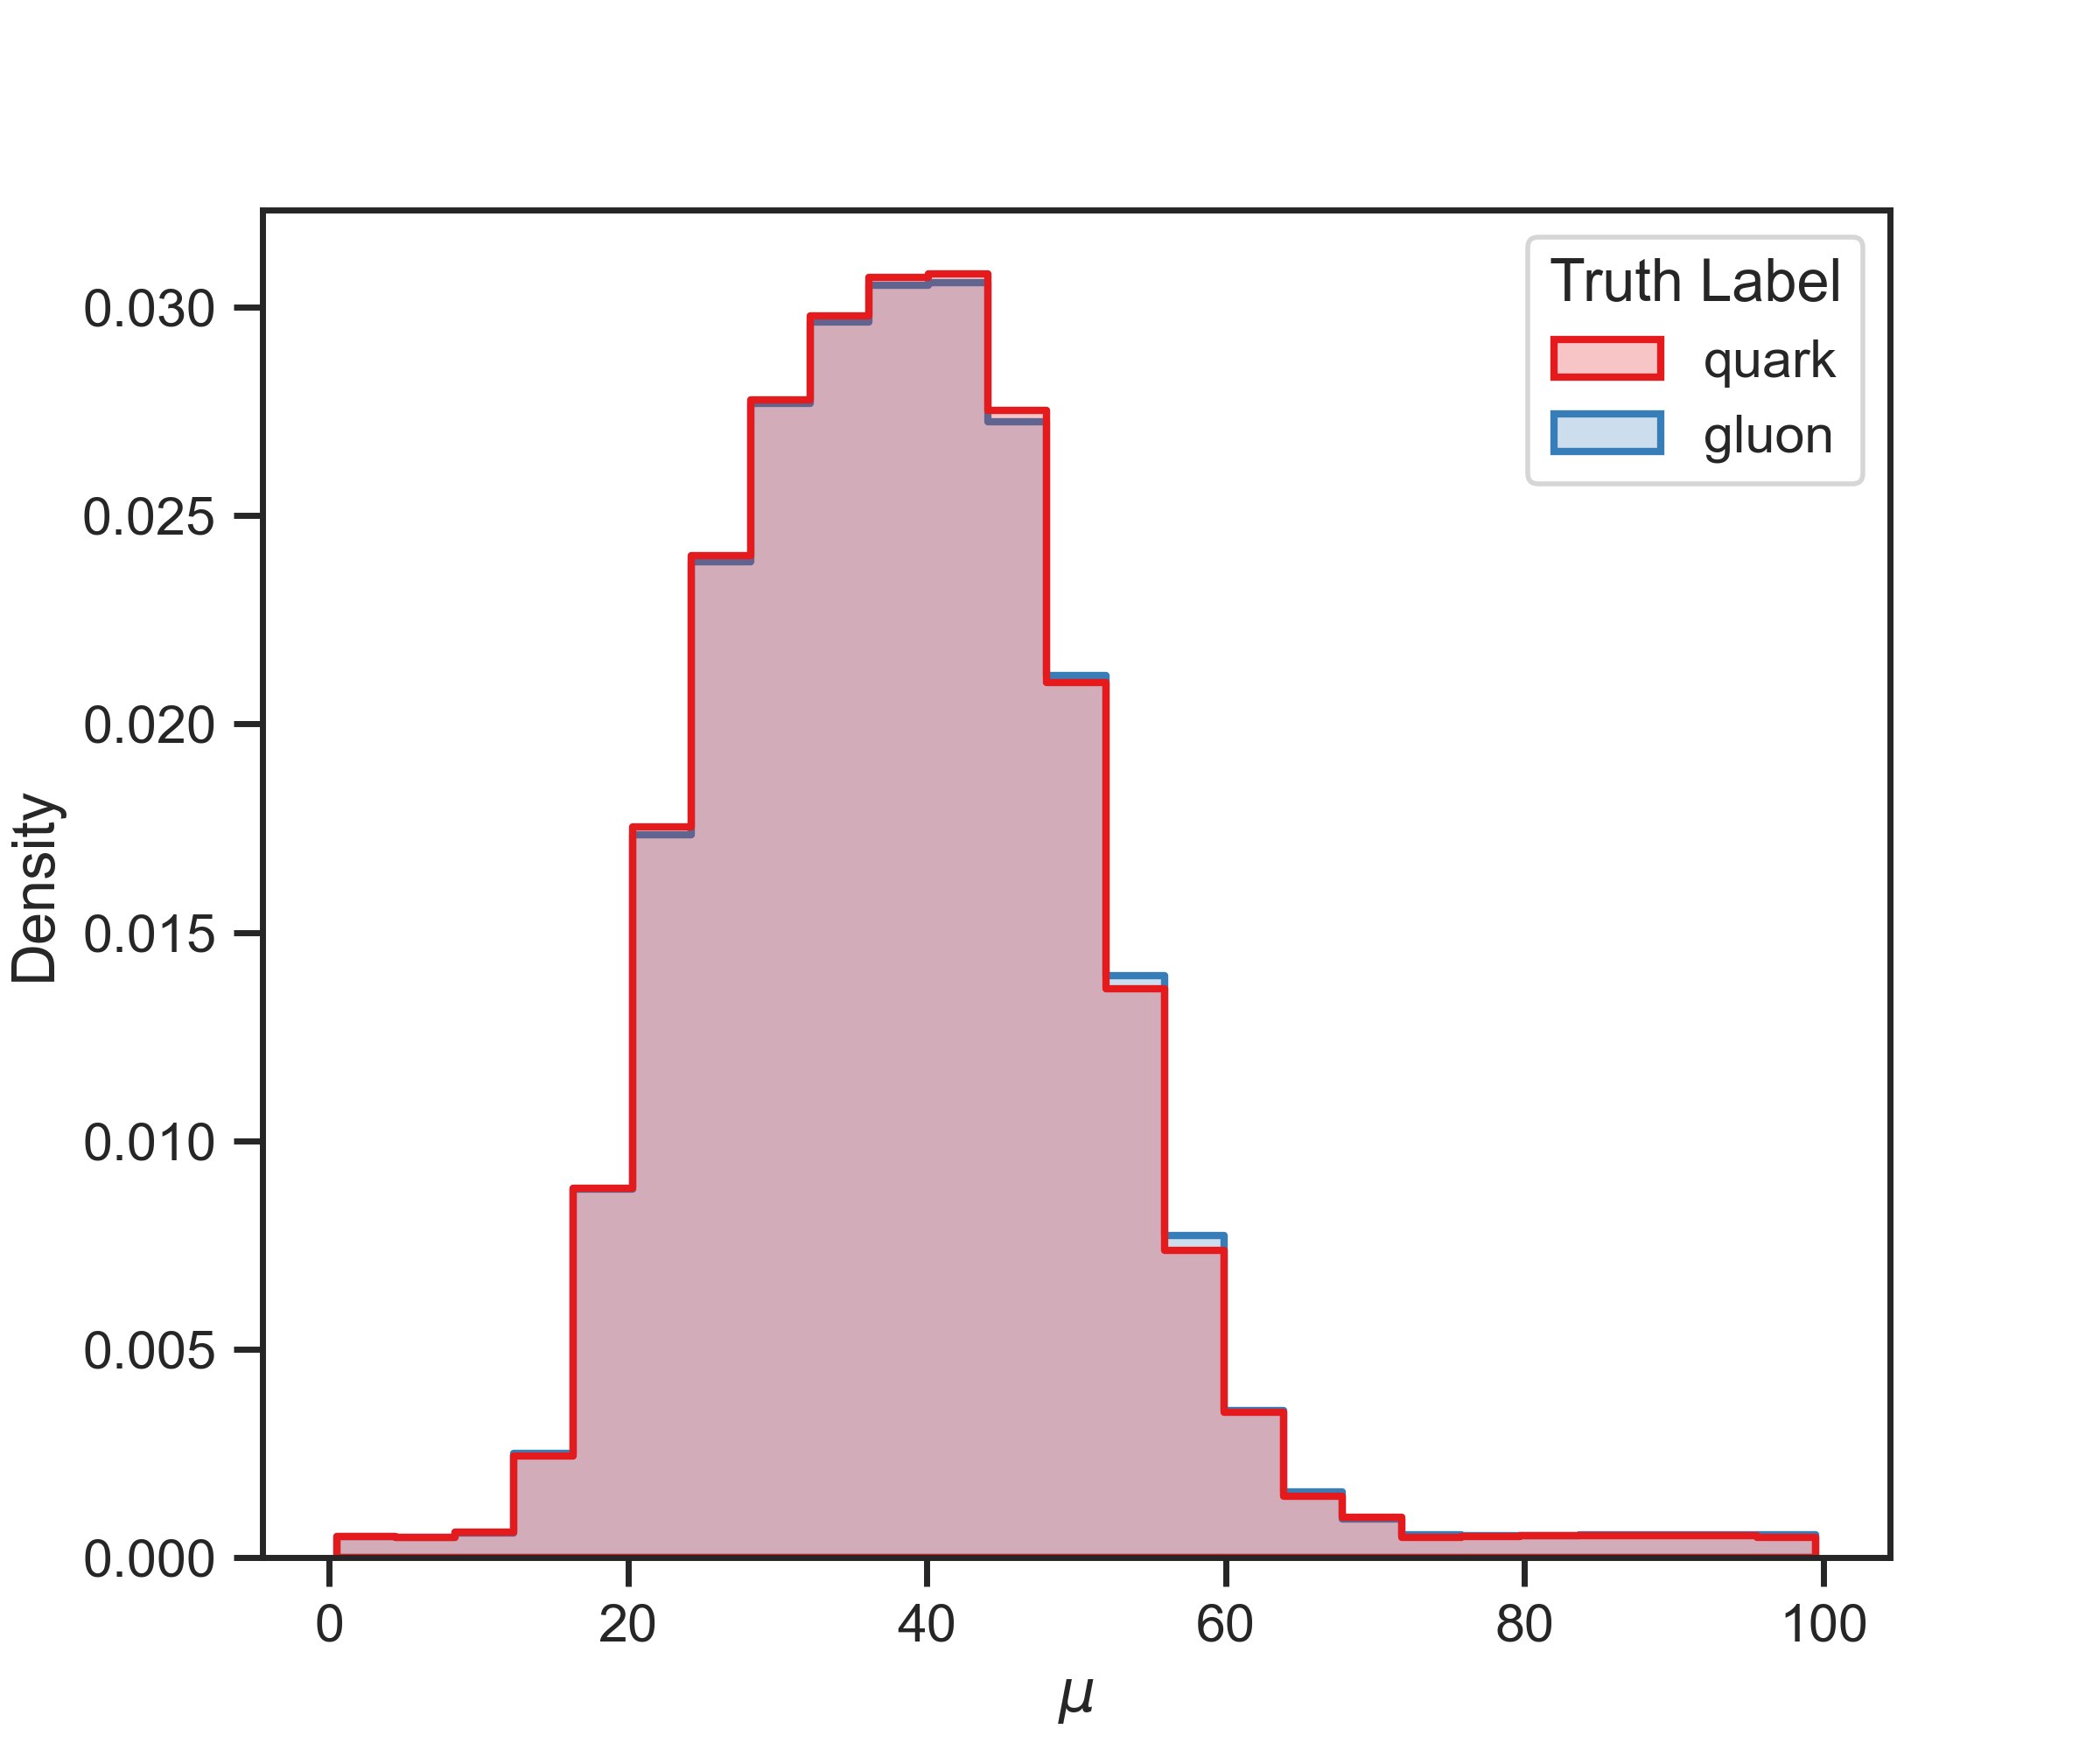
\includegraphics[width=1\textwidth]{src/plots/distributions/highlevel/corrected_averageInteractionsPerCrossing[0].png}
		\caption{\texttt{averageInteractionsPerCrossing[0]}}
		\label{fig:highlevel_0}
	\end{subfigure}
	\begin{subfigure}[t]{0.49\textwidth}
		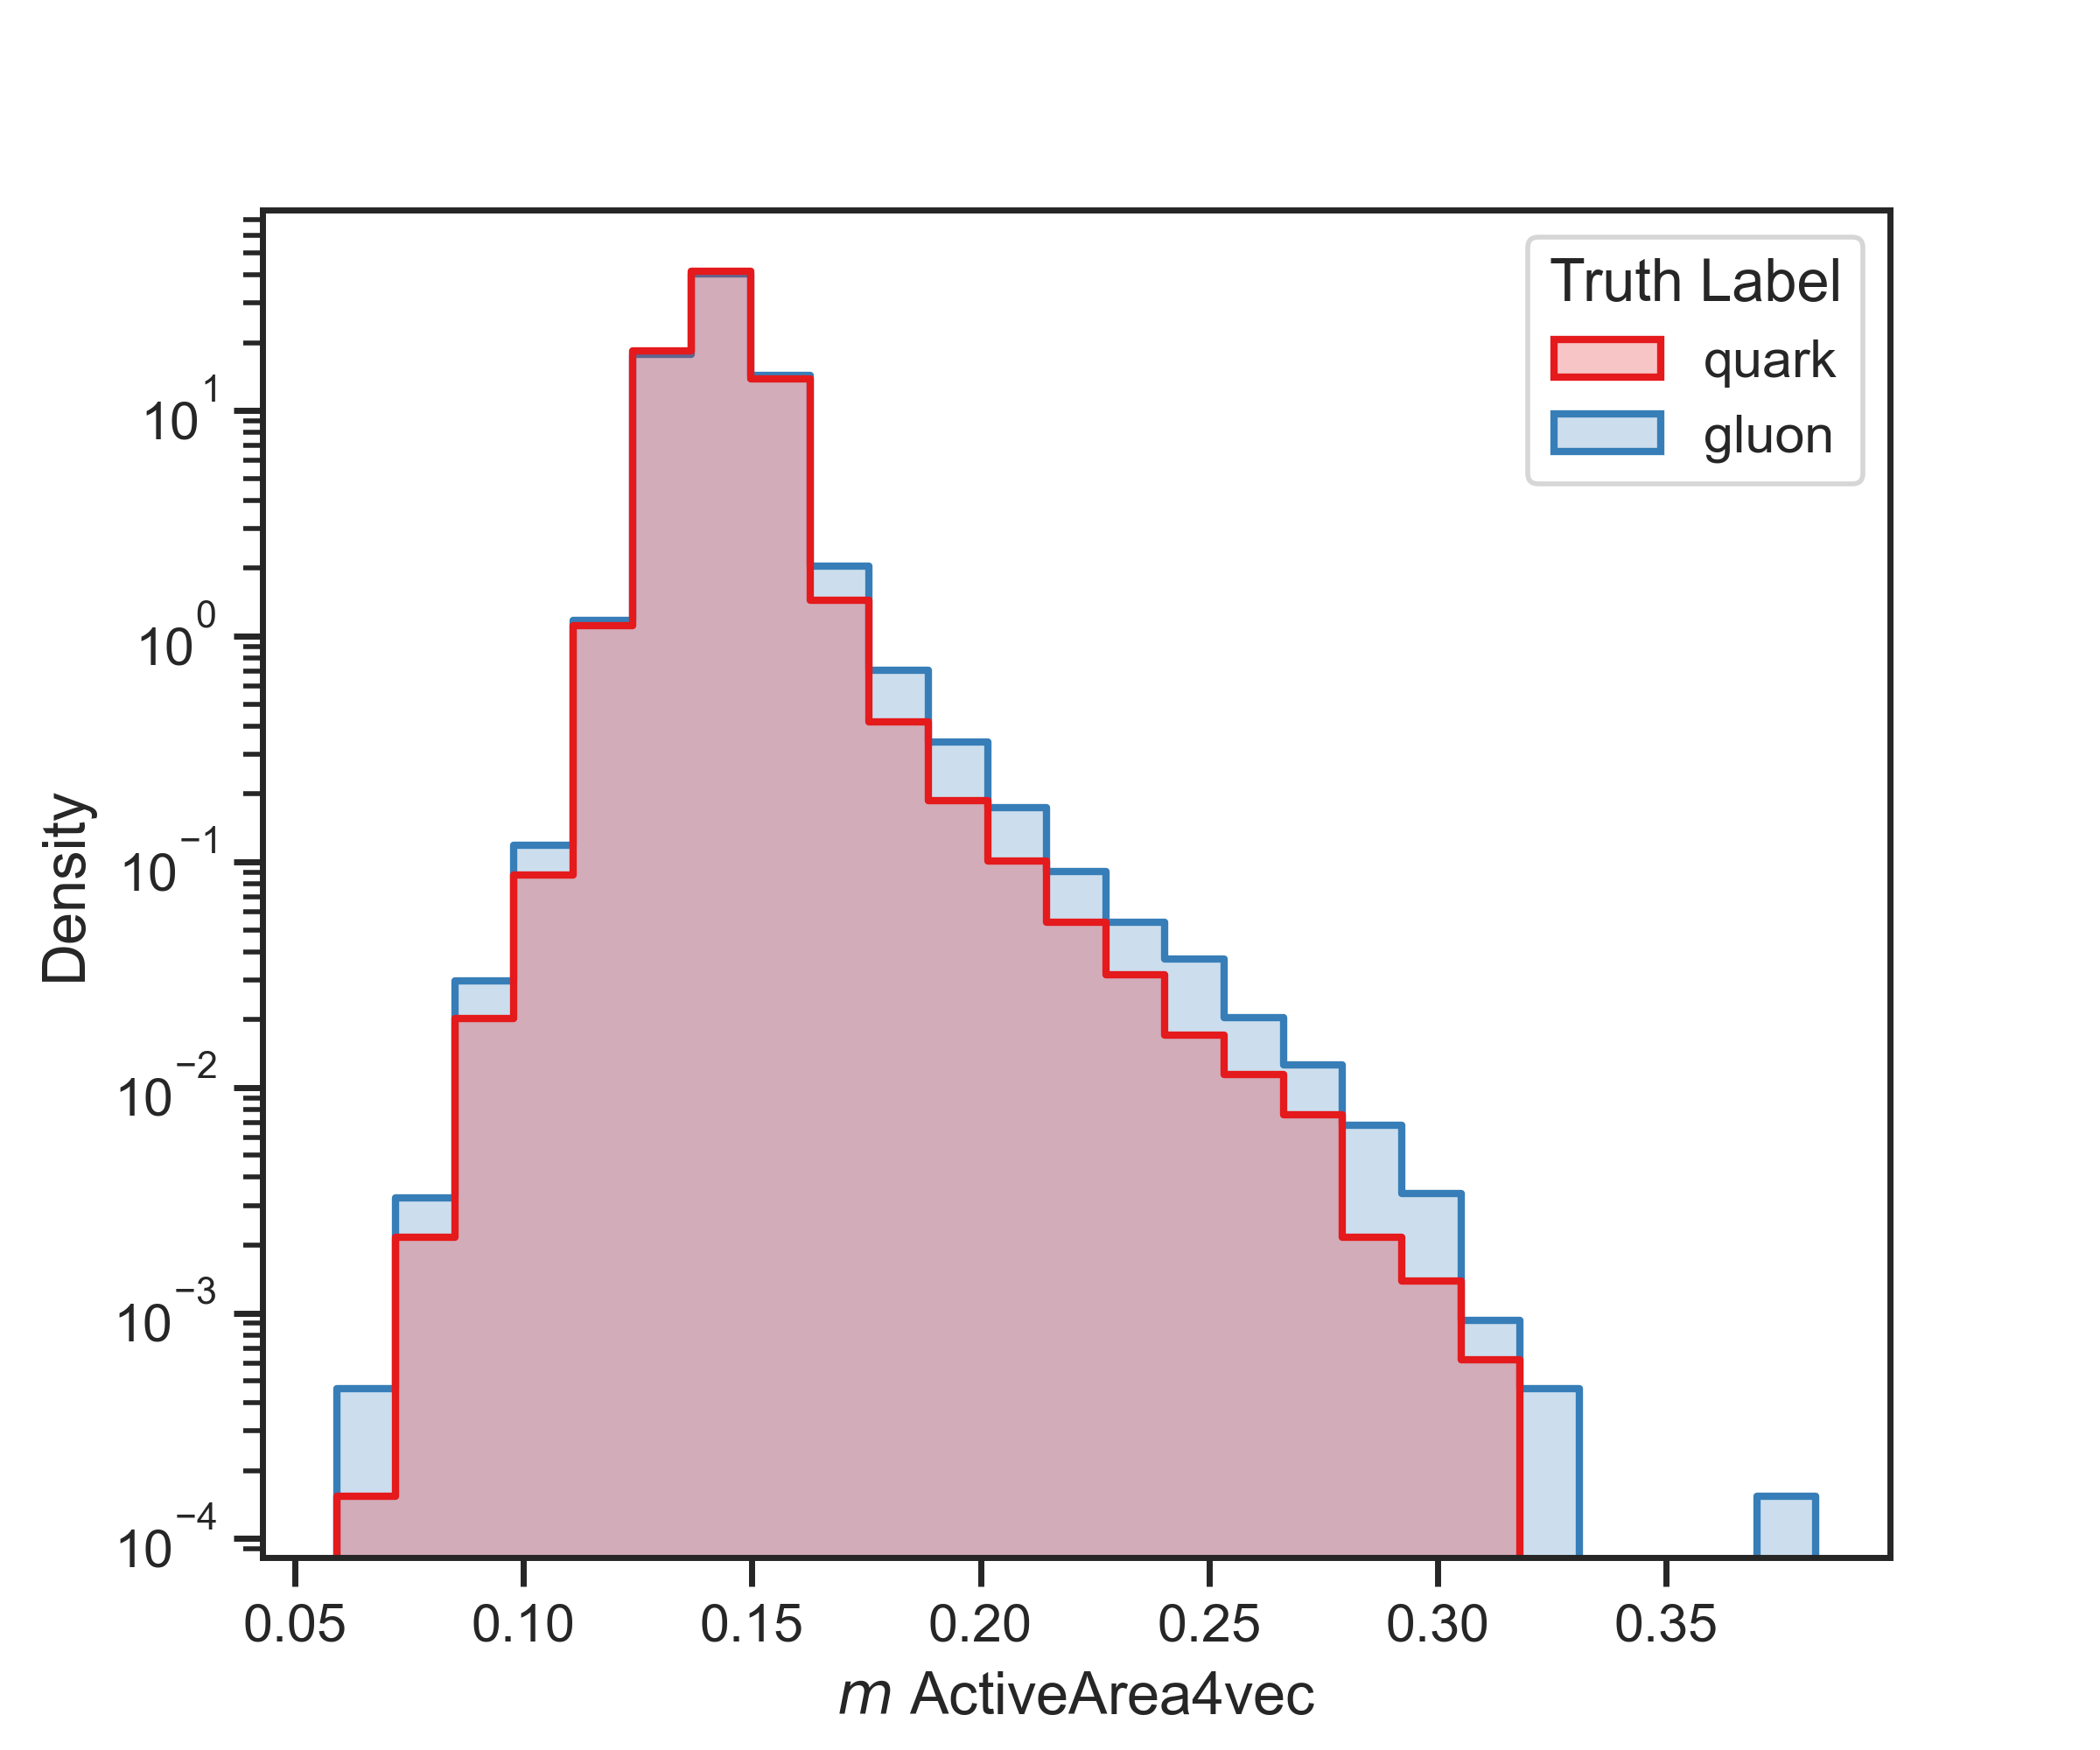
\includegraphics[width=1\textwidth]{src/plots/distributions/highlevel/jets_ActiveArea4vec_m.png}
		\caption{\texttt{jets\_ActiveArea4vec\_m}}
		\label{fig:highlevel_1}
	\end{subfigure}
	\begin{subfigure}[t]{0.49\textwidth}
		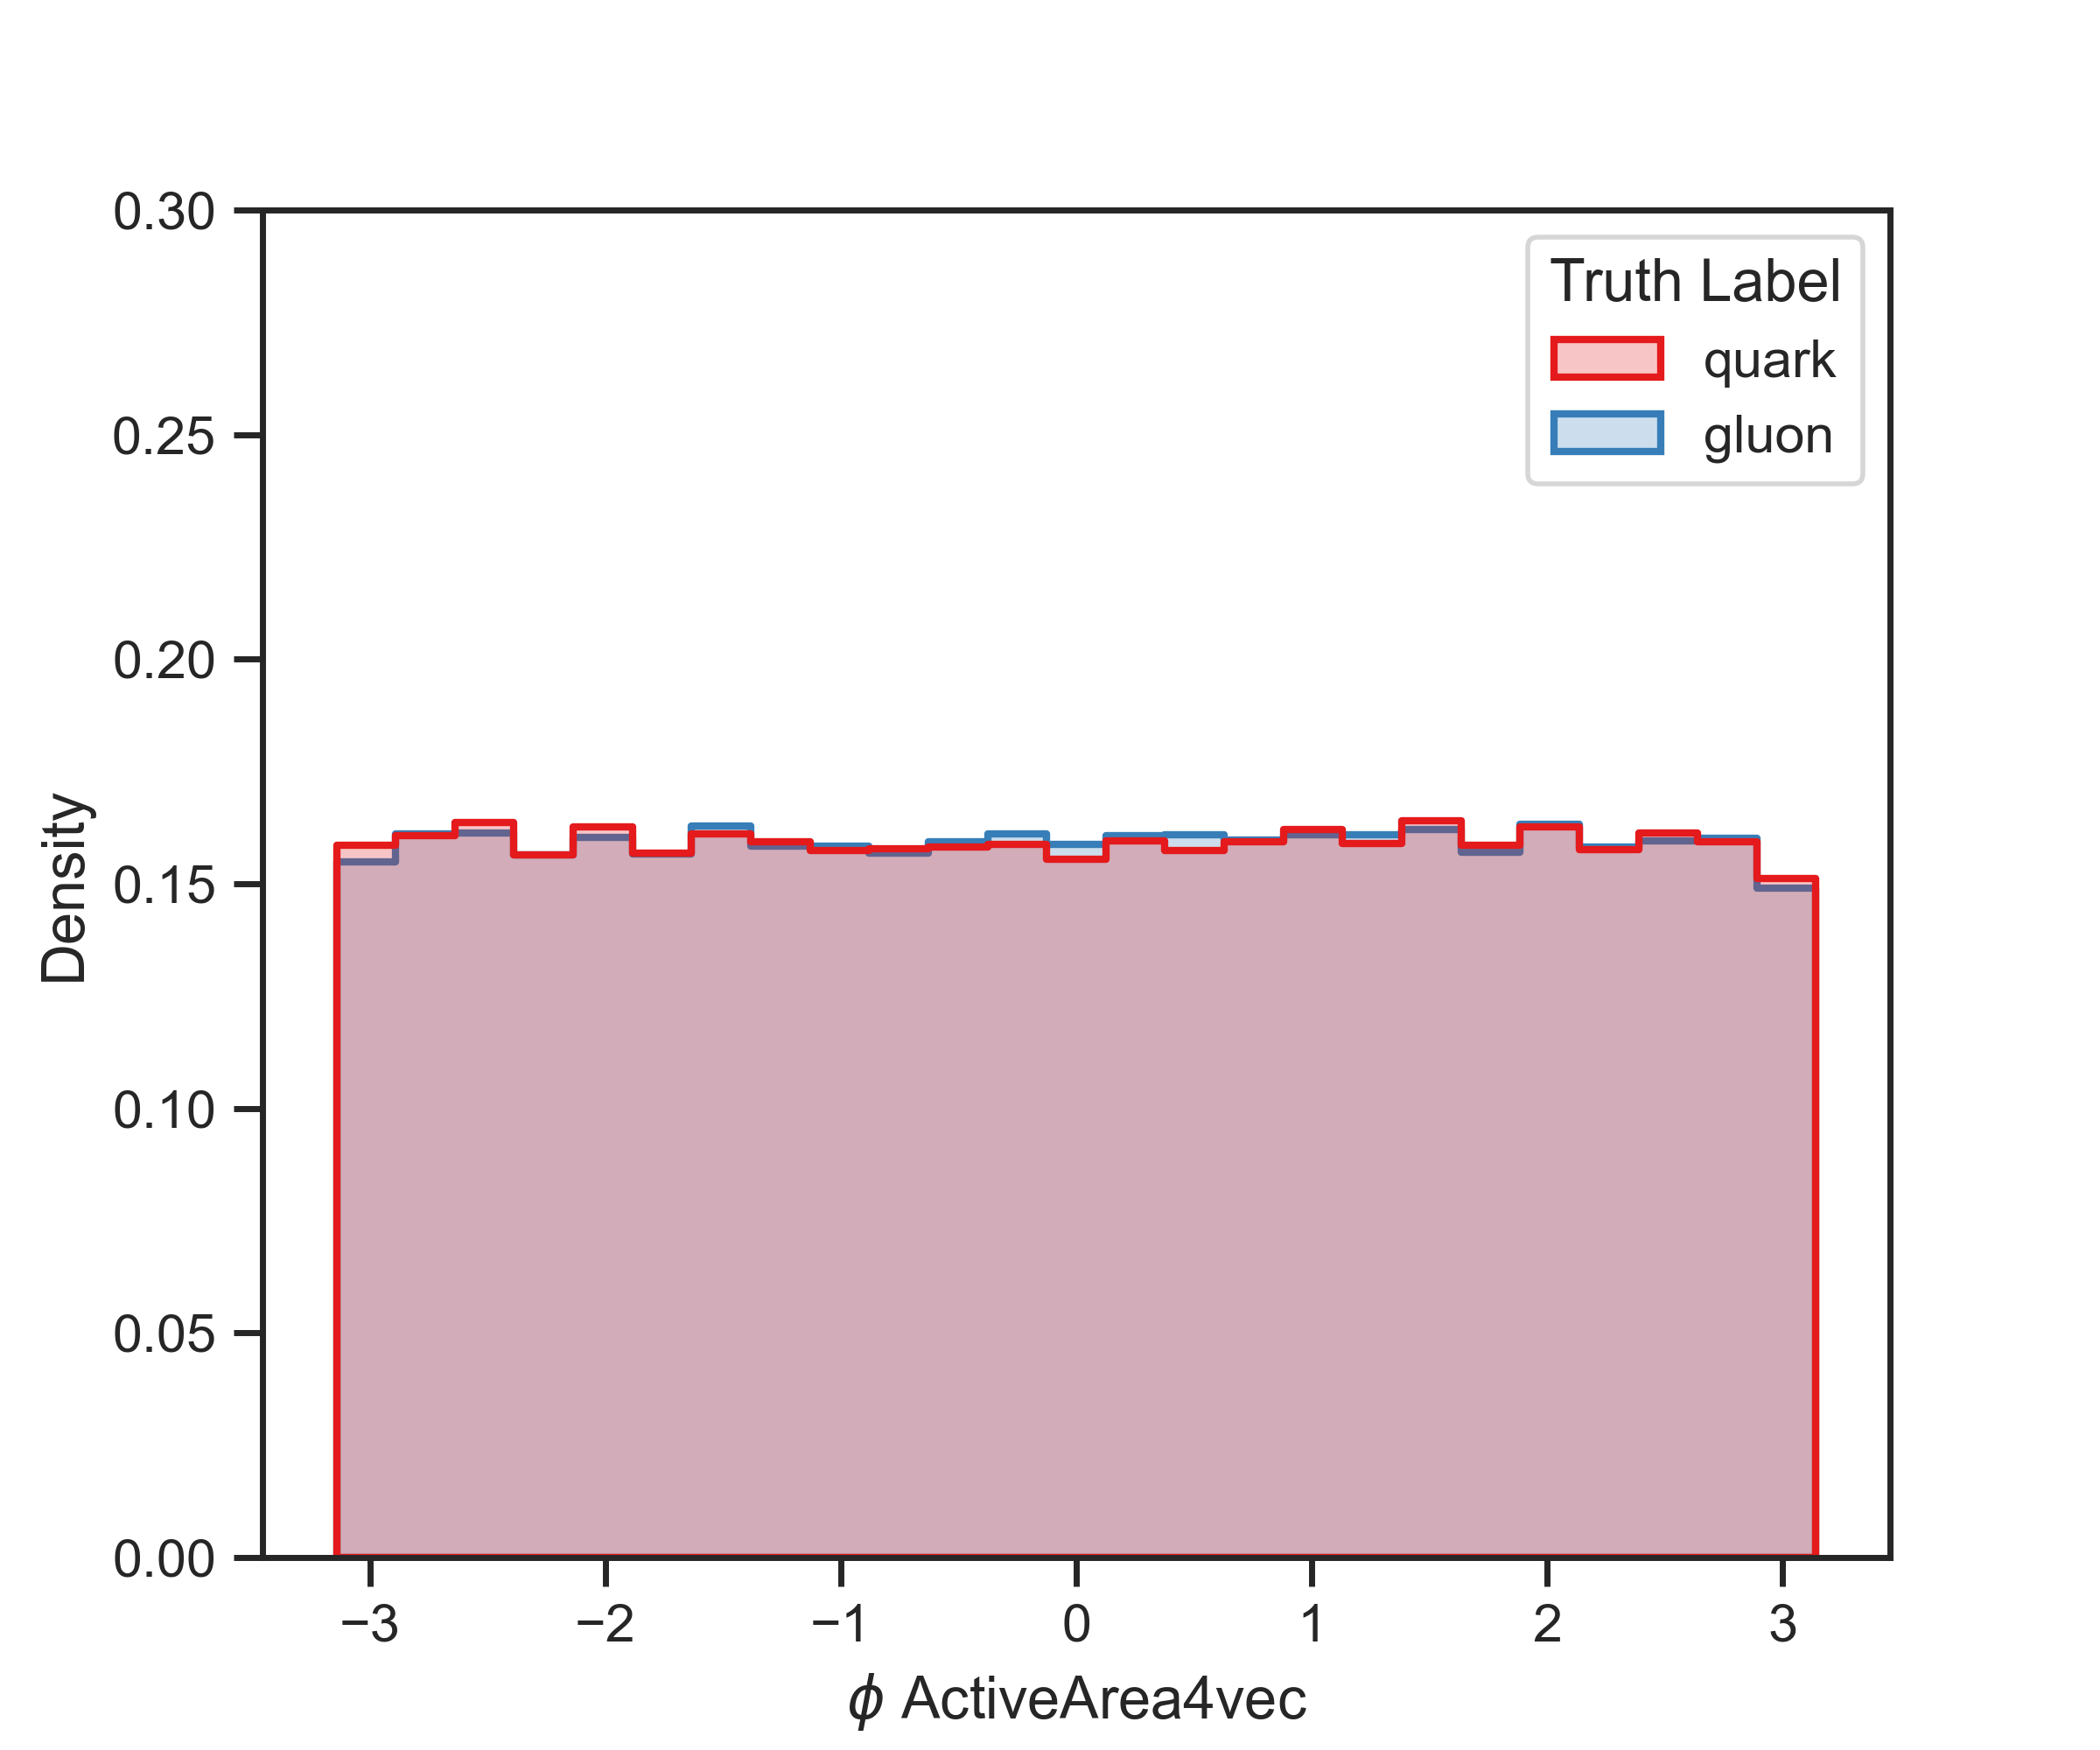
\includegraphics[width=1\textwidth]{src/plots/distributions/highlevel/jets_ActiveArea4vec_phi.png}
		\caption{\texttt{jets\_ActiveArea4vec\_phi}}
		\label{fig:highlevel_2}
	\end{subfigure}
	\begin{subfigure}[t]{0.49\textwidth}
		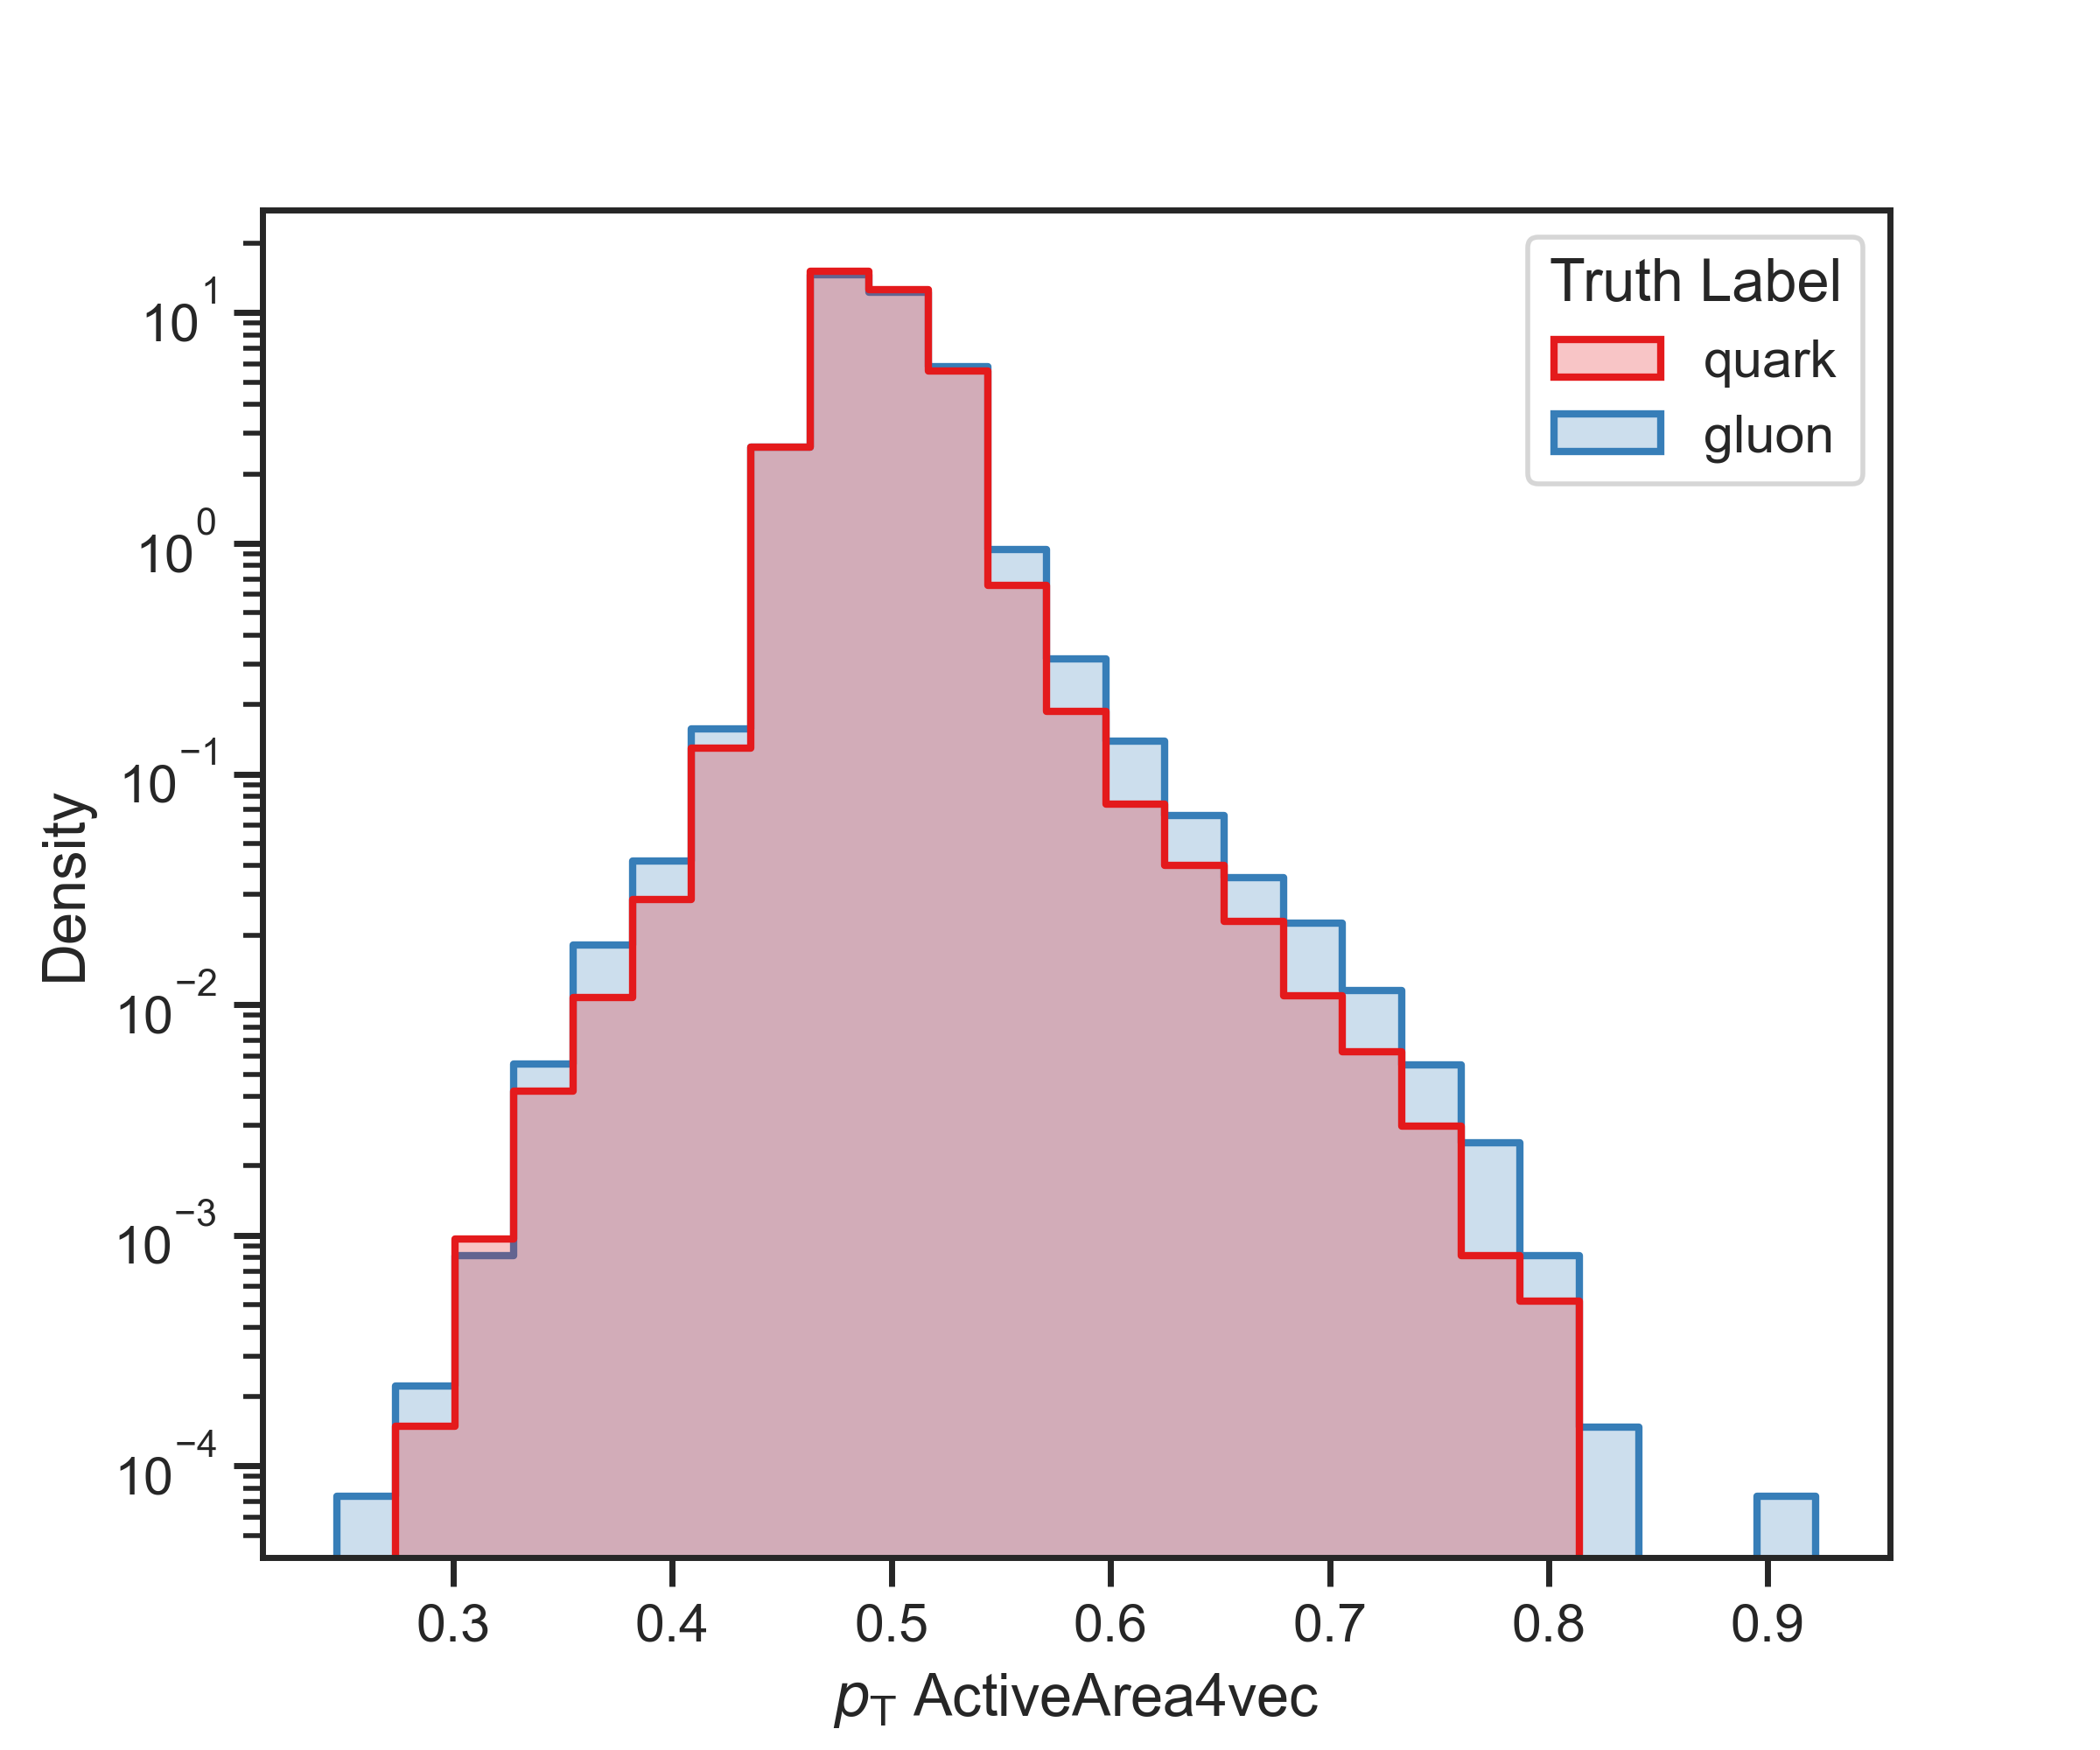
\includegraphics[width=1\textwidth]{src/plots/distributions/highlevel/jets_ActiveArea4vec_pt.png}
		\caption{\texttt{jets\_ActiveArea4vec\_pt}}
		\label{fig:highlevel_3}
	\end{subfigure}
	\begin{subfigure}[t]{0.49\textwidth}
		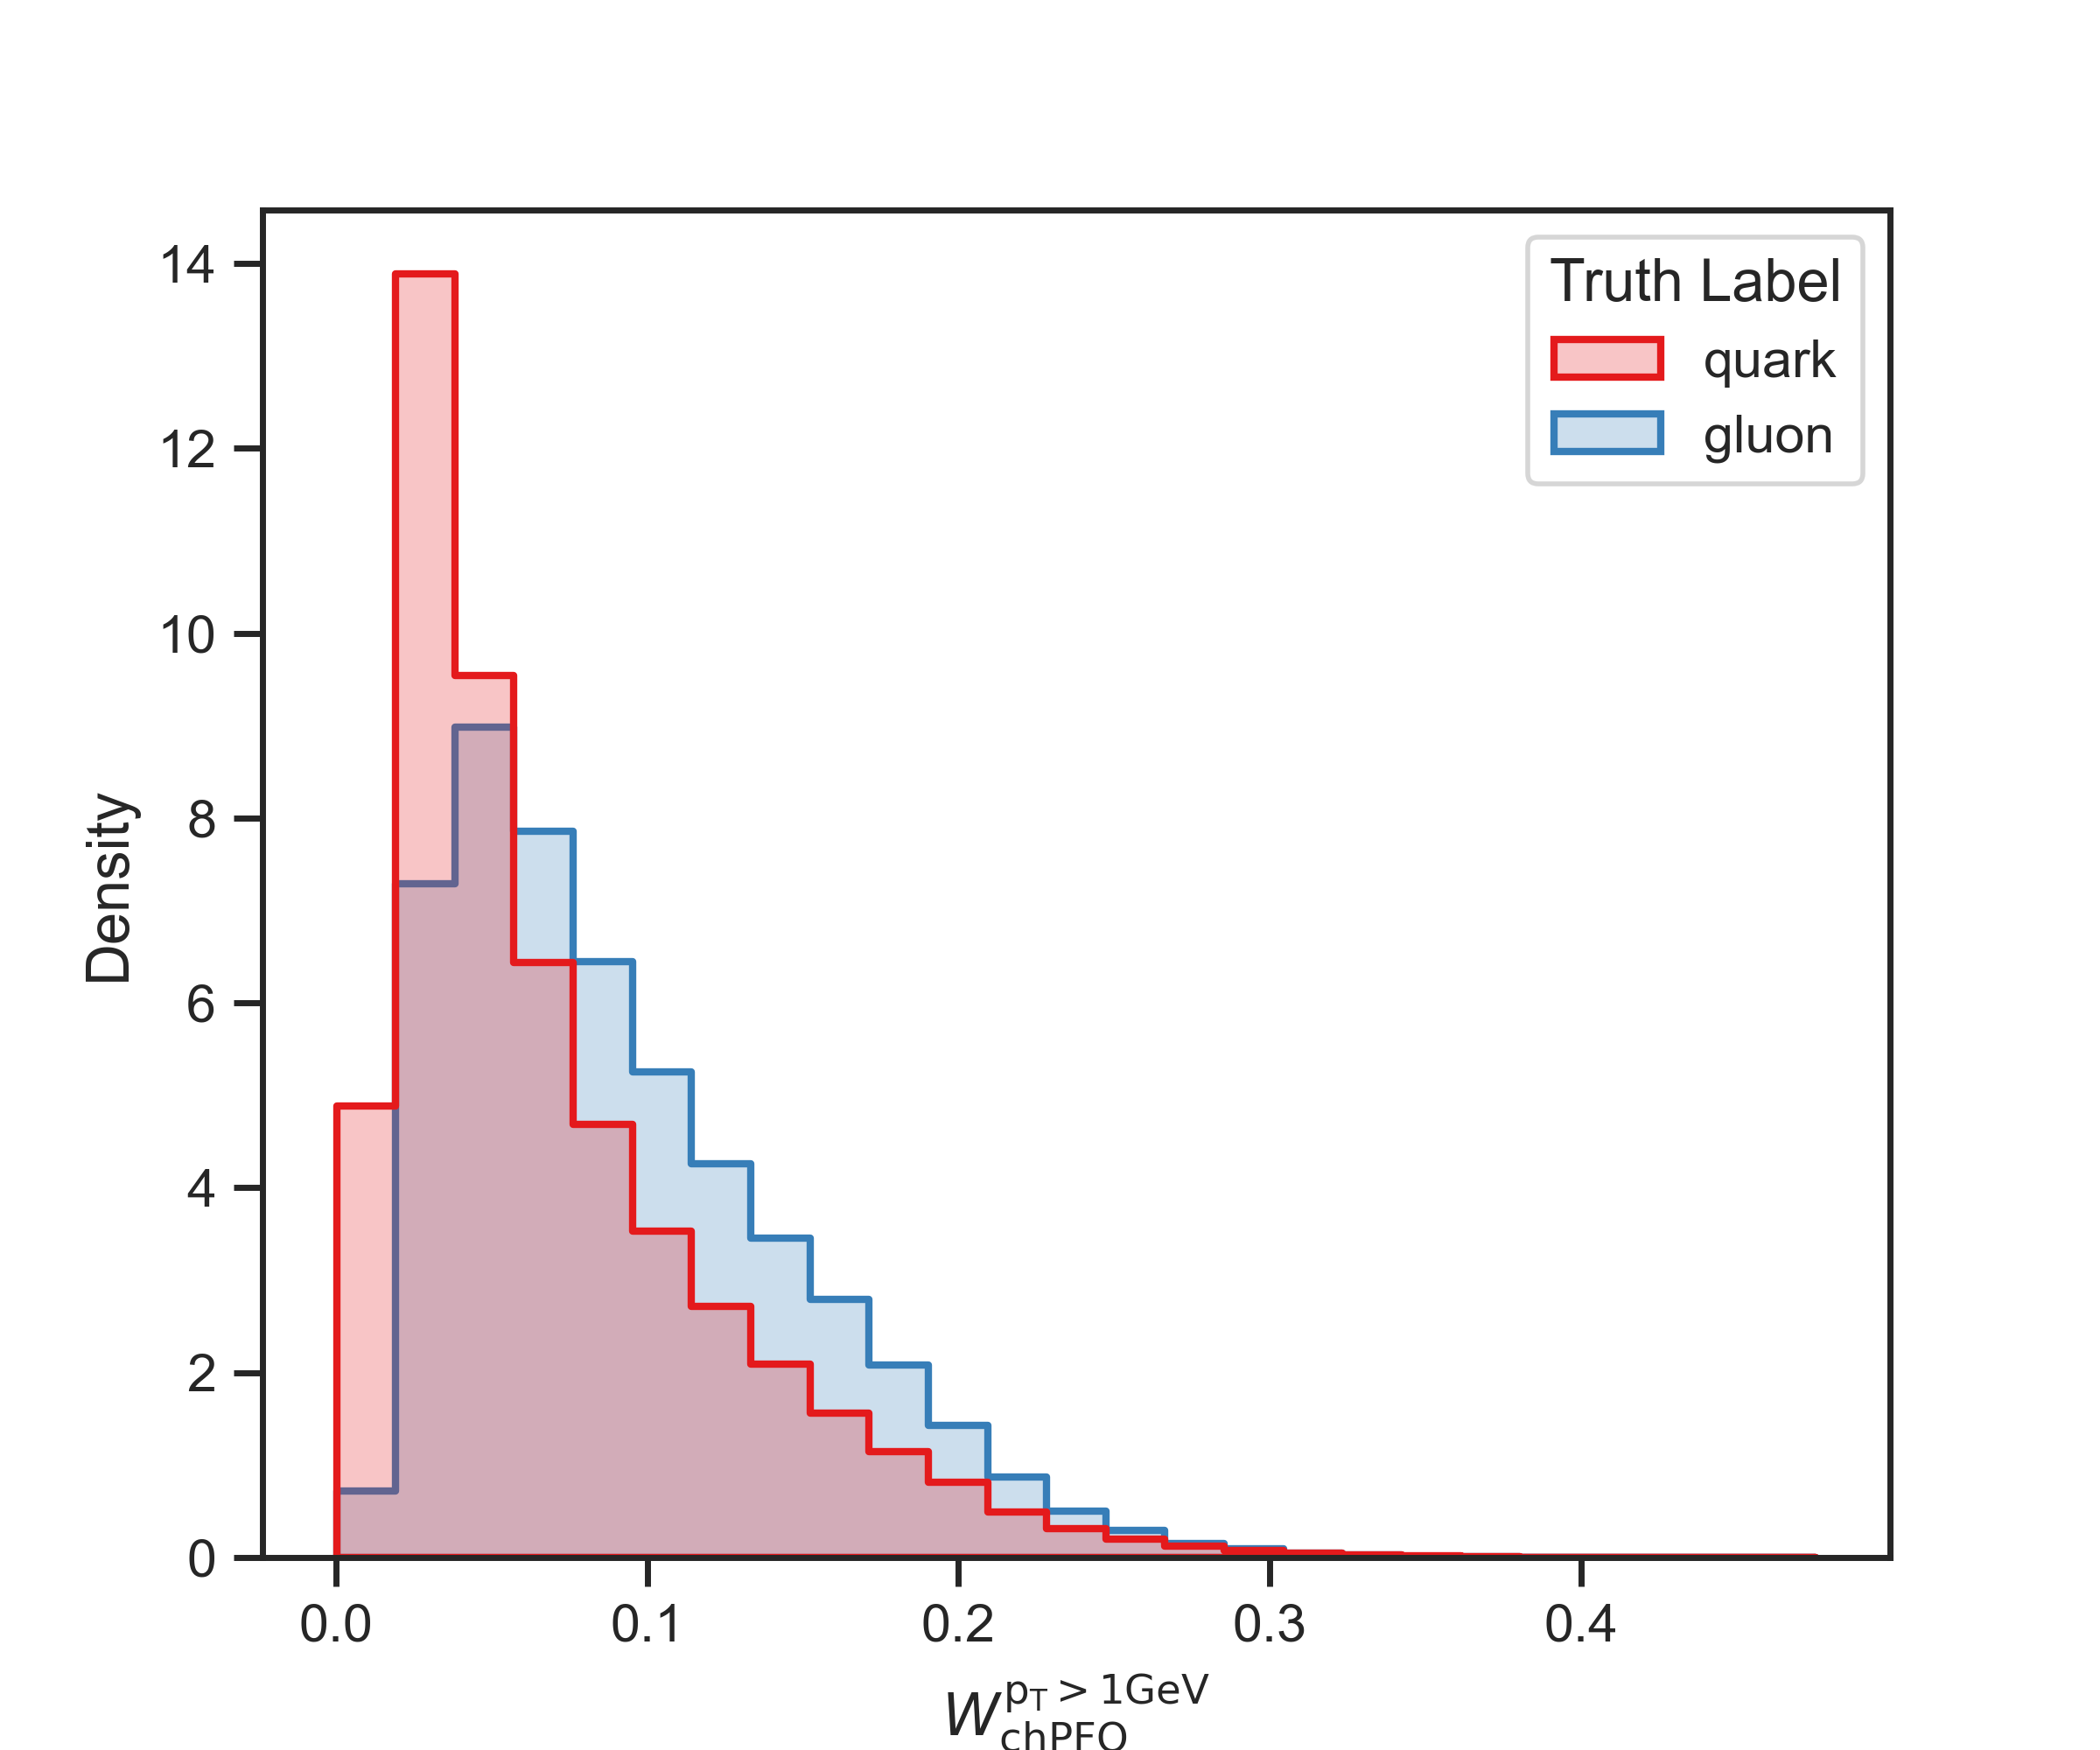
\includegraphics[width=1\textwidth]{src/plots/distributions/highlevel/jets_ChargedPFOWidthPt1000[0].png}
		\caption{\texttt{jets\_ChargedPFOWidthPt1000[0]}}
		\label{fig:highlevel_4}
	\end{subfigure}
	\begin{subfigure}[t]{0.49\textwidth}
		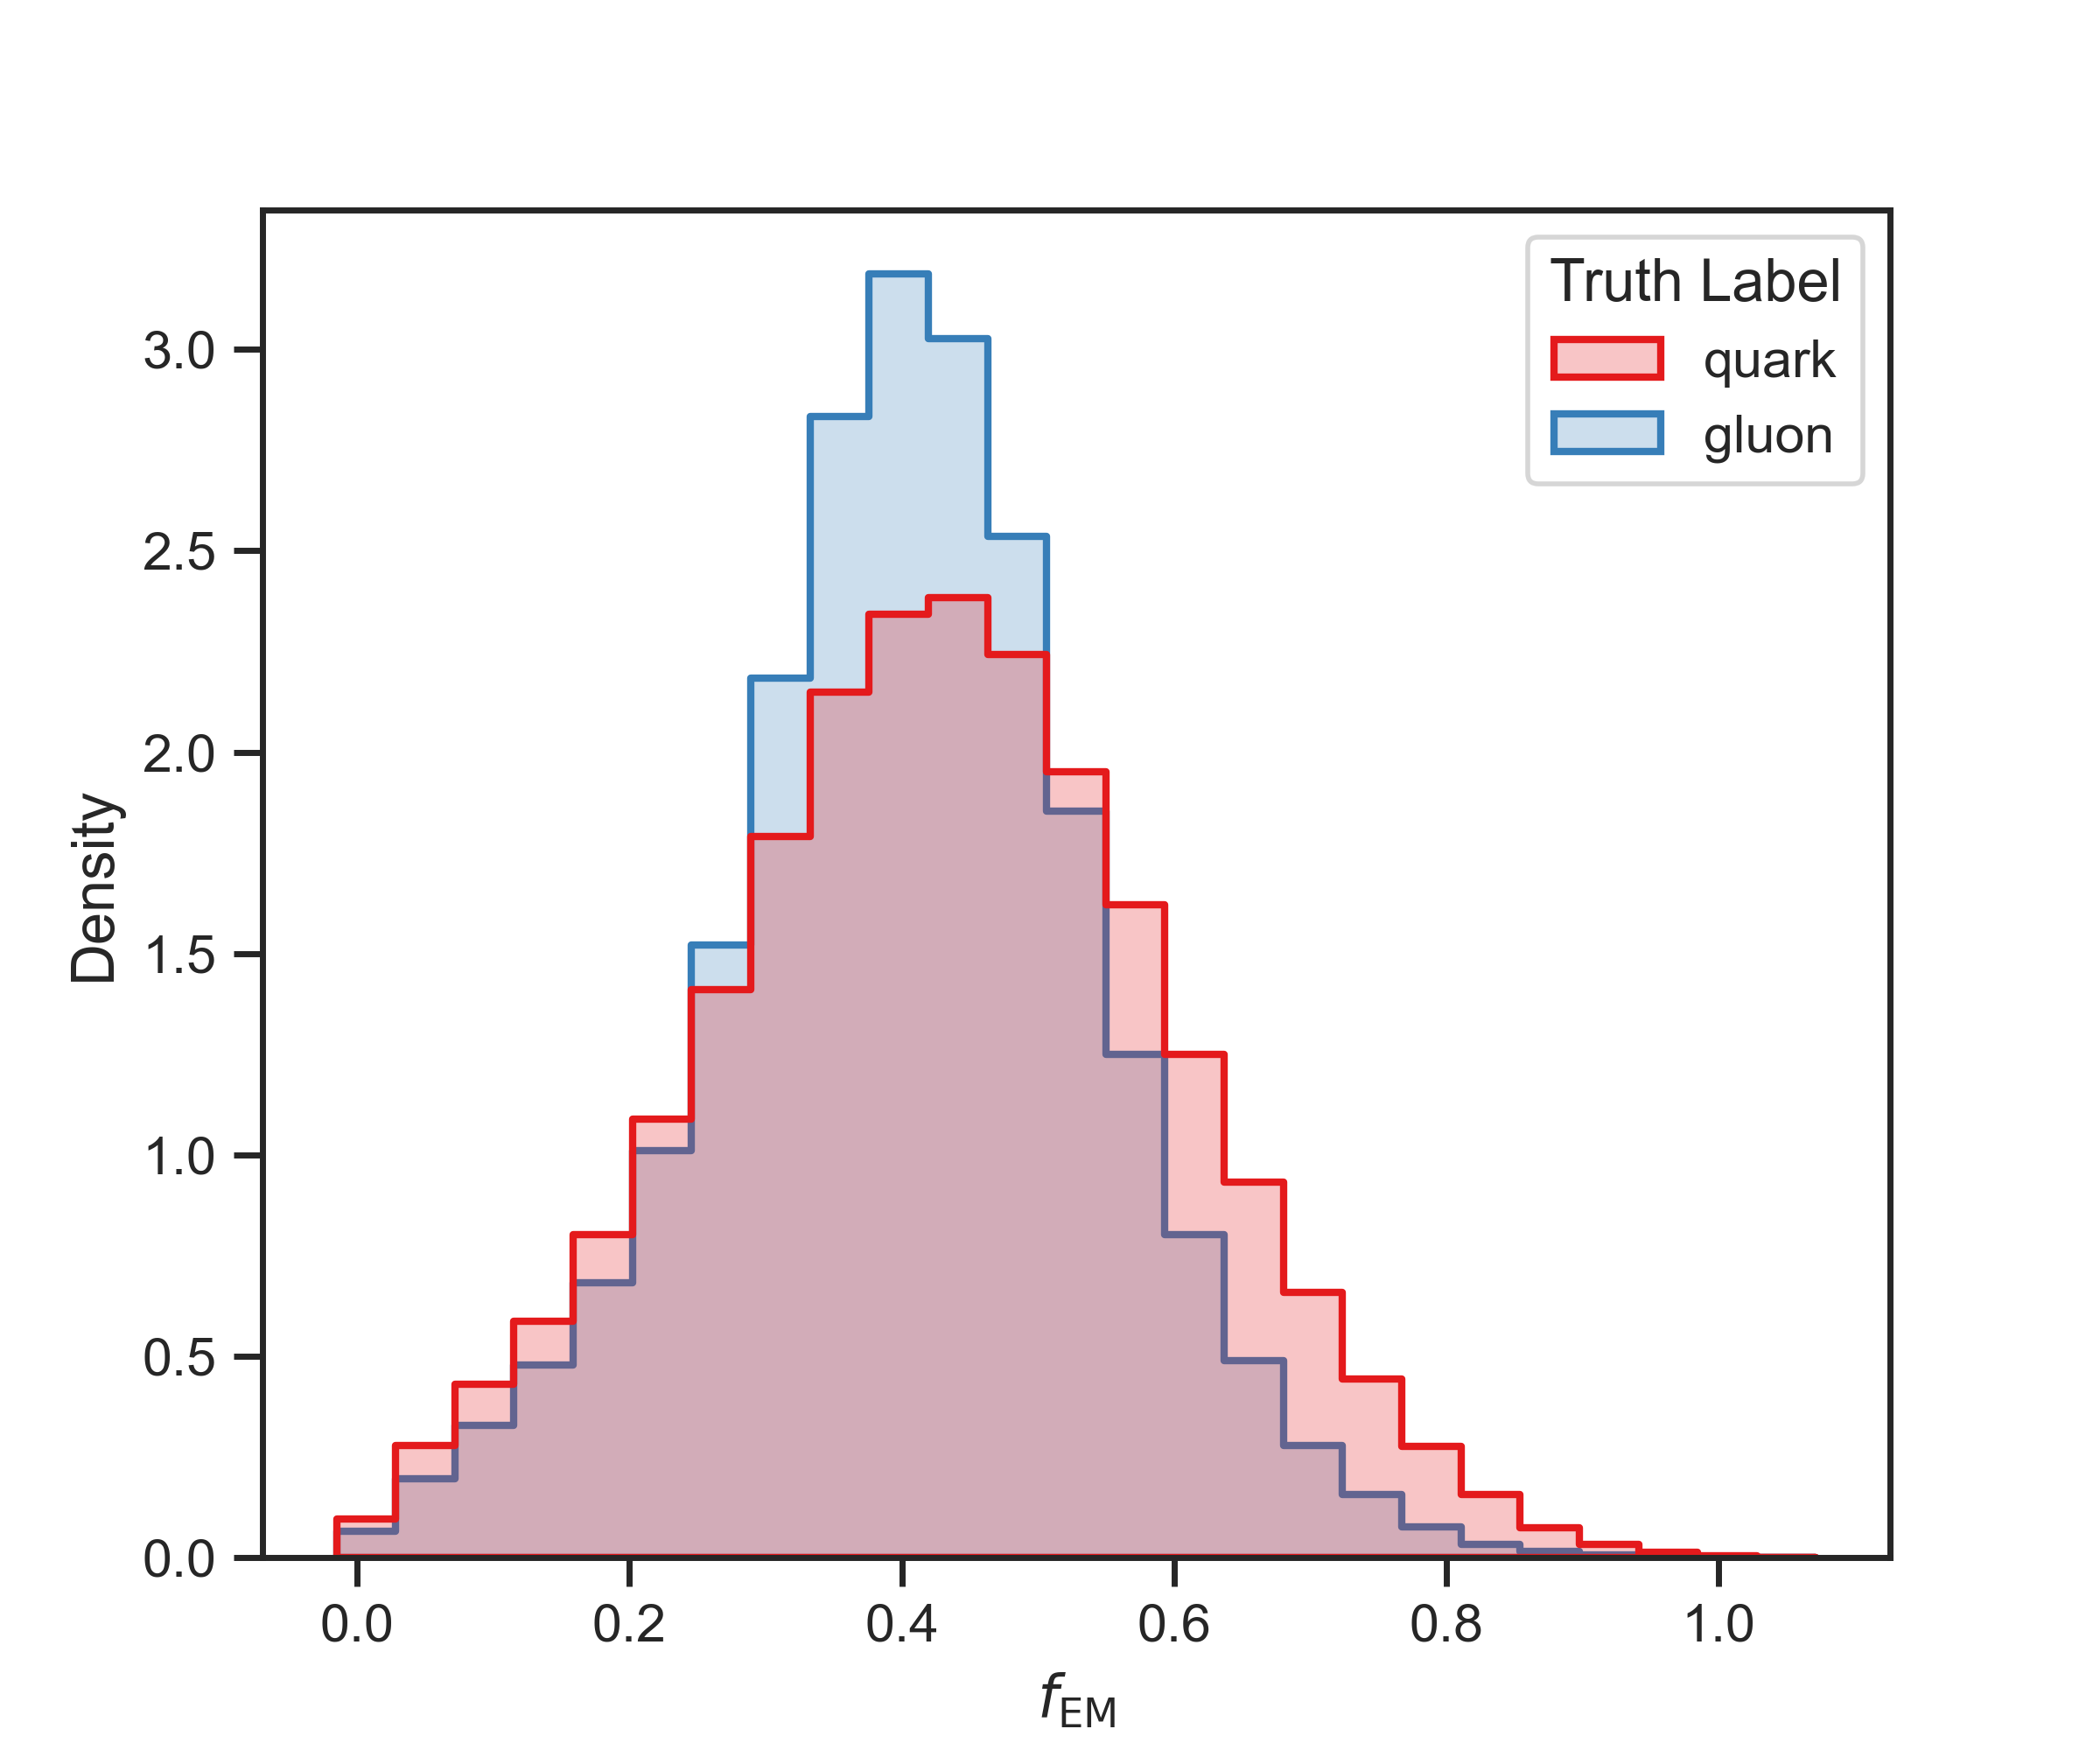
\includegraphics[width=1\textwidth]{src/plots/distributions/highlevel/jets_EMFrac.png}
		\caption{\texttt{jets\_EMFrac}}
		\label{fig:highlevel_5}
	\end{subfigure}
\caption{High-level Jet Variables, part 1}
\label{fig:highlevel_0-5}
\end{figure}

\begin{figure}[!htb]
	\centering
	\begin{subfigure}[t]{0.49\textwidth}
		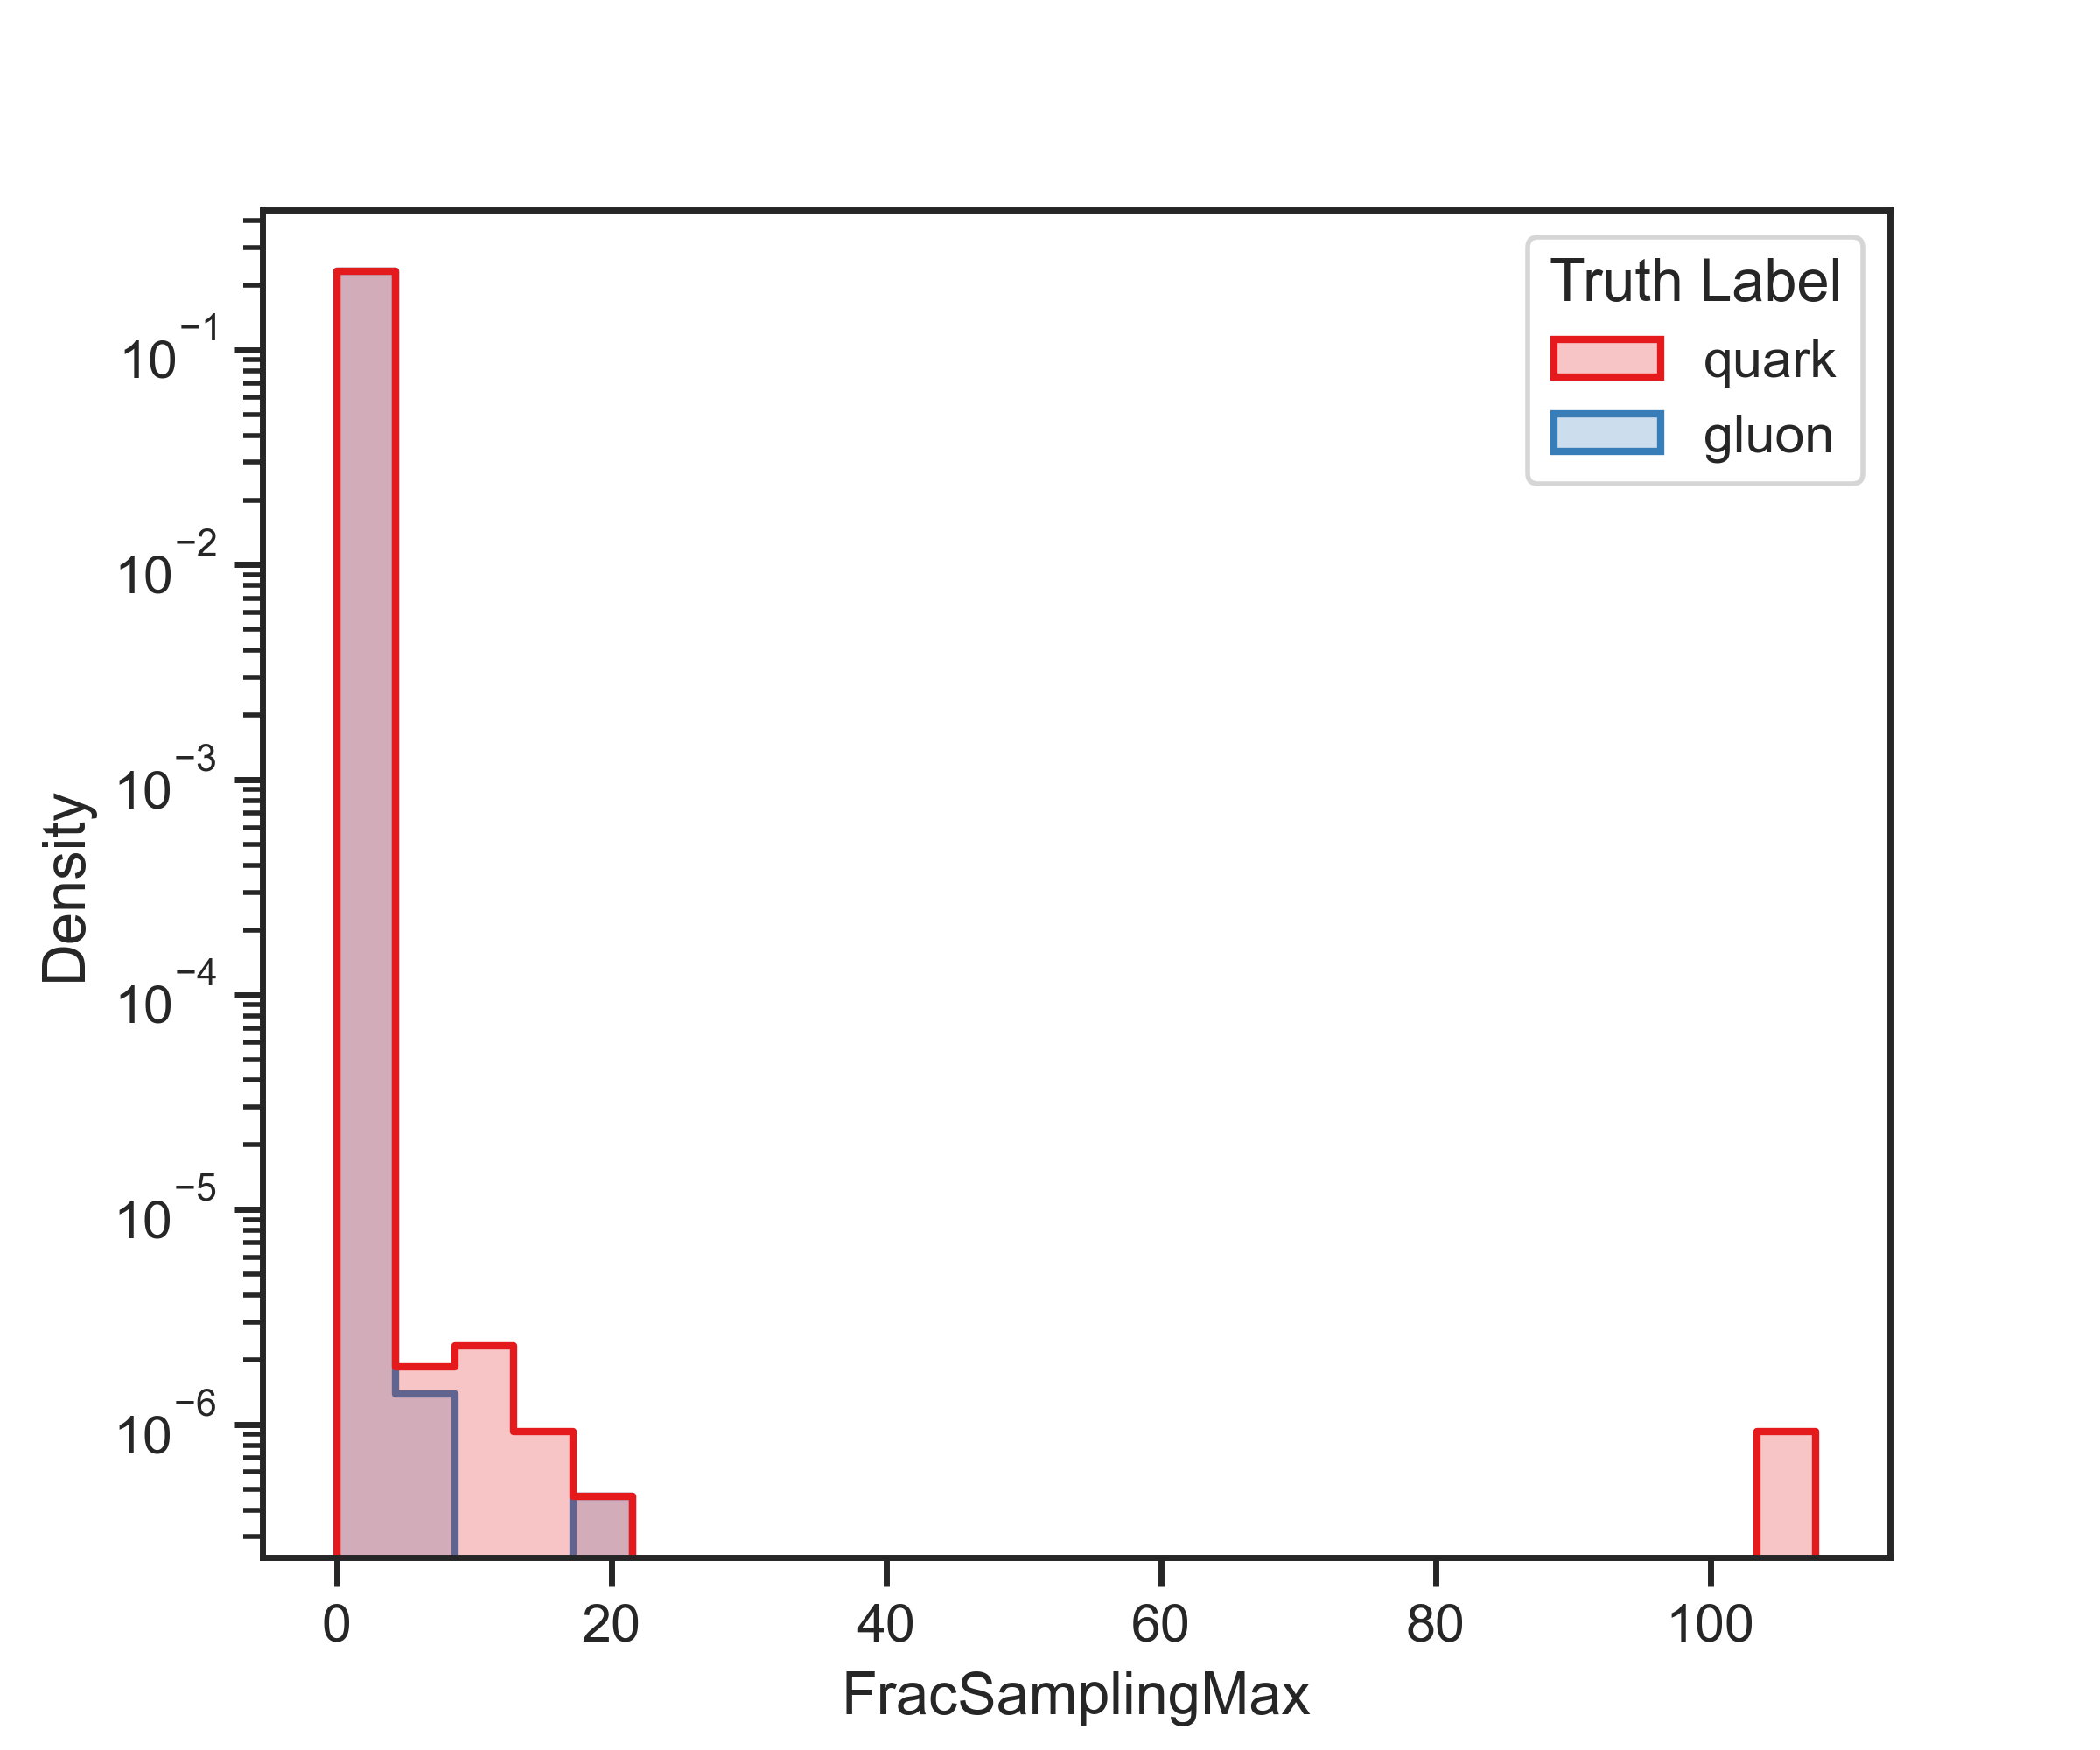
\includegraphics[width=1\textwidth]{src/plots/distributions/highlevel/jets_FracSamplingMax.png}
		\caption{\texttt{jets\_FracSamplingMax}}
		\label{fig:highlevel_6}
	\end{subfigure}
	\begin{subfigure}[t]{0.49\textwidth}
		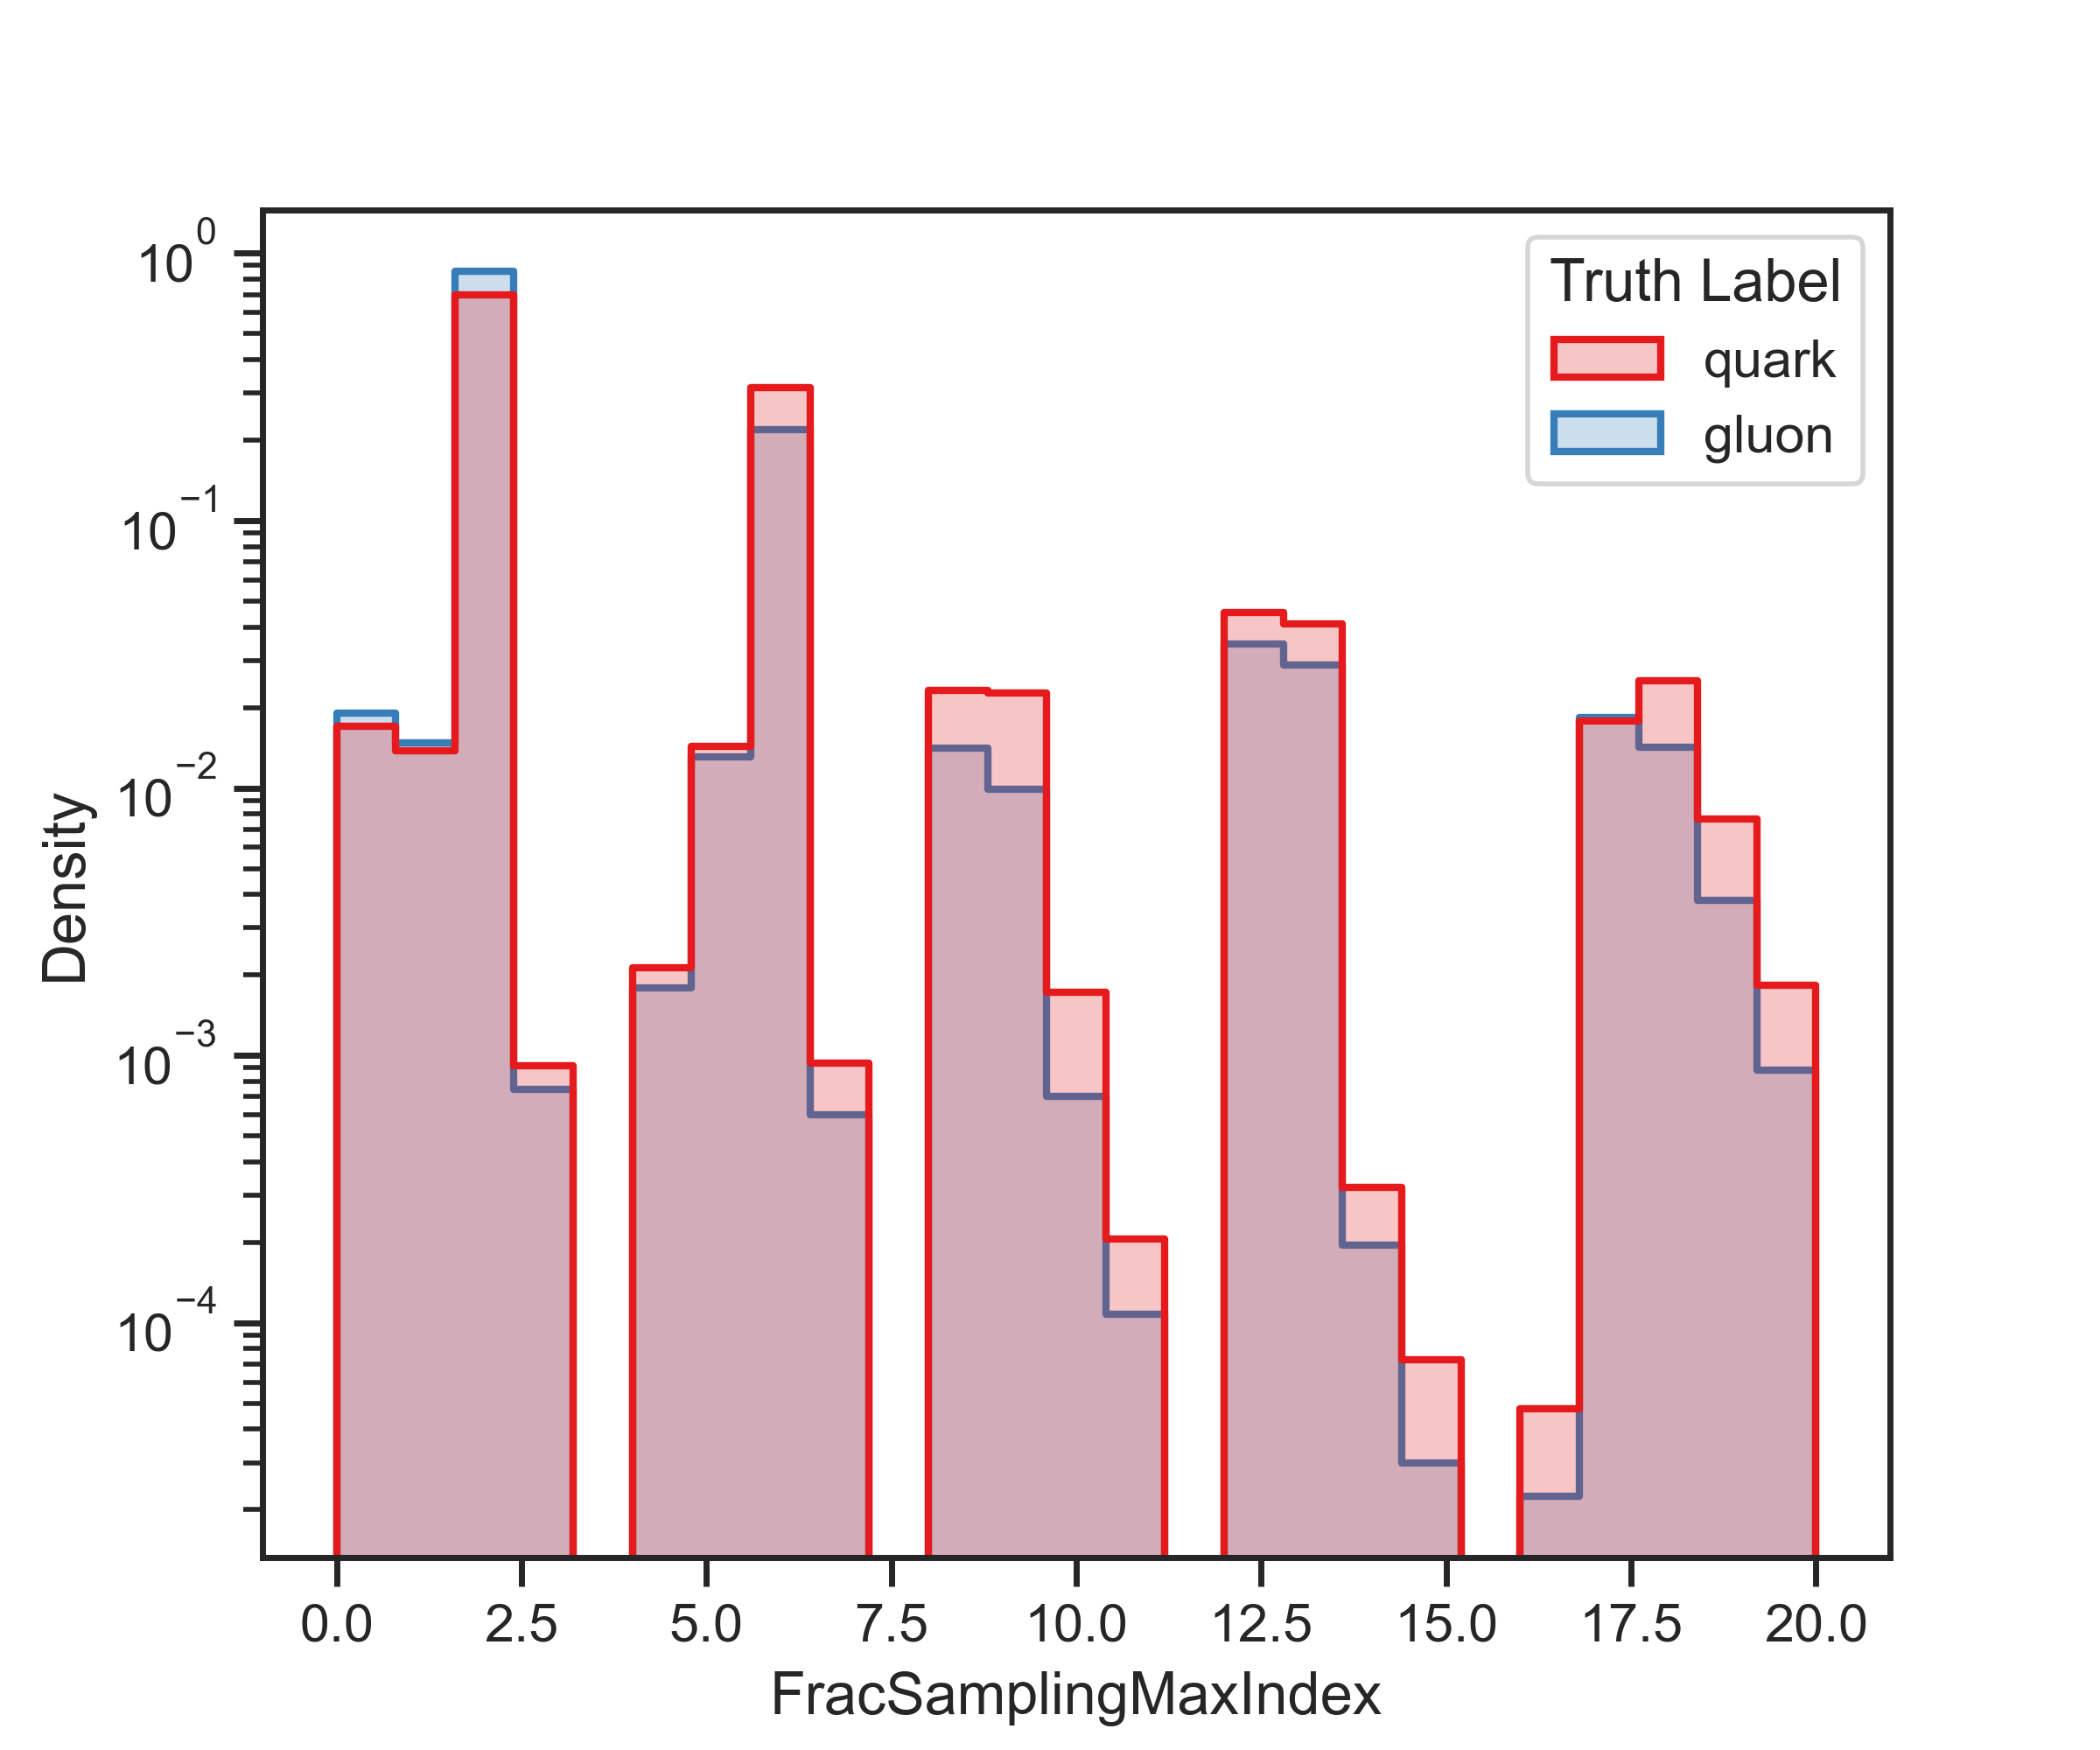
\includegraphics[width=1\textwidth]{src/plots/distributions/highlevel/jets_FracSamplingMaxIndex.png}
		\caption{\texttt{jets\_FracSamplingMaxIndex}}
		\label{fig:highlevel_7}
	\end{subfigure}
	\begin{subfigure}[t]{0.49\textwidth}
		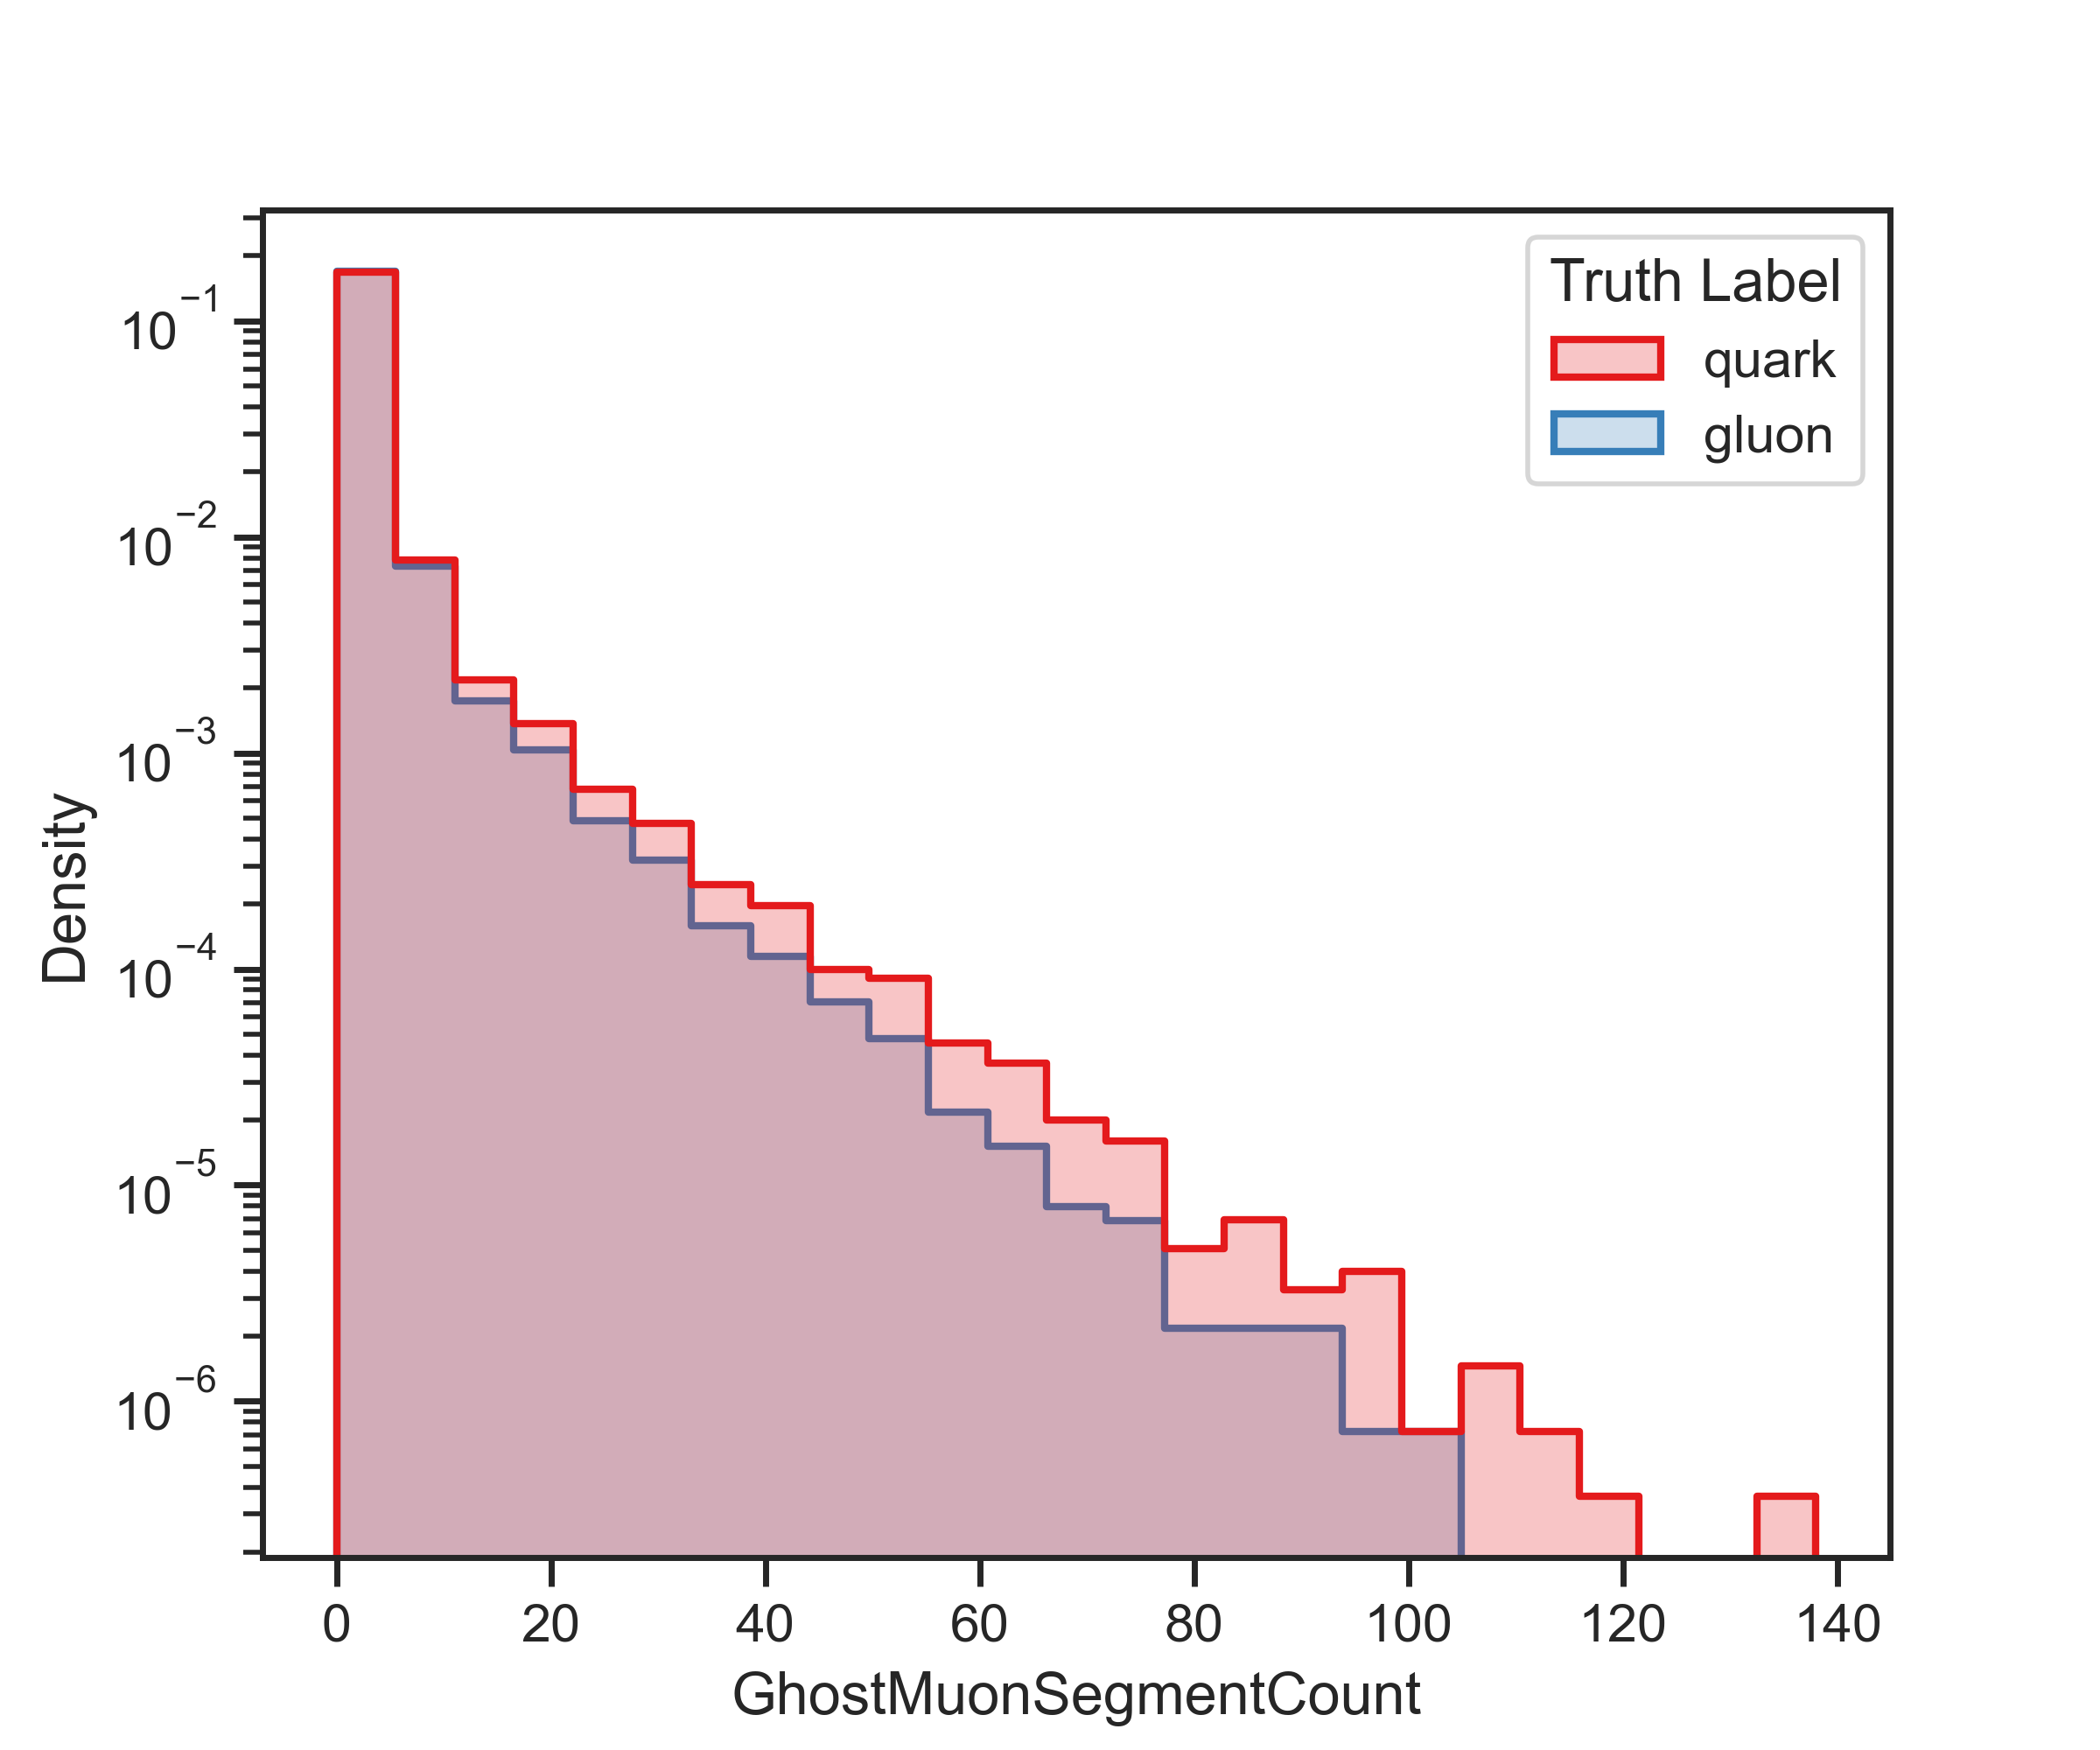
\includegraphics[width=1\textwidth]{src/plots/distributions/highlevel/jets_GhostMuonSegmentCount.png}
		\caption{\texttt{jets\_GhostMuonSegmentCount}}
		\label{fig:highlevel_8}
	\end{subfigure}
	\begin{subfigure}[t]{0.49\textwidth}
		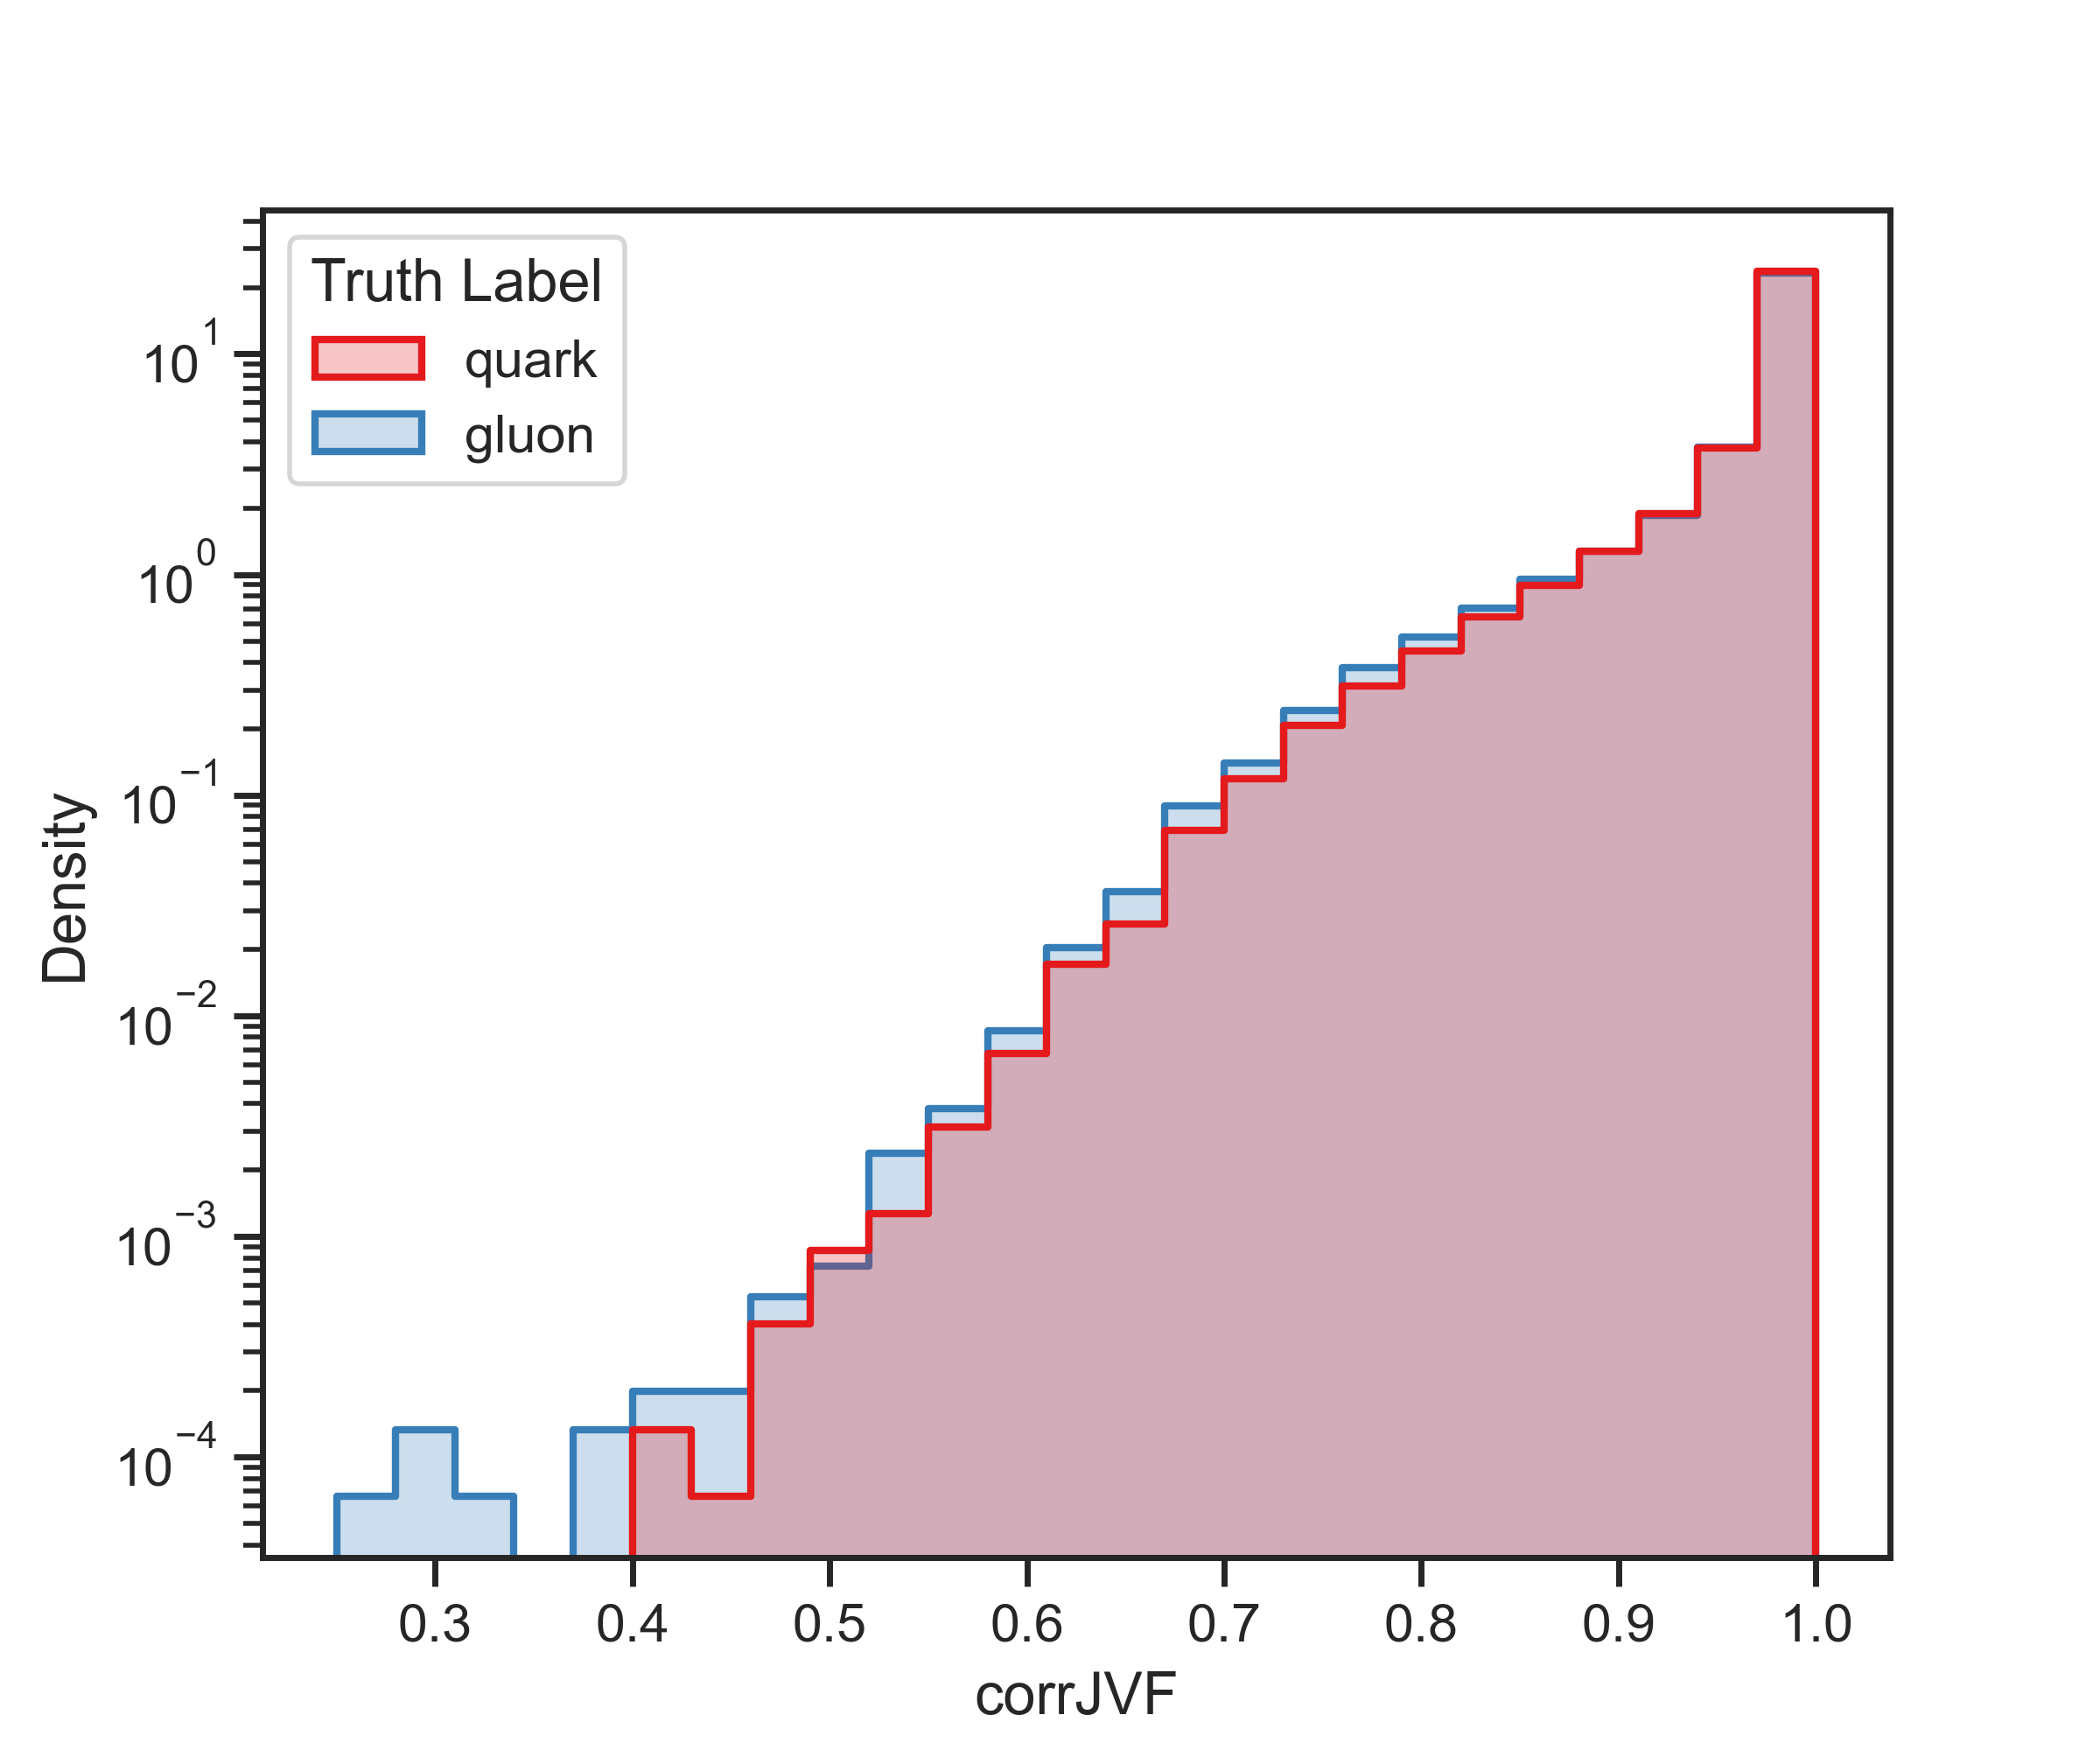
\includegraphics[width=1\textwidth]{src/plots/distributions/highlevel/jets_JVFCorr.png}
		\caption{\texttt{jets\_JVFCorr}}
		\label{fig:highlevel_9}
	\end{subfigure}
	\begin{subfigure}[t]{0.49\textwidth}
		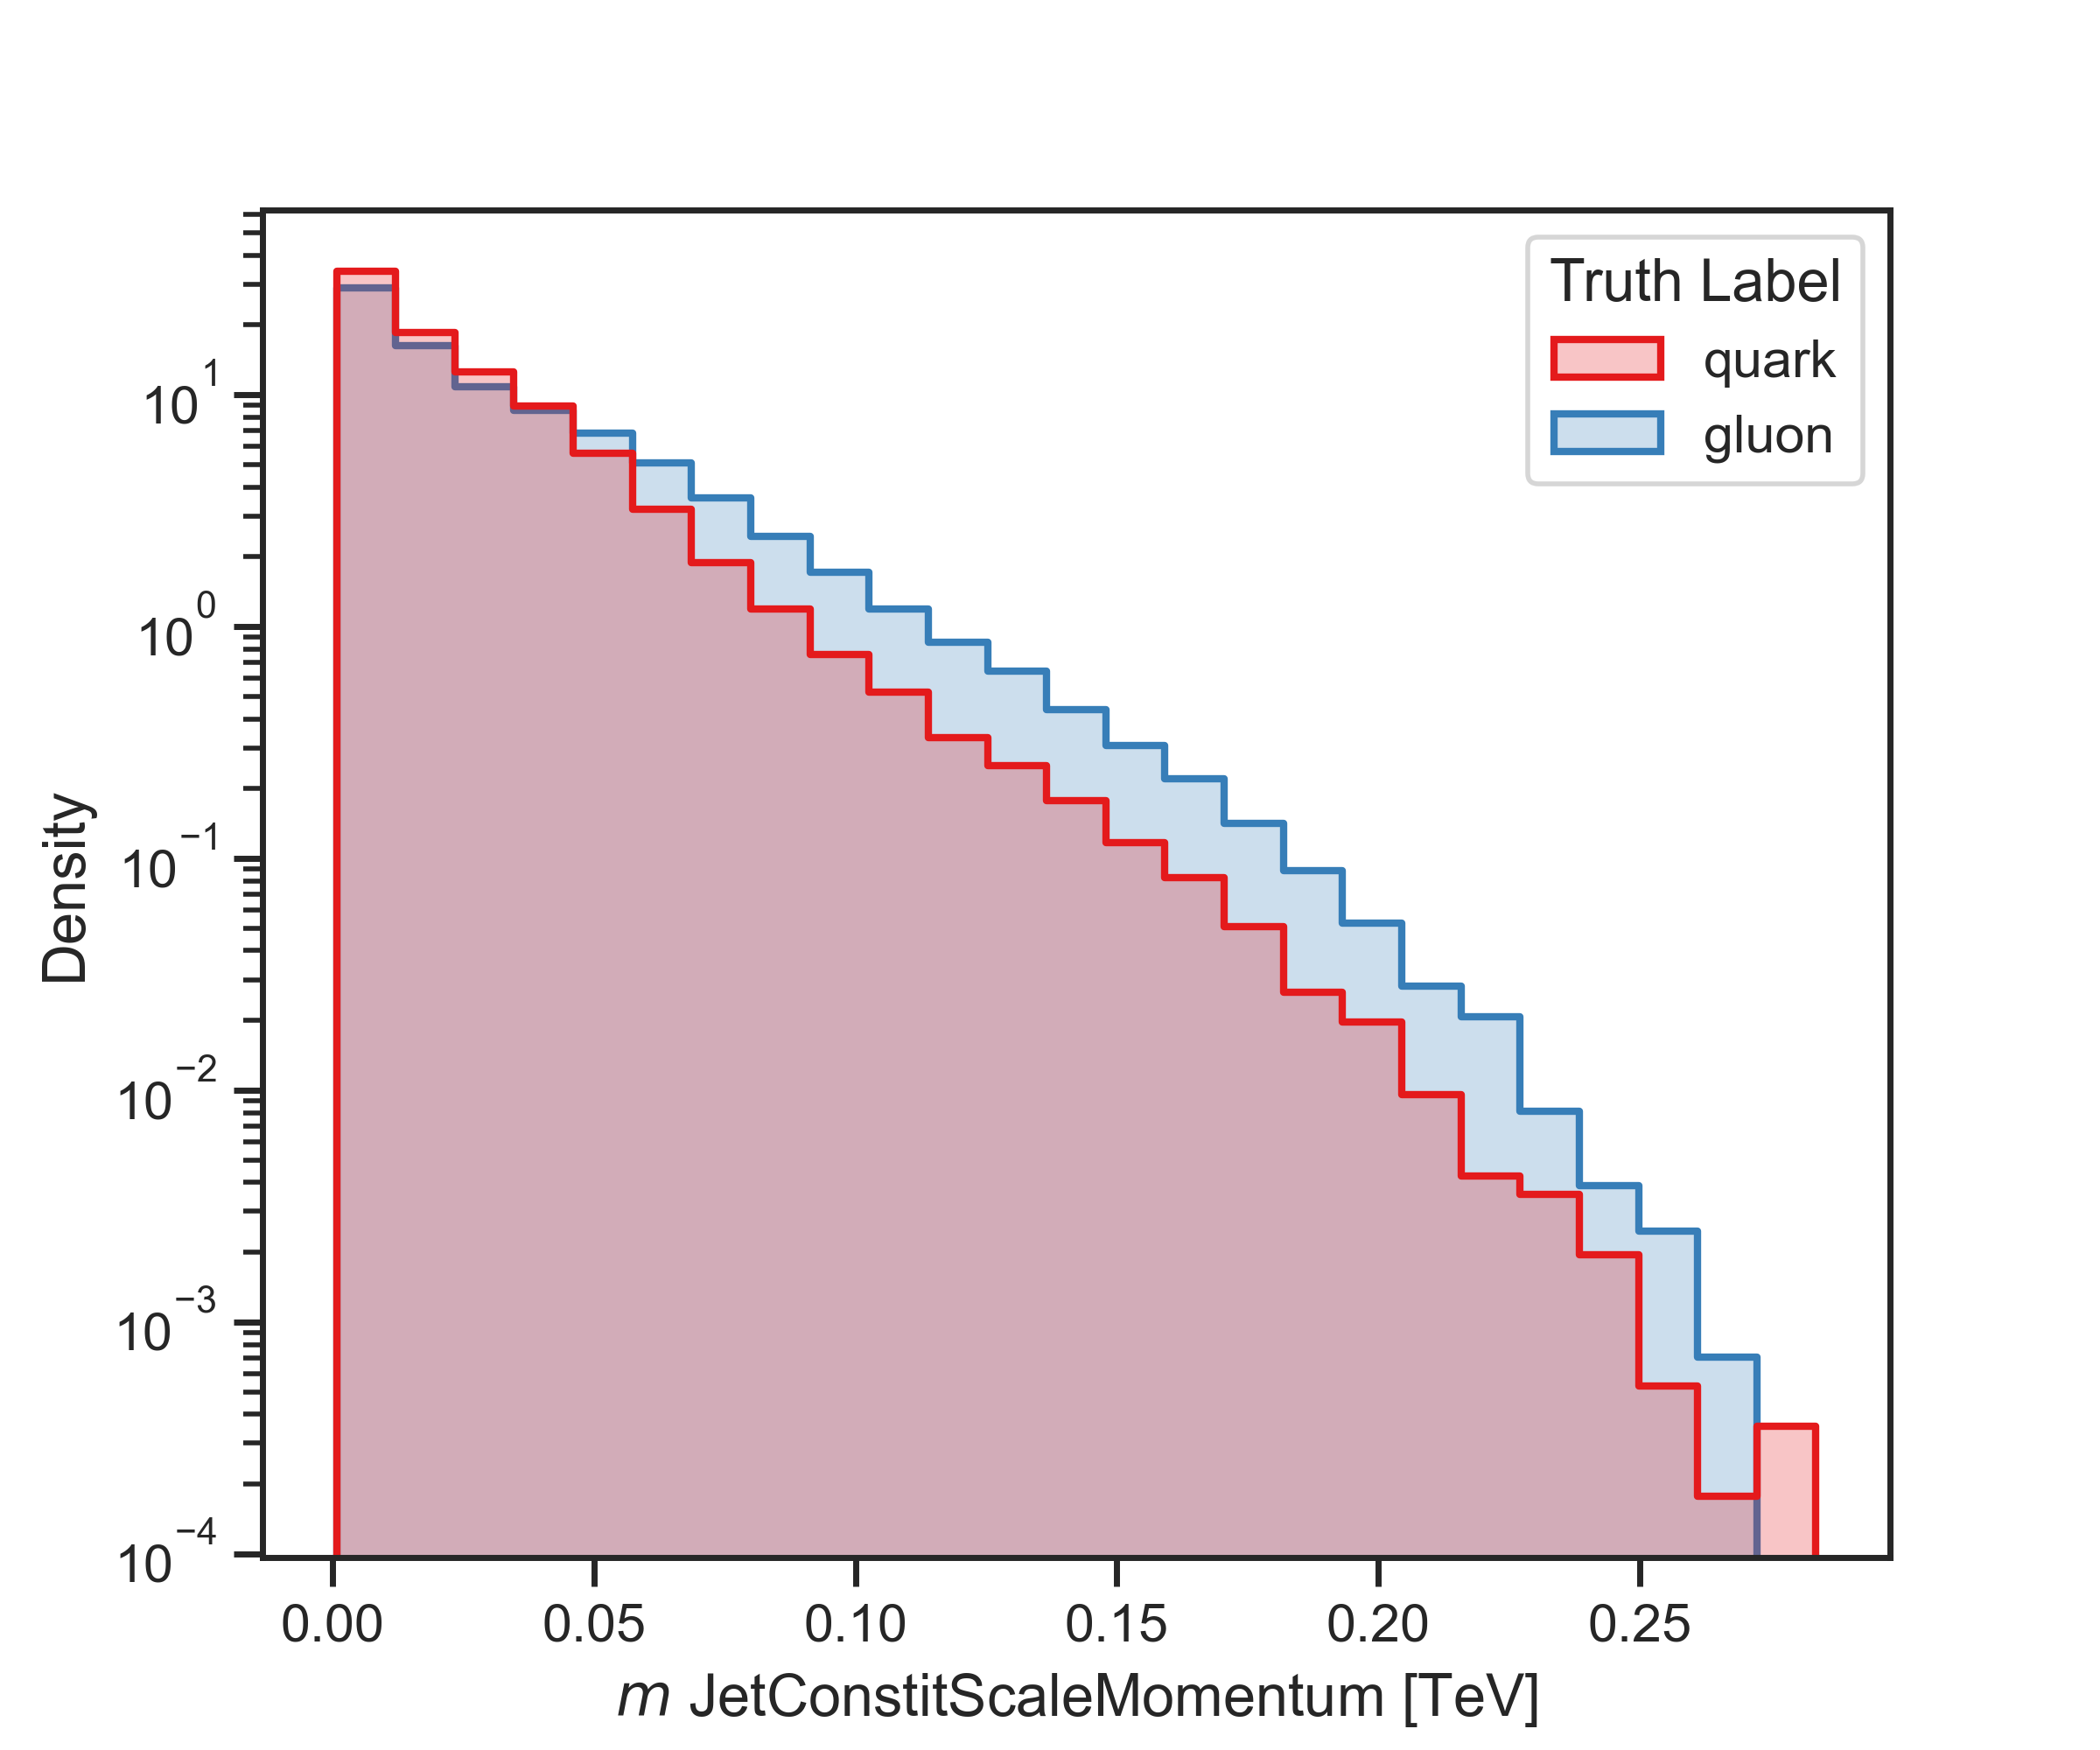
\includegraphics[width=1\textwidth]{src/plots/distributions/highlevel/jets_JetConstitScaleMomentum_m.png}
		\caption{\texttt{jets\_JetConstitScaleMomentum\_m}}
		\label{fig:highlevel_10}
	\end{subfigure}
	\begin{subfigure}[t]{0.49\textwidth}
		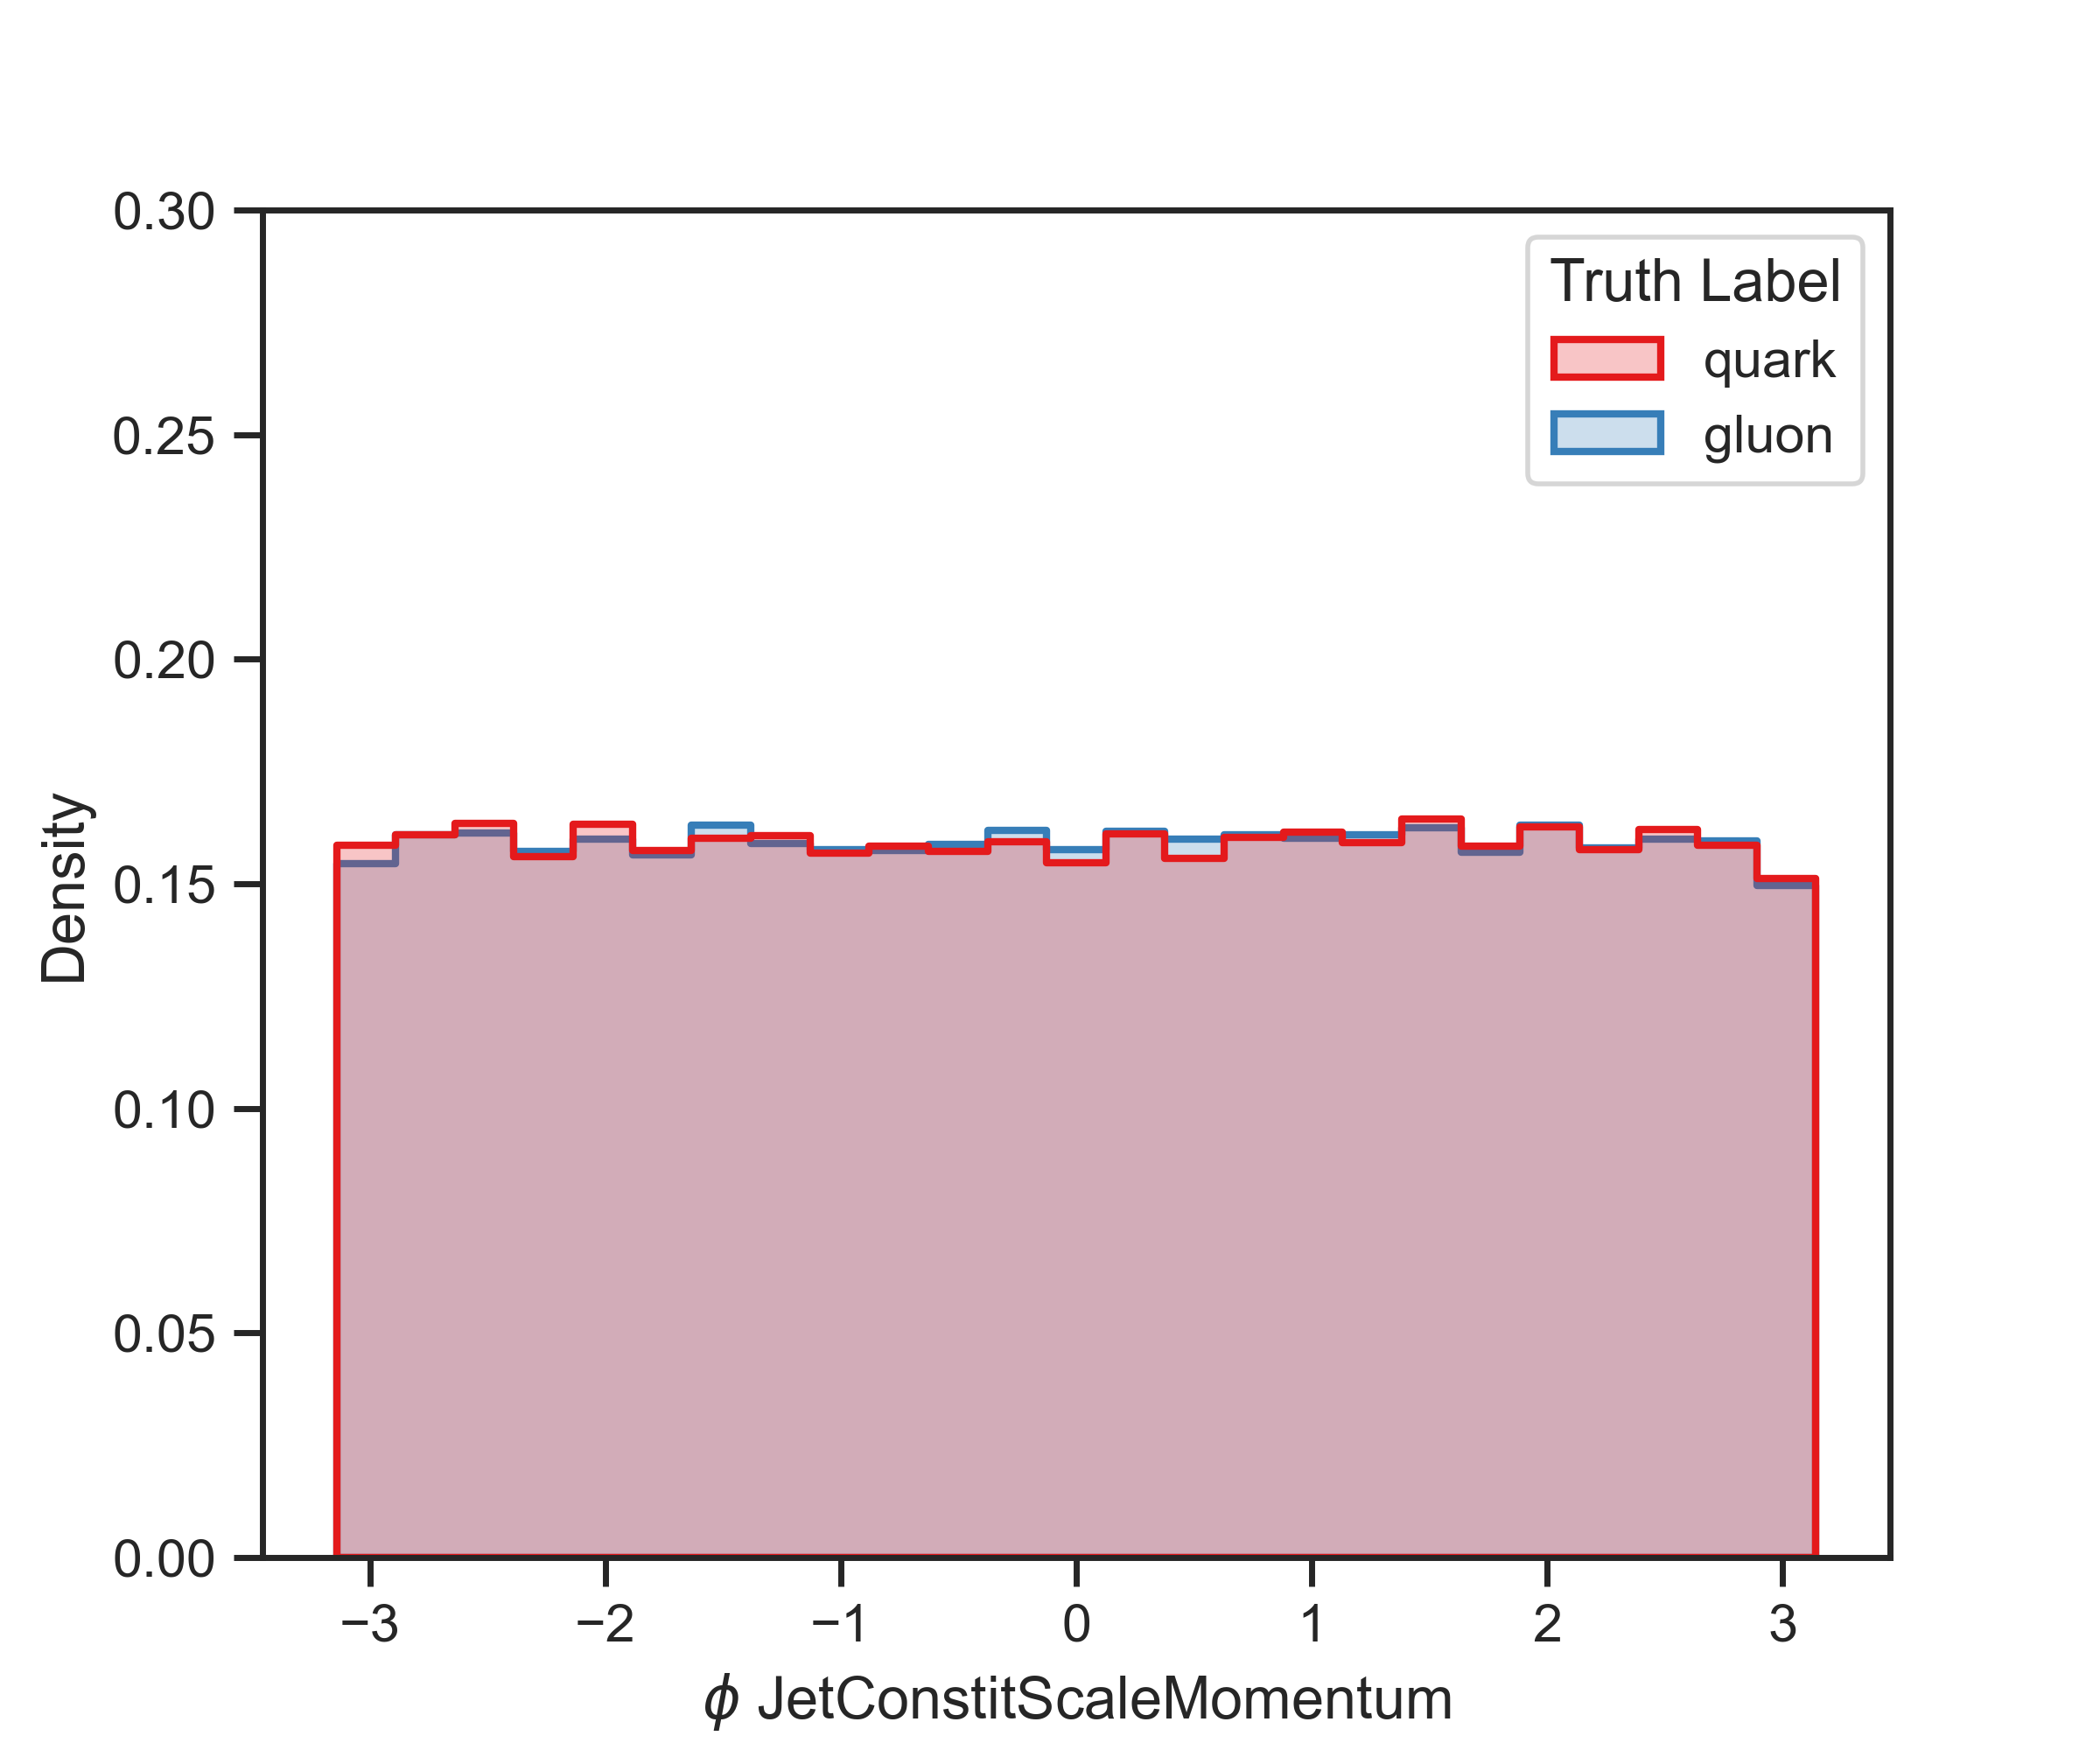
\includegraphics[width=1\textwidth]{src/plots/distributions/highlevel/jets_JetConstitScaleMomentum_phi.png}
		\caption{\texttt{jets\_JetConstitScaleMomentum\_phi}}
		\label{fig:highlevel_11}
	\end{subfigure}
\caption{High-level Jet Variables, part 2}
\label{fig:highlevel_6-11}
\end{figure}

\begin{figure}[!htb]
	\centering
	\begin{subfigure}[t]{0.49\textwidth}
		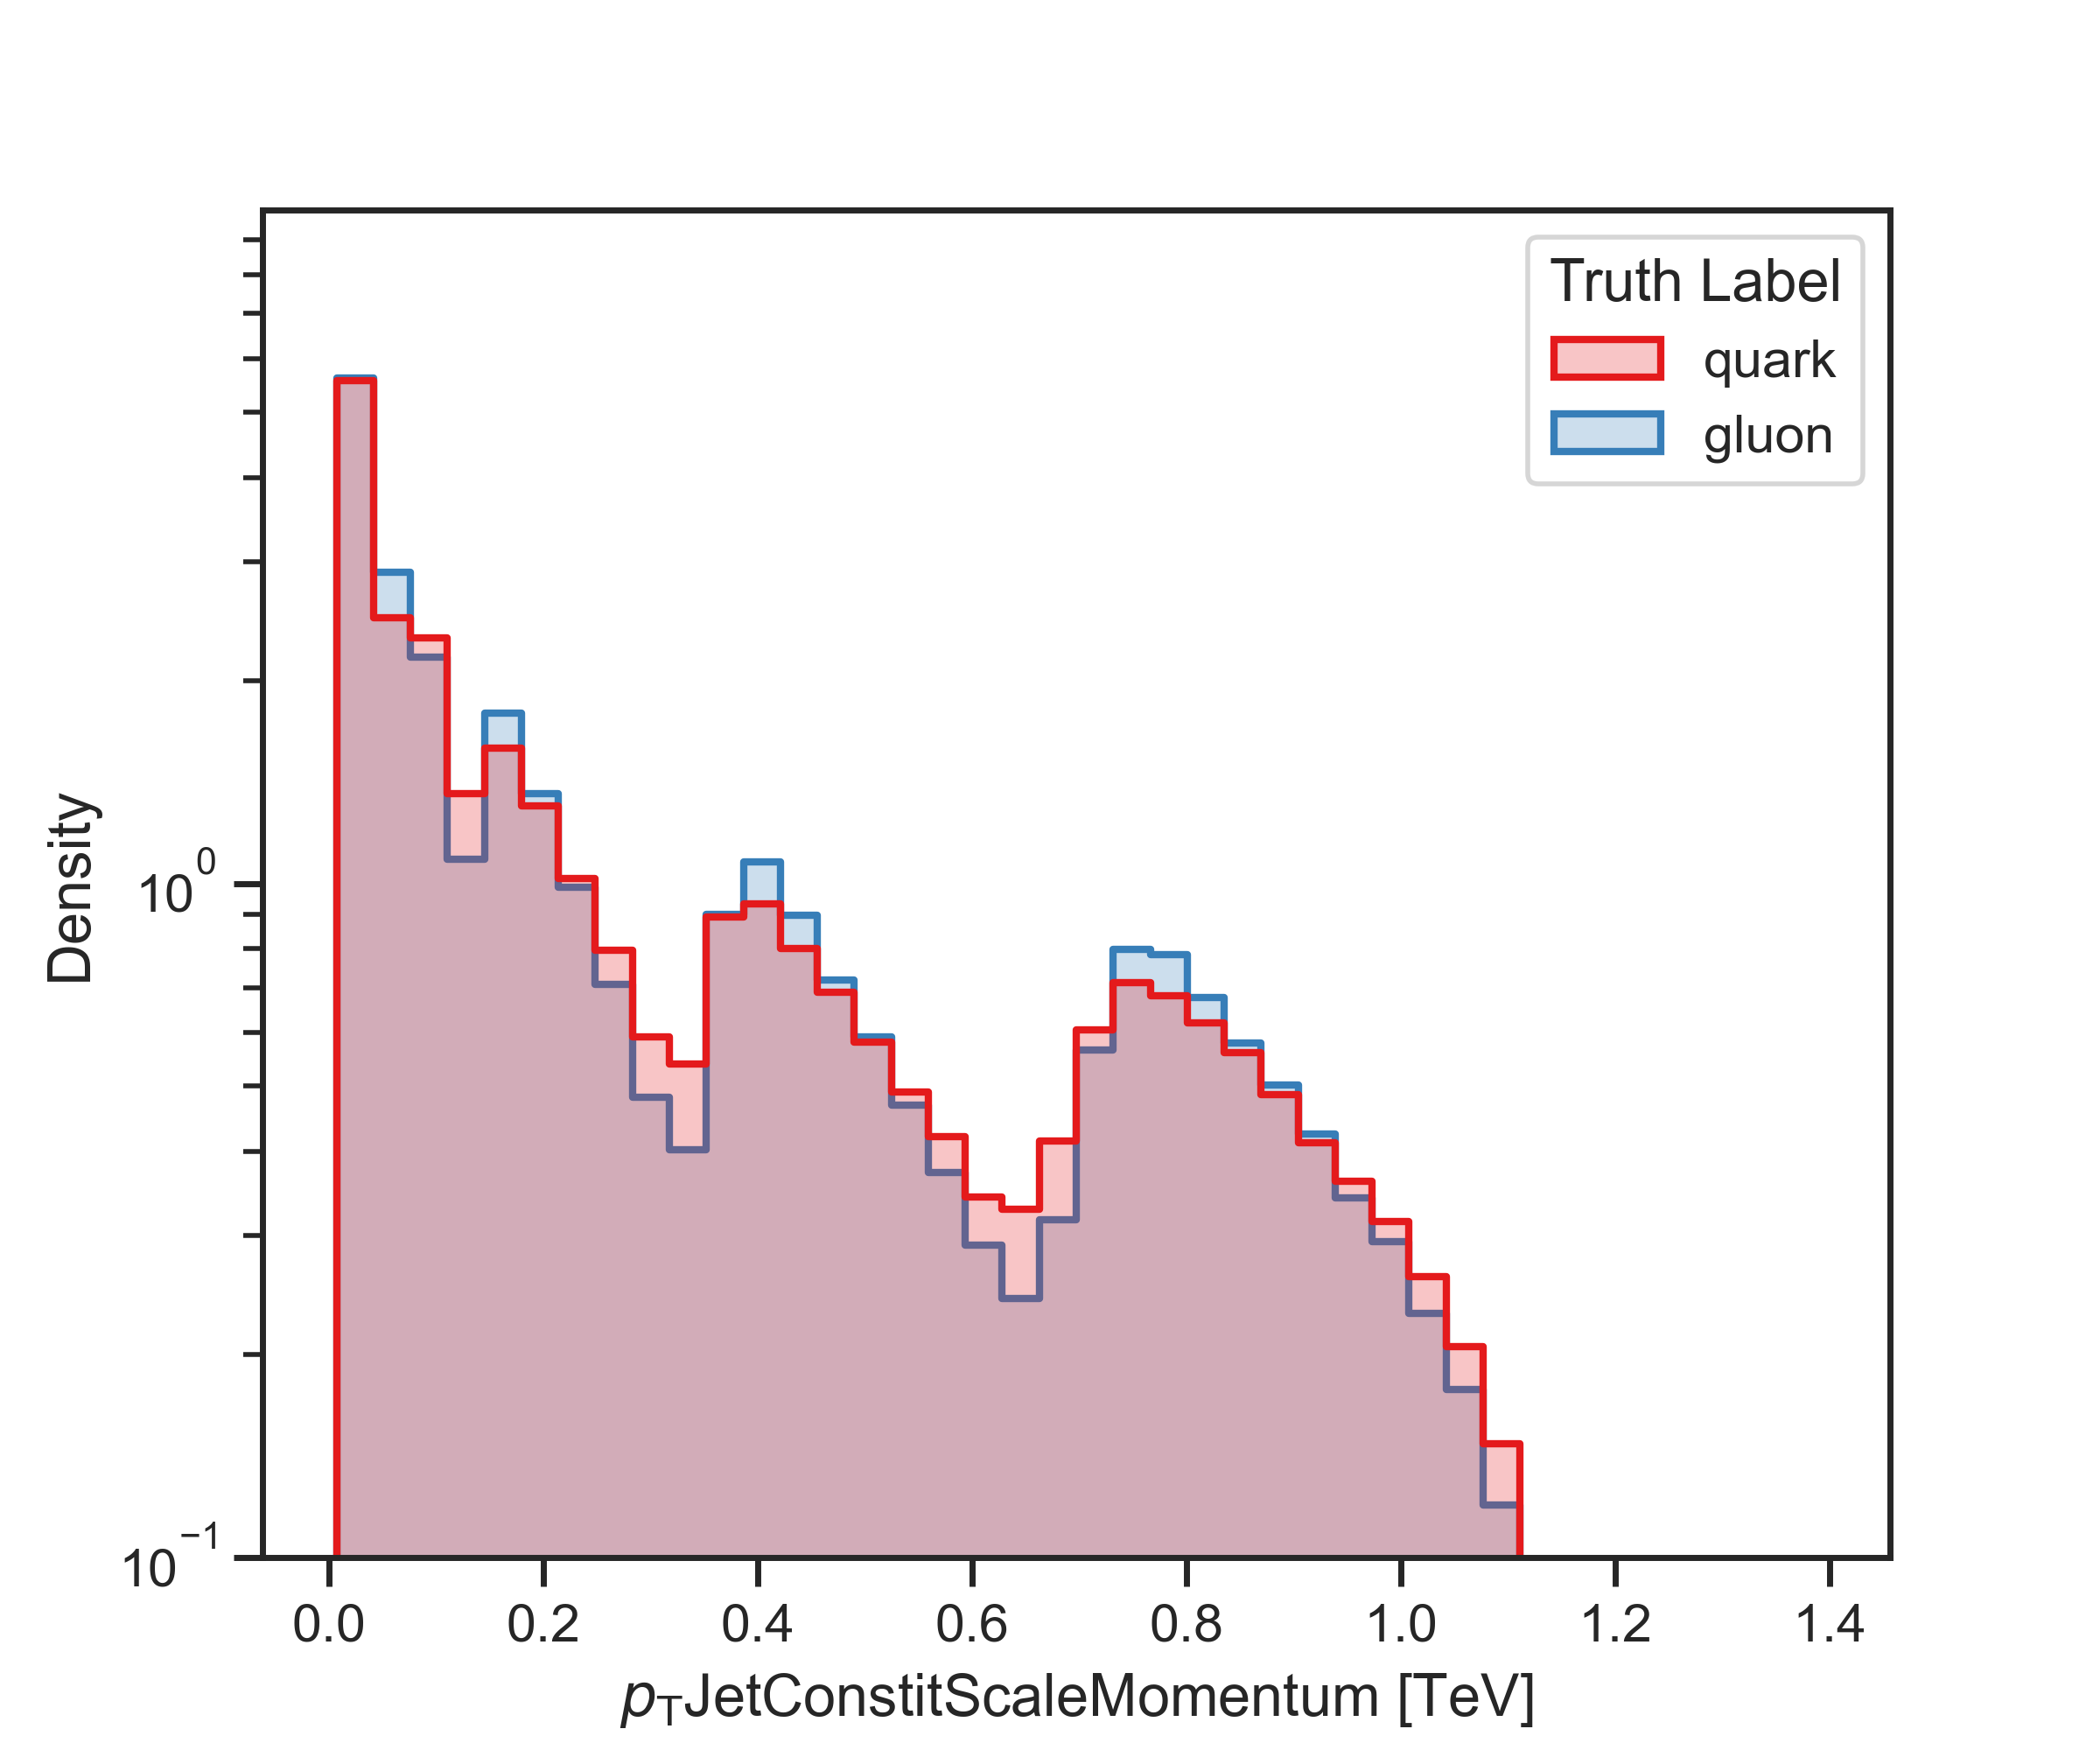
\includegraphics[width=1\textwidth]{src/plots/distributions/highlevel/jets_JetConstitScaleMomentum_pt.png}
		\caption{\texttt{jets\_JetConstitScaleMomentum\_pt}}
		\label{fig:highlevel_12}
	\end{subfigure}
	\begin{subfigure}[t]{0.49\textwidth}
		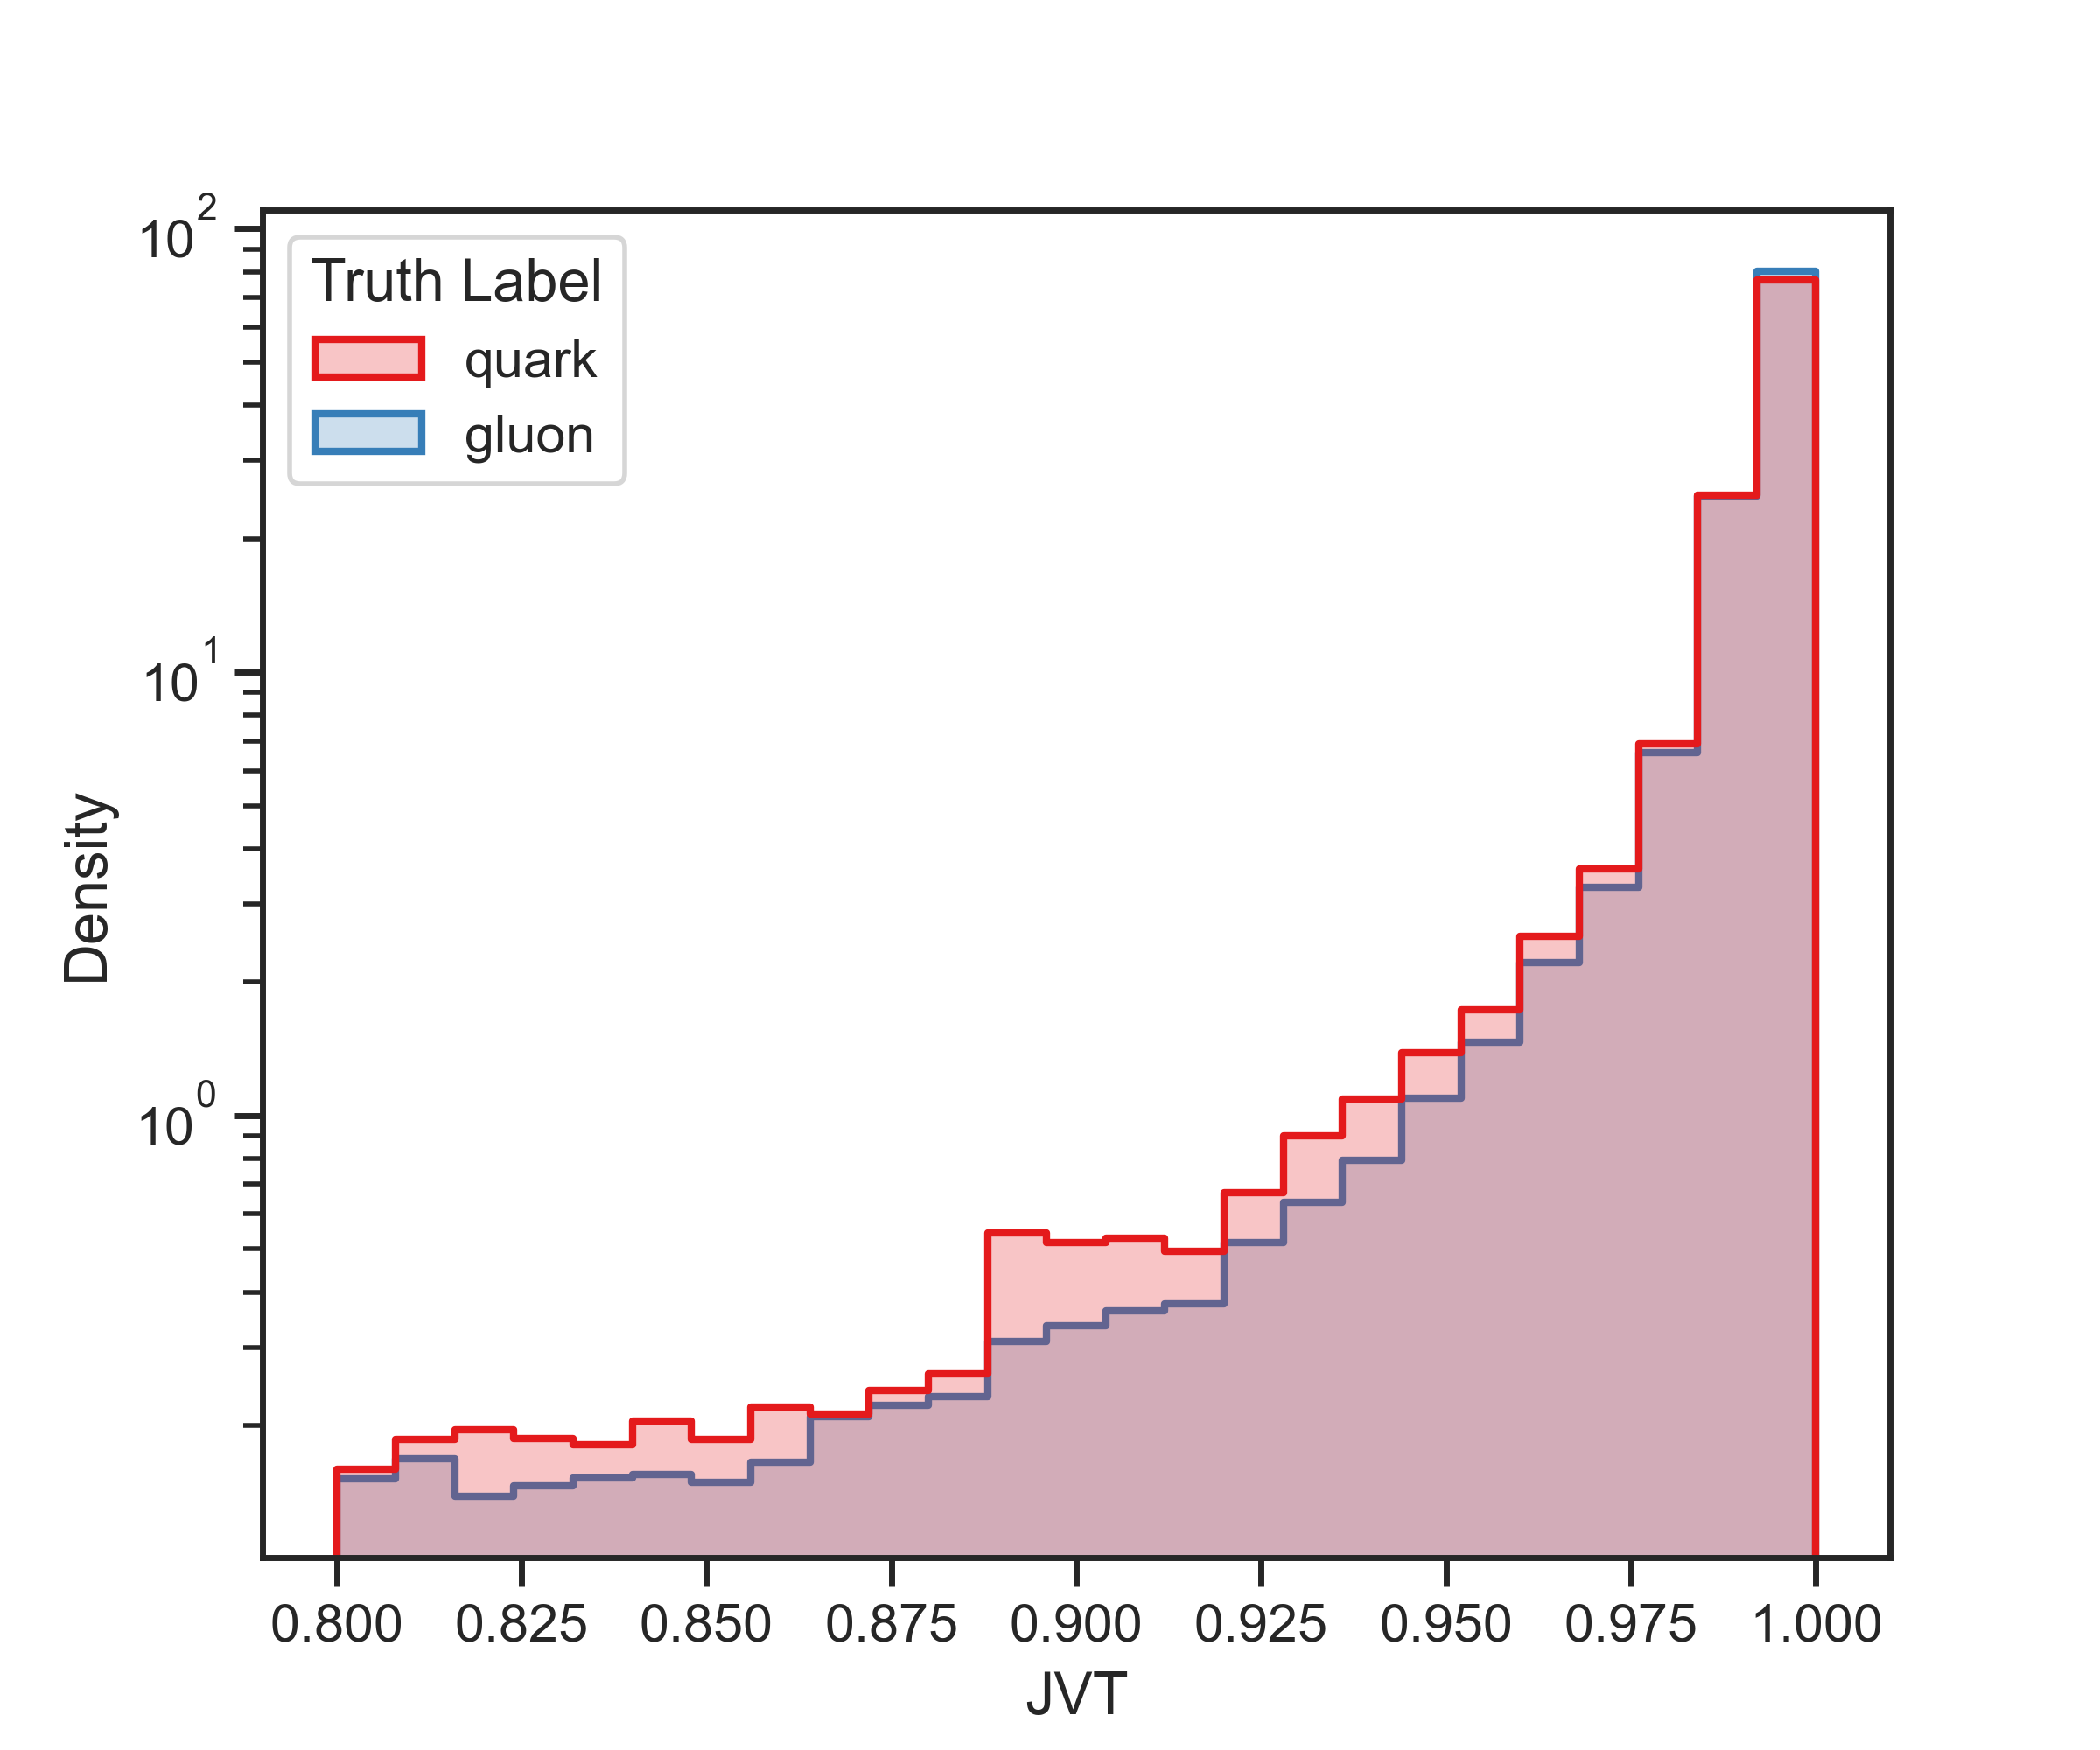
\includegraphics[width=1\textwidth]{src/plots/distributions/highlevel/jets_Jvt.png}
		\caption{\texttt{jets\_Jvt}}
		\label{fig:highlevel_13}
	\end{subfigure}
	\begin{subfigure}[t]{0.49\textwidth}
		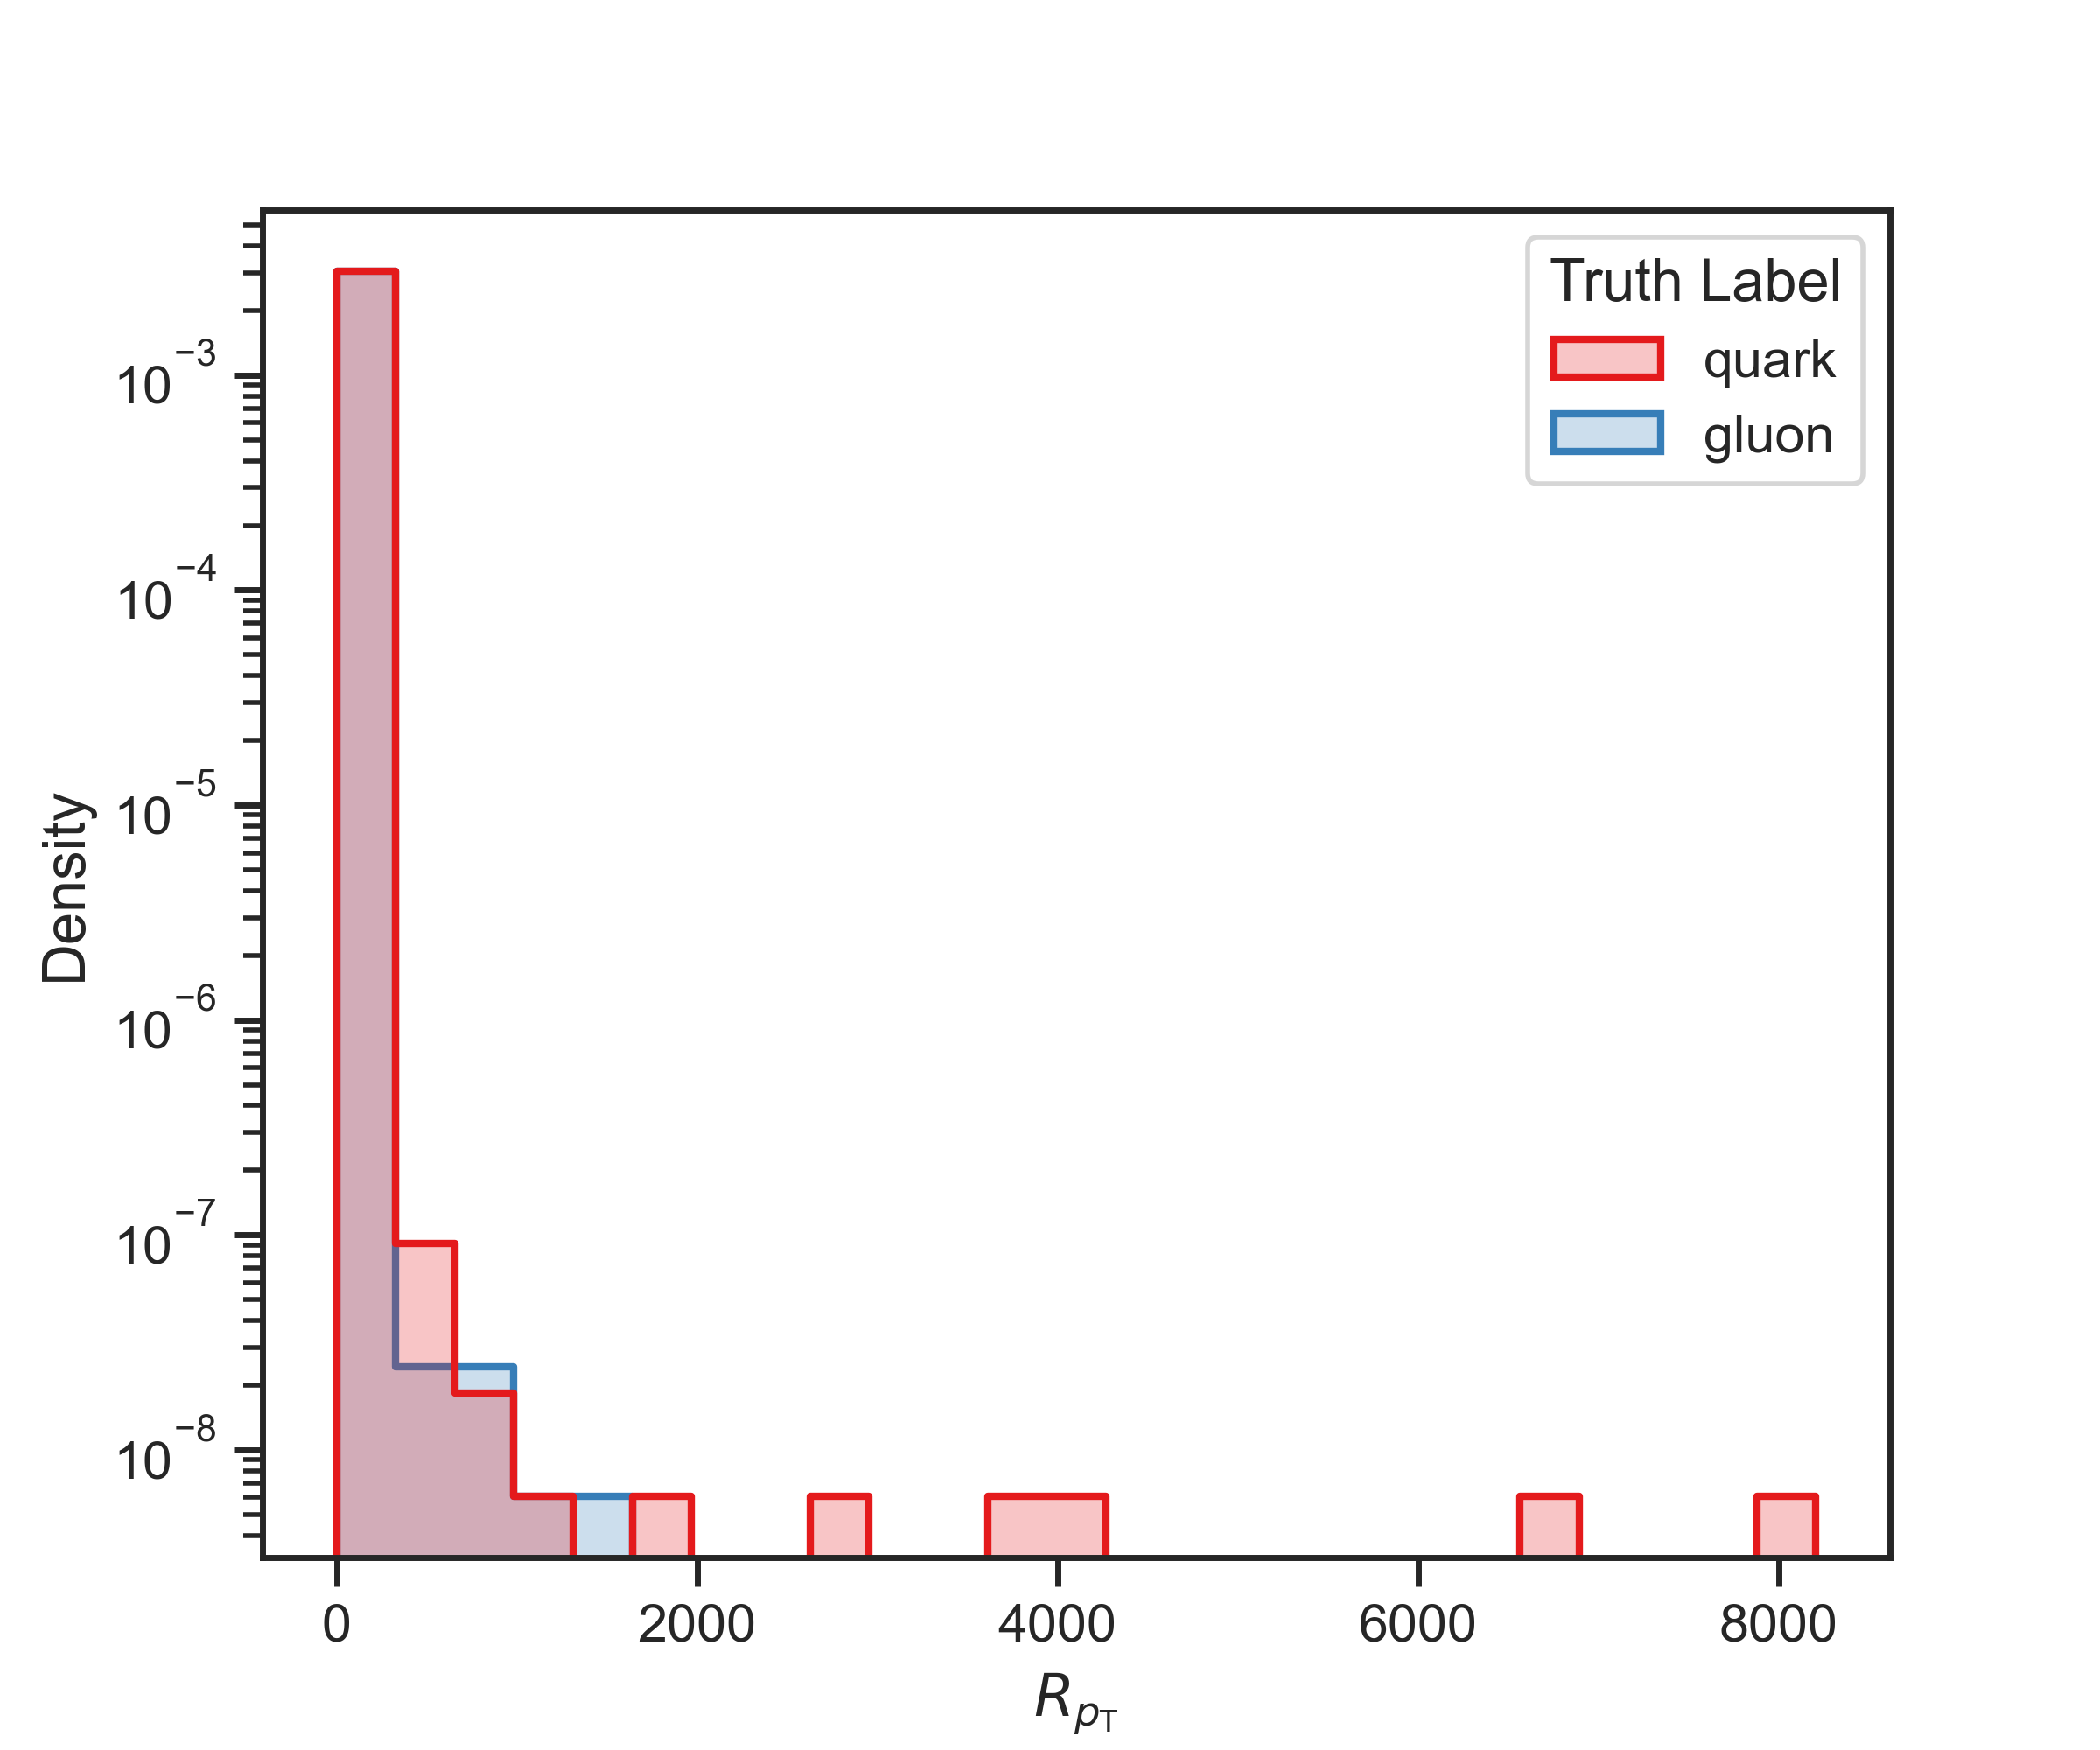
\includegraphics[width=1\textwidth]{src/plots/distributions/highlevel/jets_JvtRpt.png}
		\caption{\texttt{jets\_JvtRpt}}
		\label{fig:highlevel_14}
	\end{subfigure}
	\begin{subfigure}[t]{0.49\textwidth}
		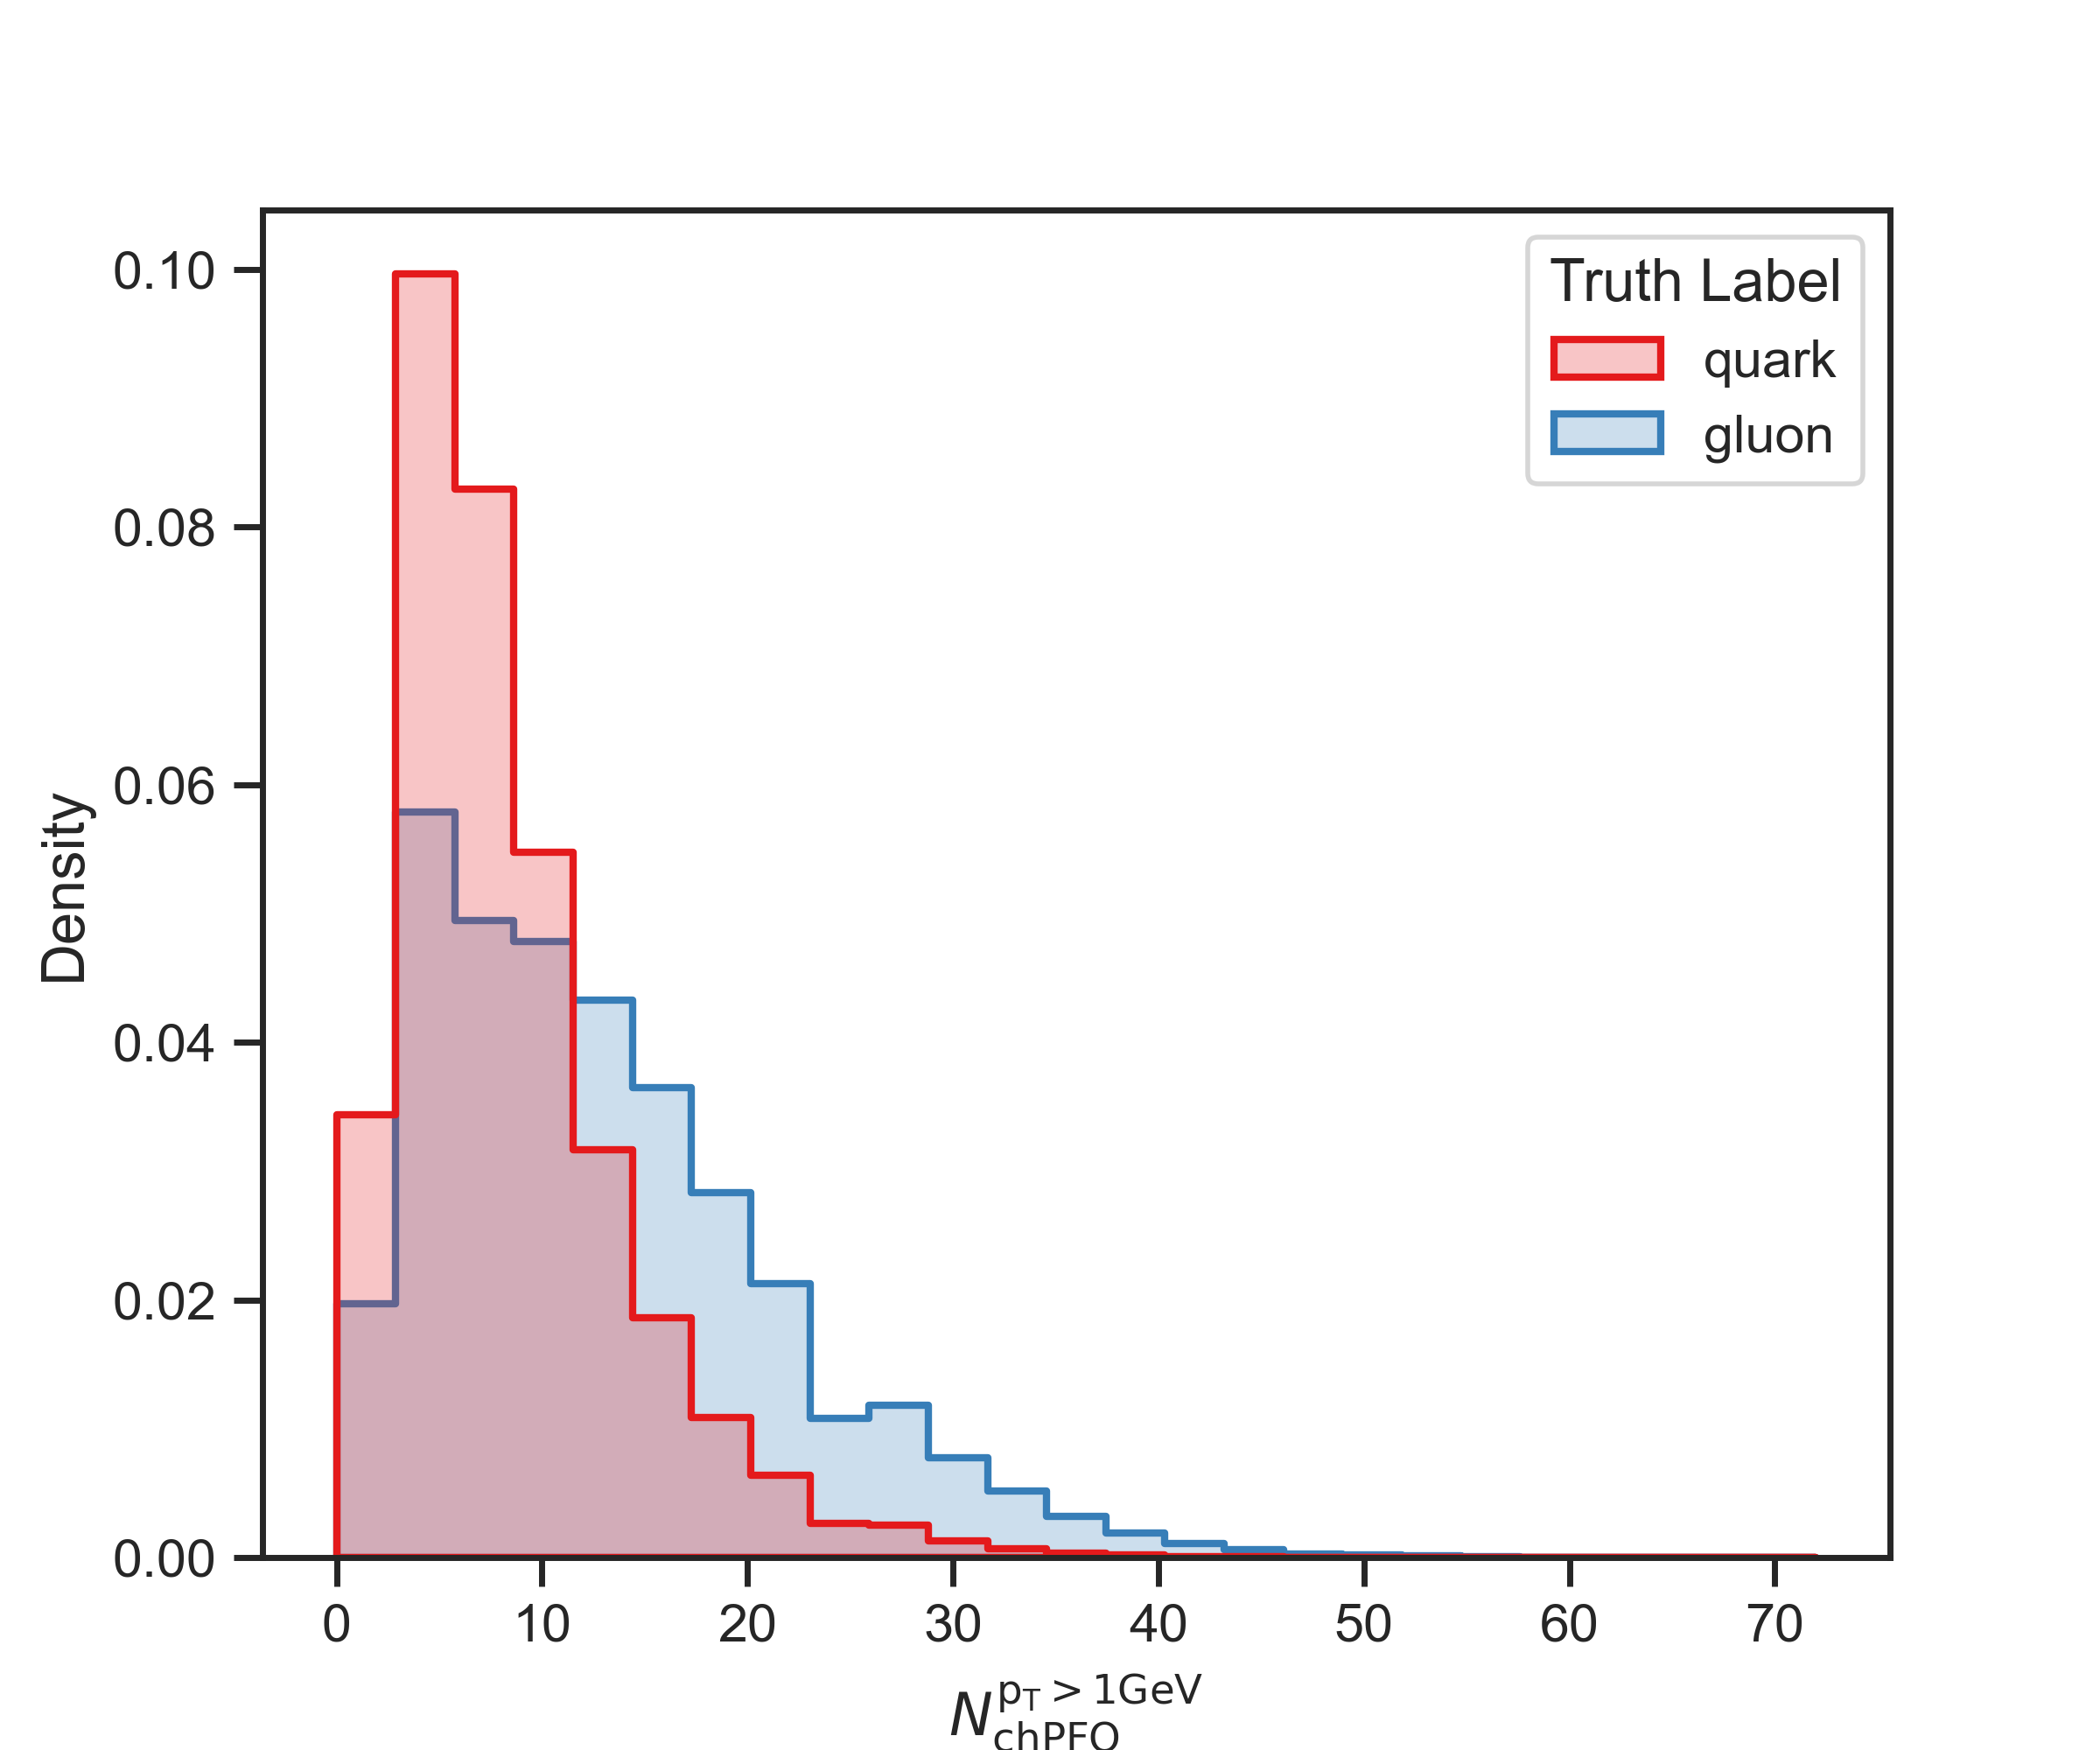
\includegraphics[width=1\textwidth]{src/plots/distributions/highlevel/jets_NumChargedPFOPt1000[0].png}
		\caption{\texttt{jets\_NumChargedPFOPt1000[0]}}
		\label{fig:highlevel_15}
	\end{subfigure}
	\begin{subfigure}[t]{0.49\textwidth}
		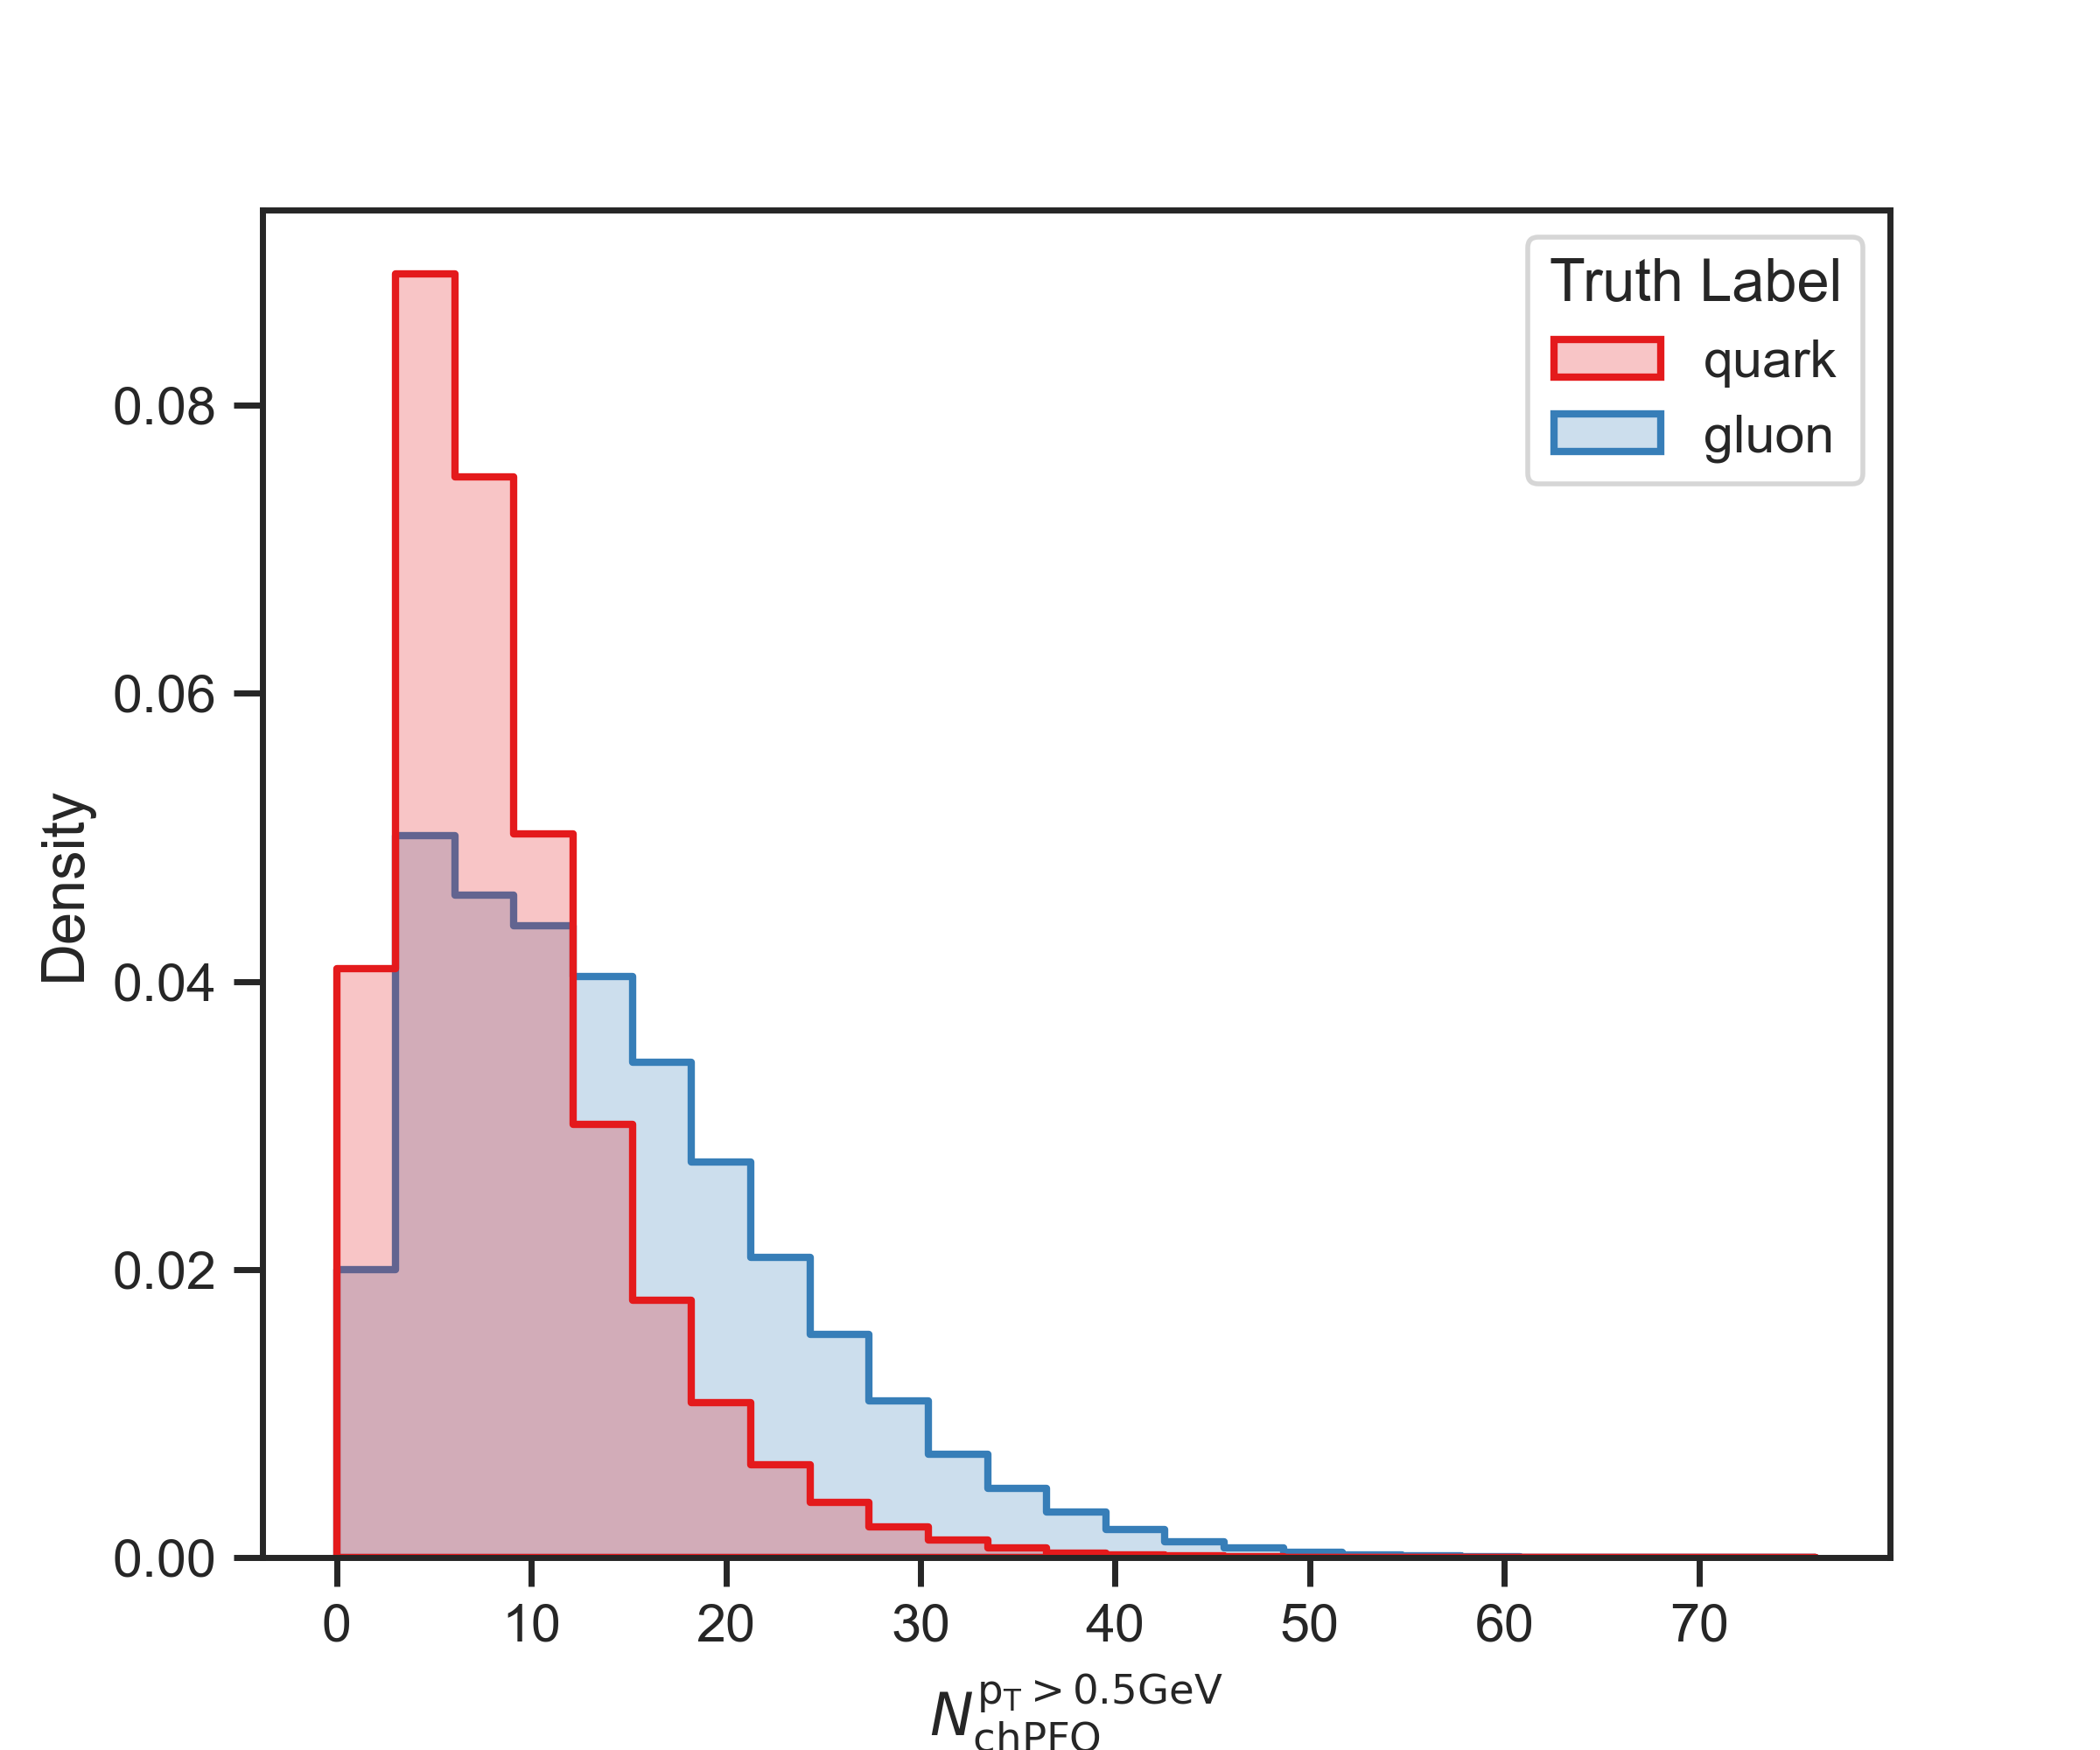
\includegraphics[width=1\textwidth]{src/plots/distributions/highlevel/jets_NumChargedPFOPt500[0].png}
		\caption{\texttt{jets\_NumChargedPFOPt500[0]}}
		\label{fig:highlevel_16}
	\end{subfigure}
	\begin{subfigure}[t]{0.49\textwidth}
		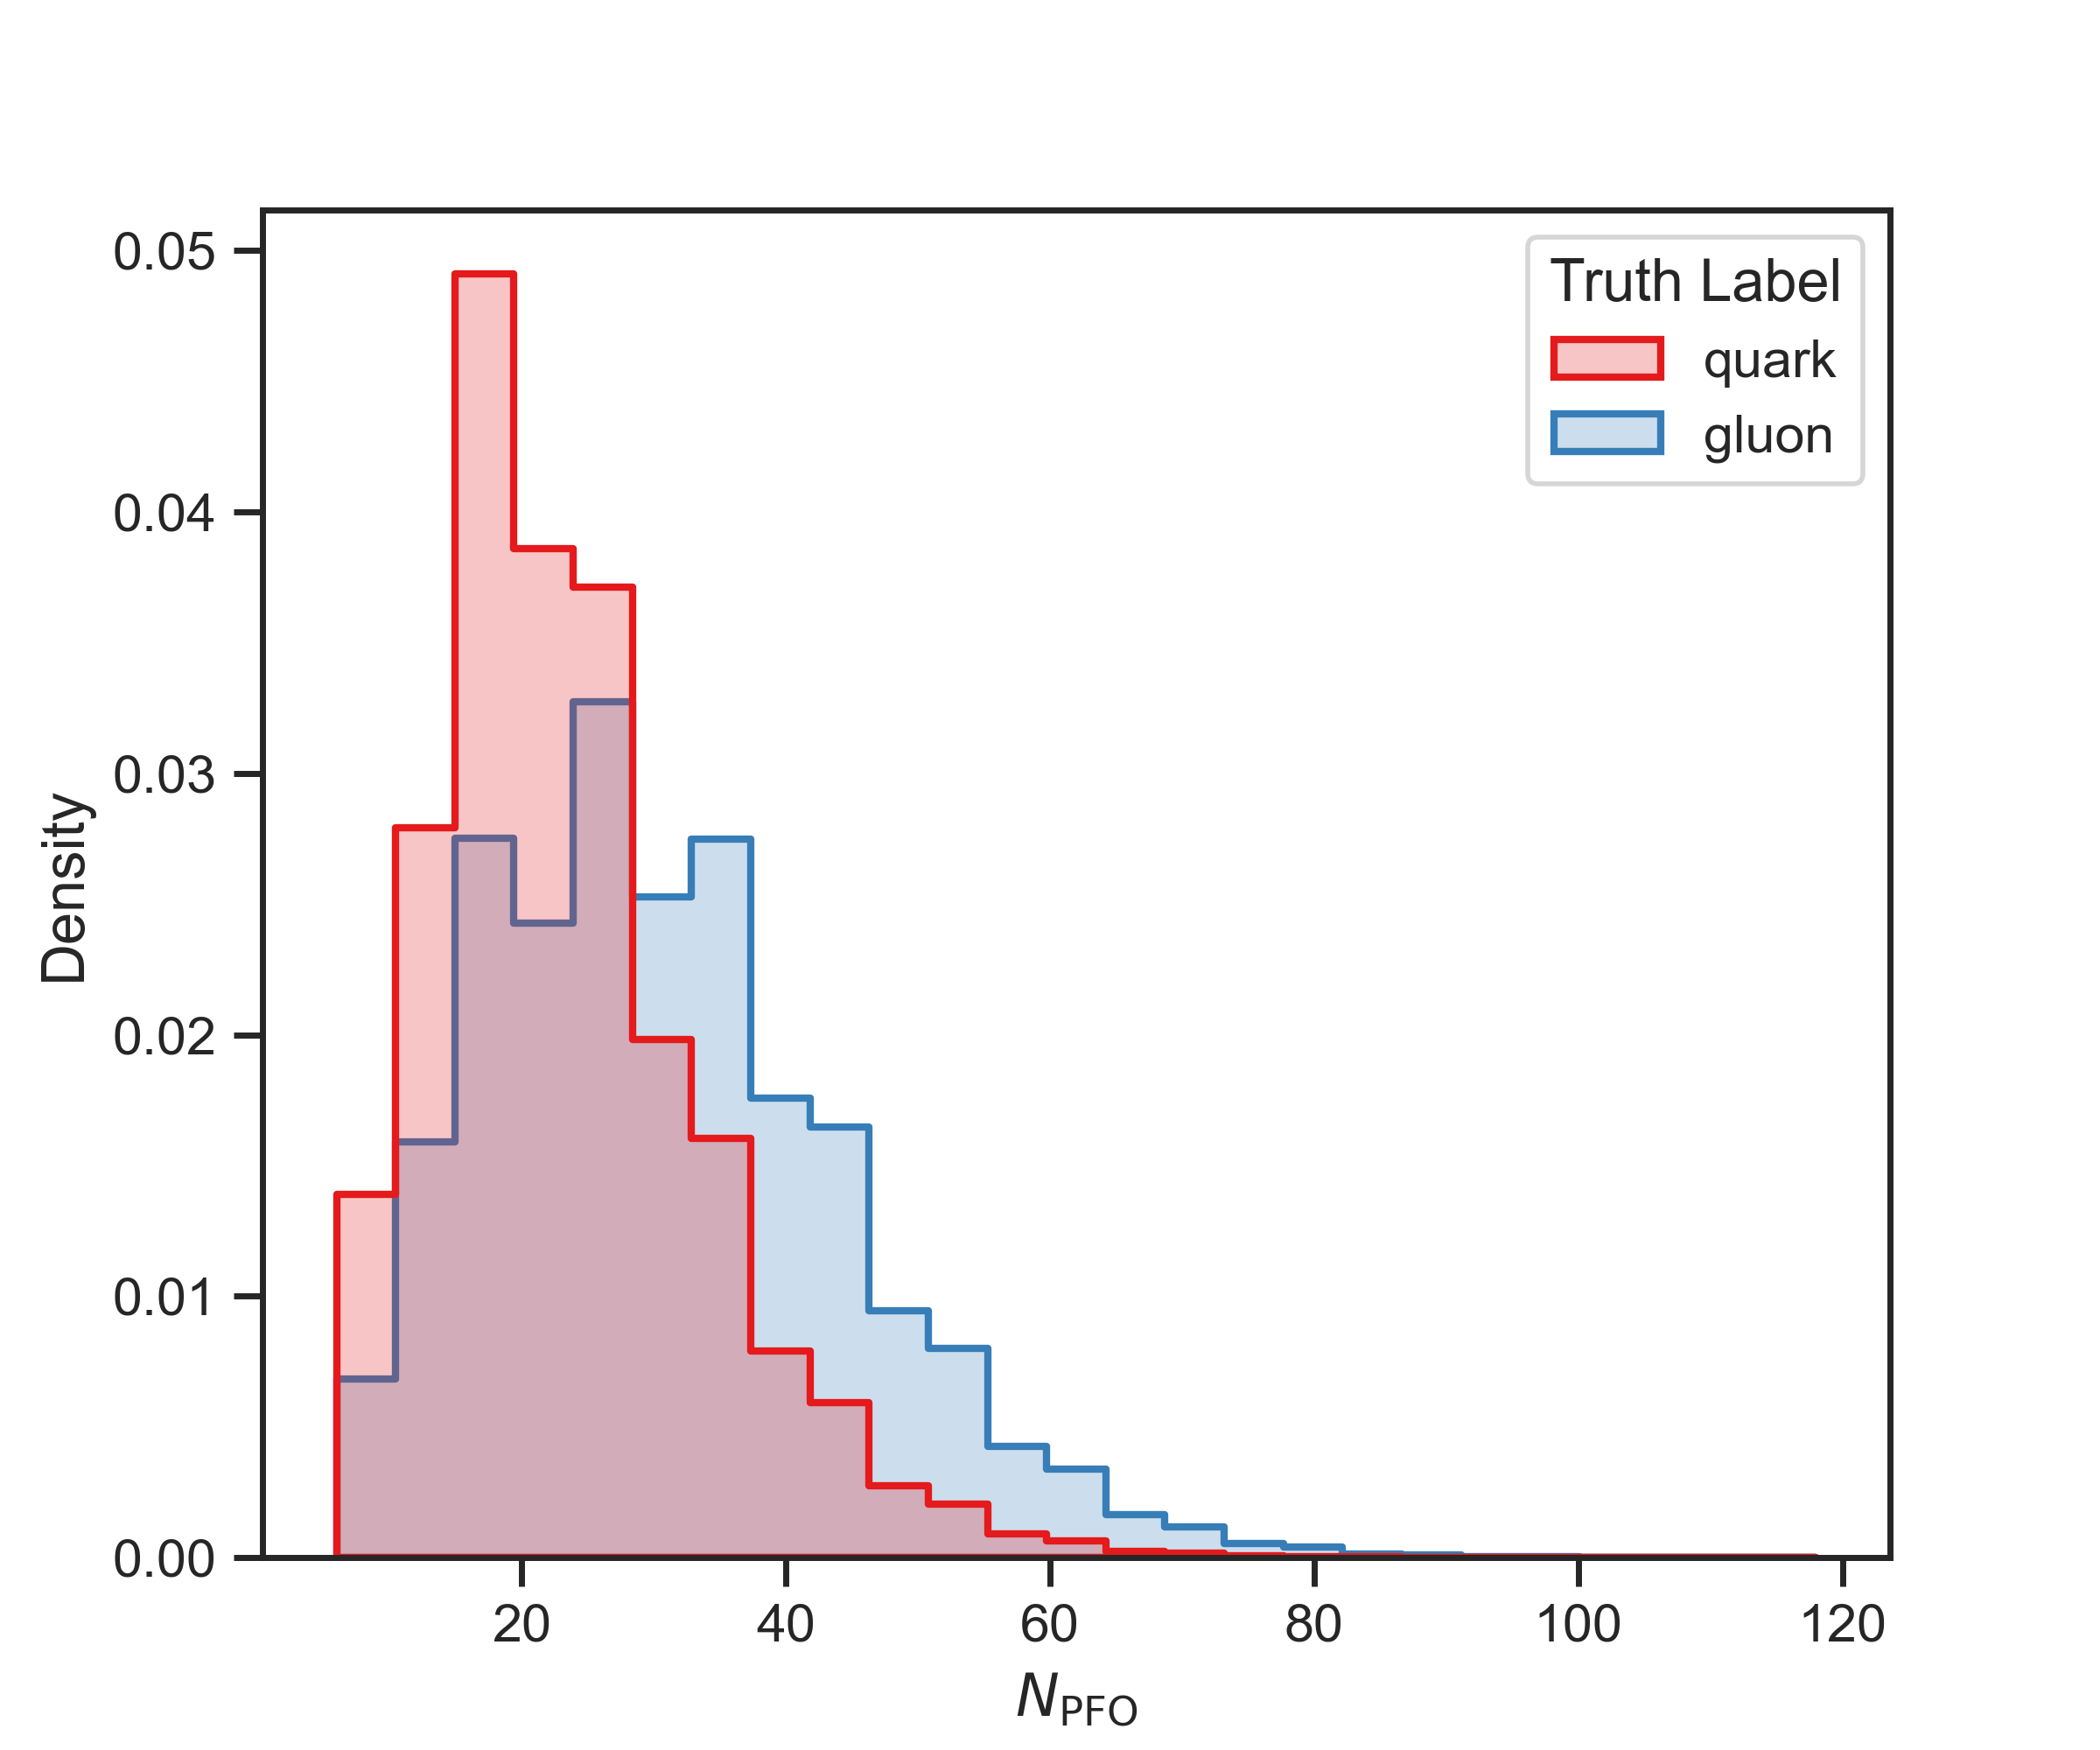
\includegraphics[width=1\textwidth]{src/plots/distributions/highlevel/jets_PFO_n.png}
		\caption{\texttt{jets\_PFO\_n}}
		\label{fig:highlevel_17}
	\end{subfigure}
\caption{High-level Jet Variables, part 3}
\label{fig:highlevel_12-17}
\end{figure}

\begin{figure}[!htb]
	\centering
	\begin{subfigure}[t]{0.49\textwidth}
		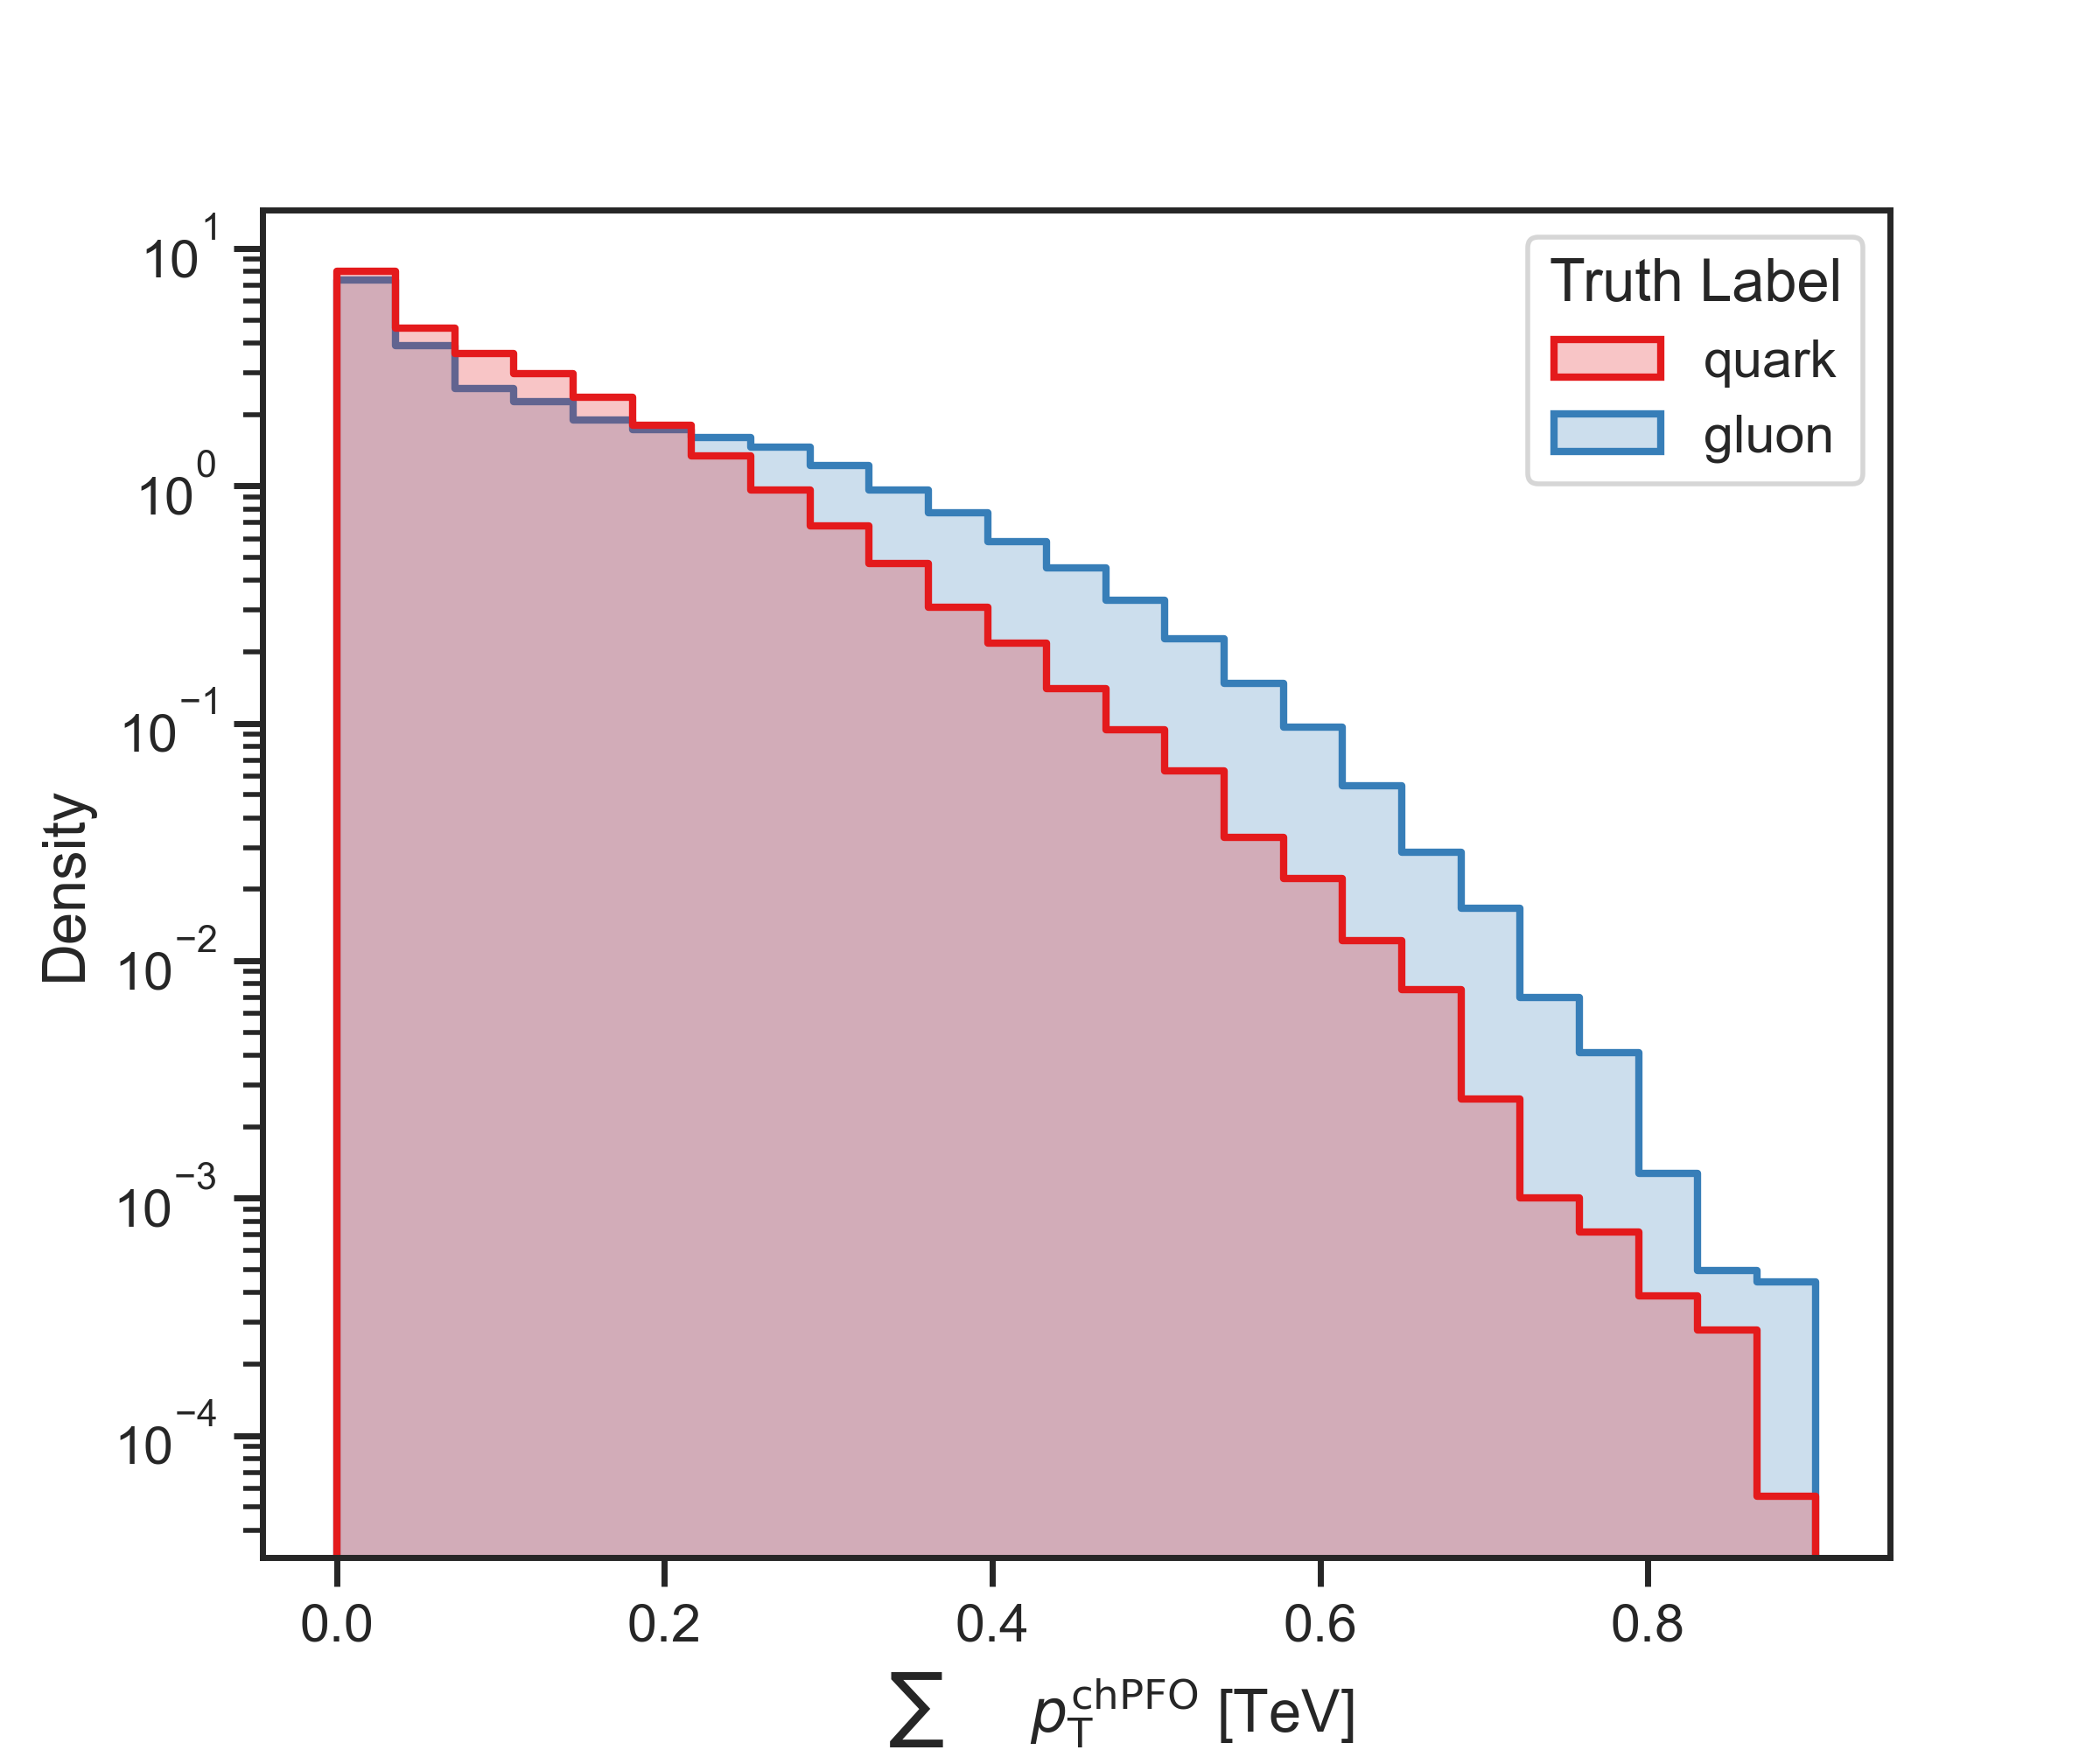
\includegraphics[width=1\textwidth]{src/plots/distributions/highlevel/jets_SumPtChargedPFOPt500[0].png}
		\caption{\texttt{jets\_SumPtChargedPFOPt500[0]}}
		\label{fig:highlevel_18}
	\end{subfigure}
	\begin{subfigure}[t]{0.49\textwidth}
		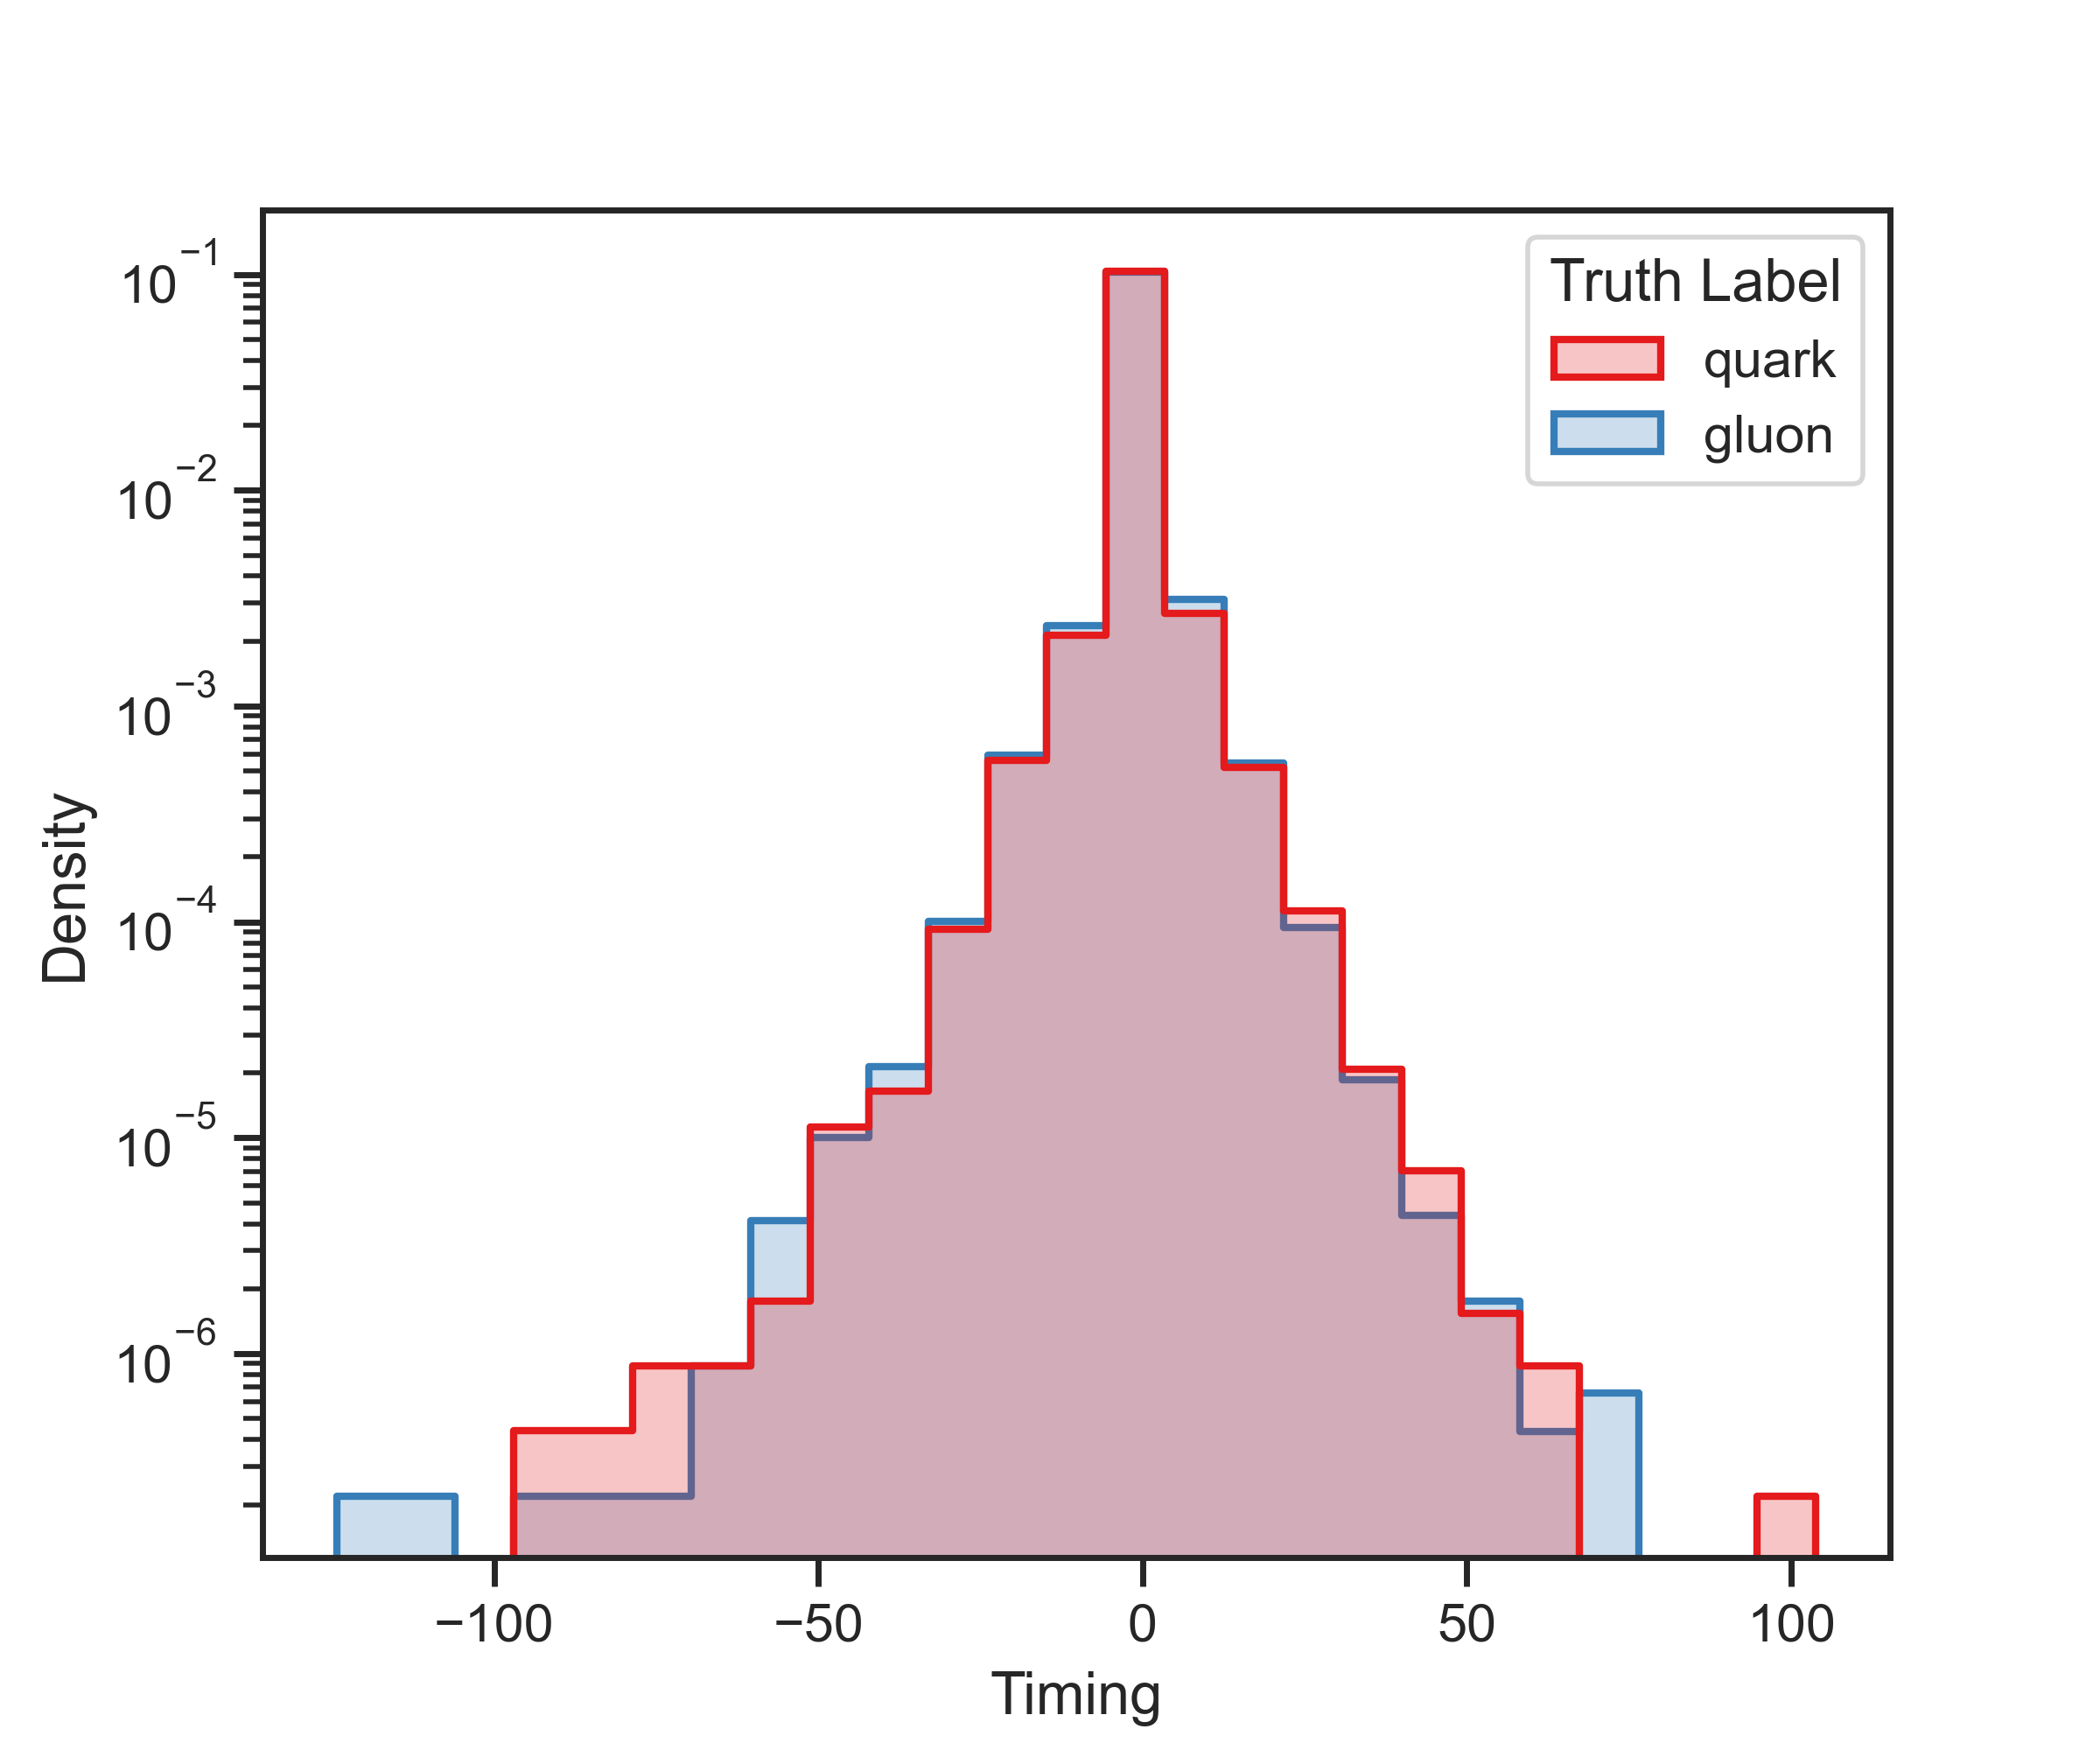
\includegraphics[width=1\textwidth]{src/plots/distributions/highlevel/jets_Timing.png}
		\caption{\texttt{jets\_Timing}}
		\label{fig:highlevel_19}
	\end{subfigure}
	\begin{subfigure}[t]{0.49\textwidth}
		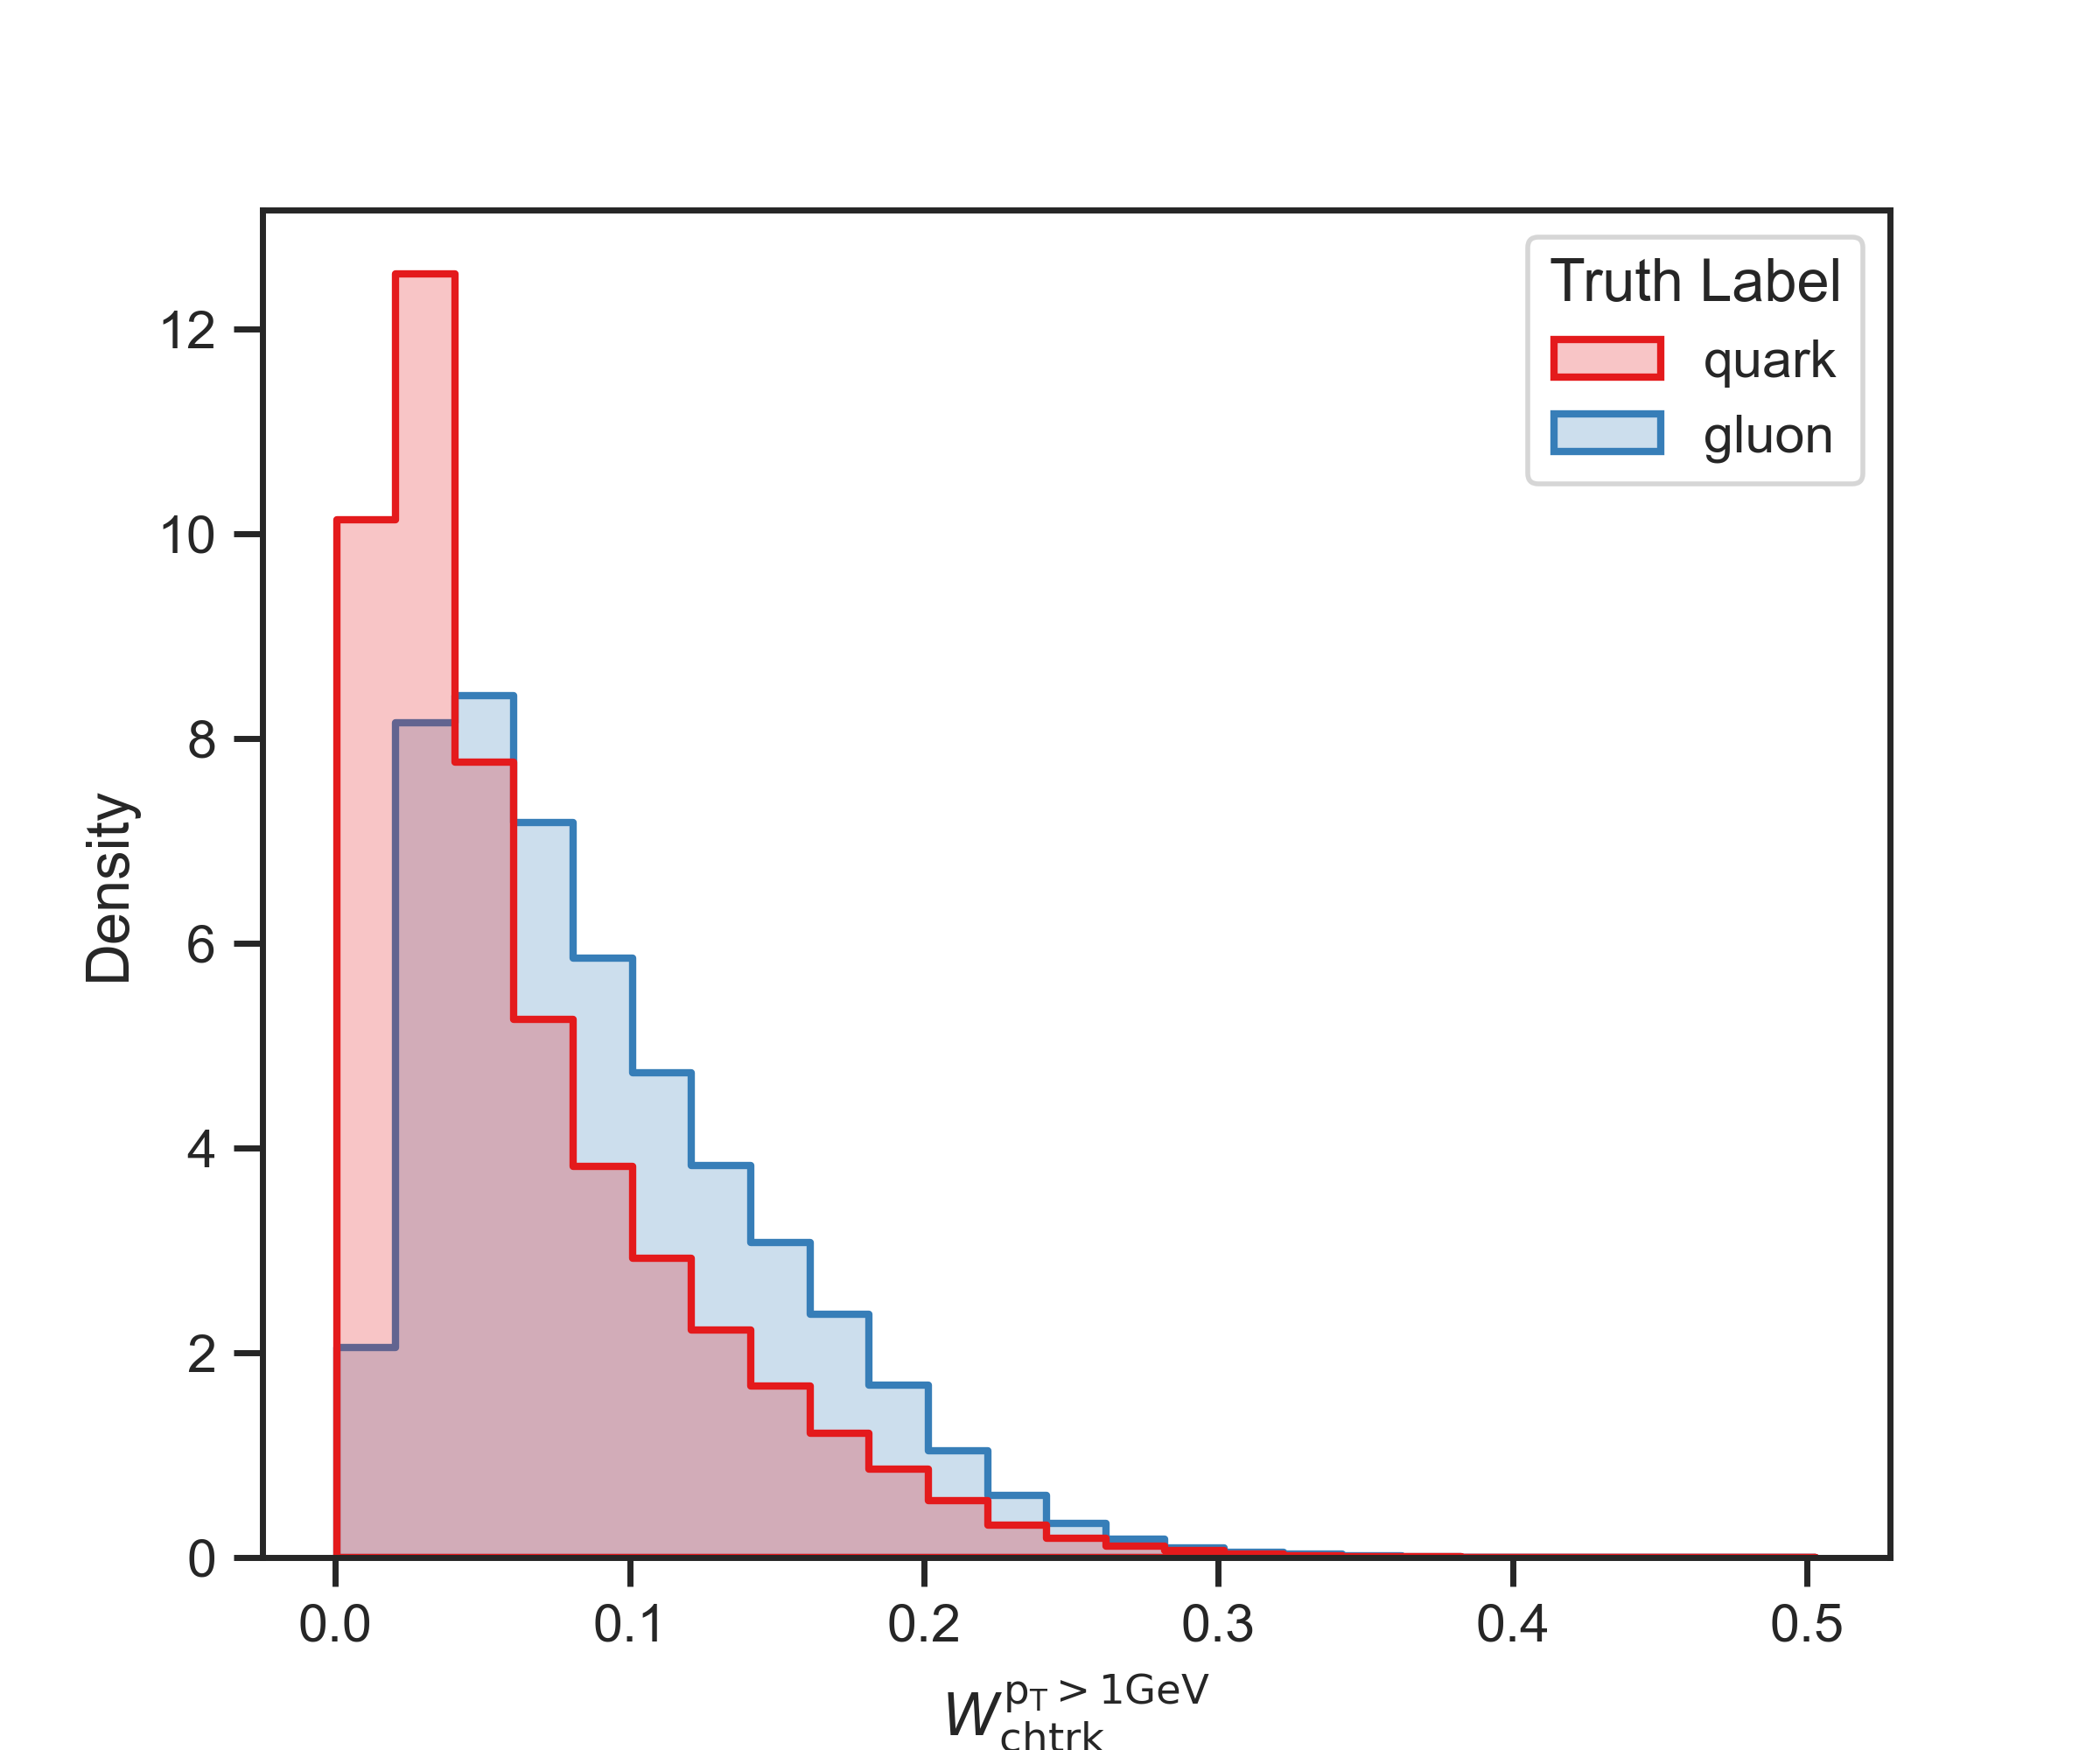
\includegraphics[width=1\textwidth]{src/plots/distributions/highlevel/jets_TrackWidthPt1000[0].png}
		\caption{\texttt{jets\_TrackWidthPt1000[0]}}
		\label{fig:highlevel_20}
	\end{subfigure}
	\begin{subfigure}[t]{0.49\textwidth}
		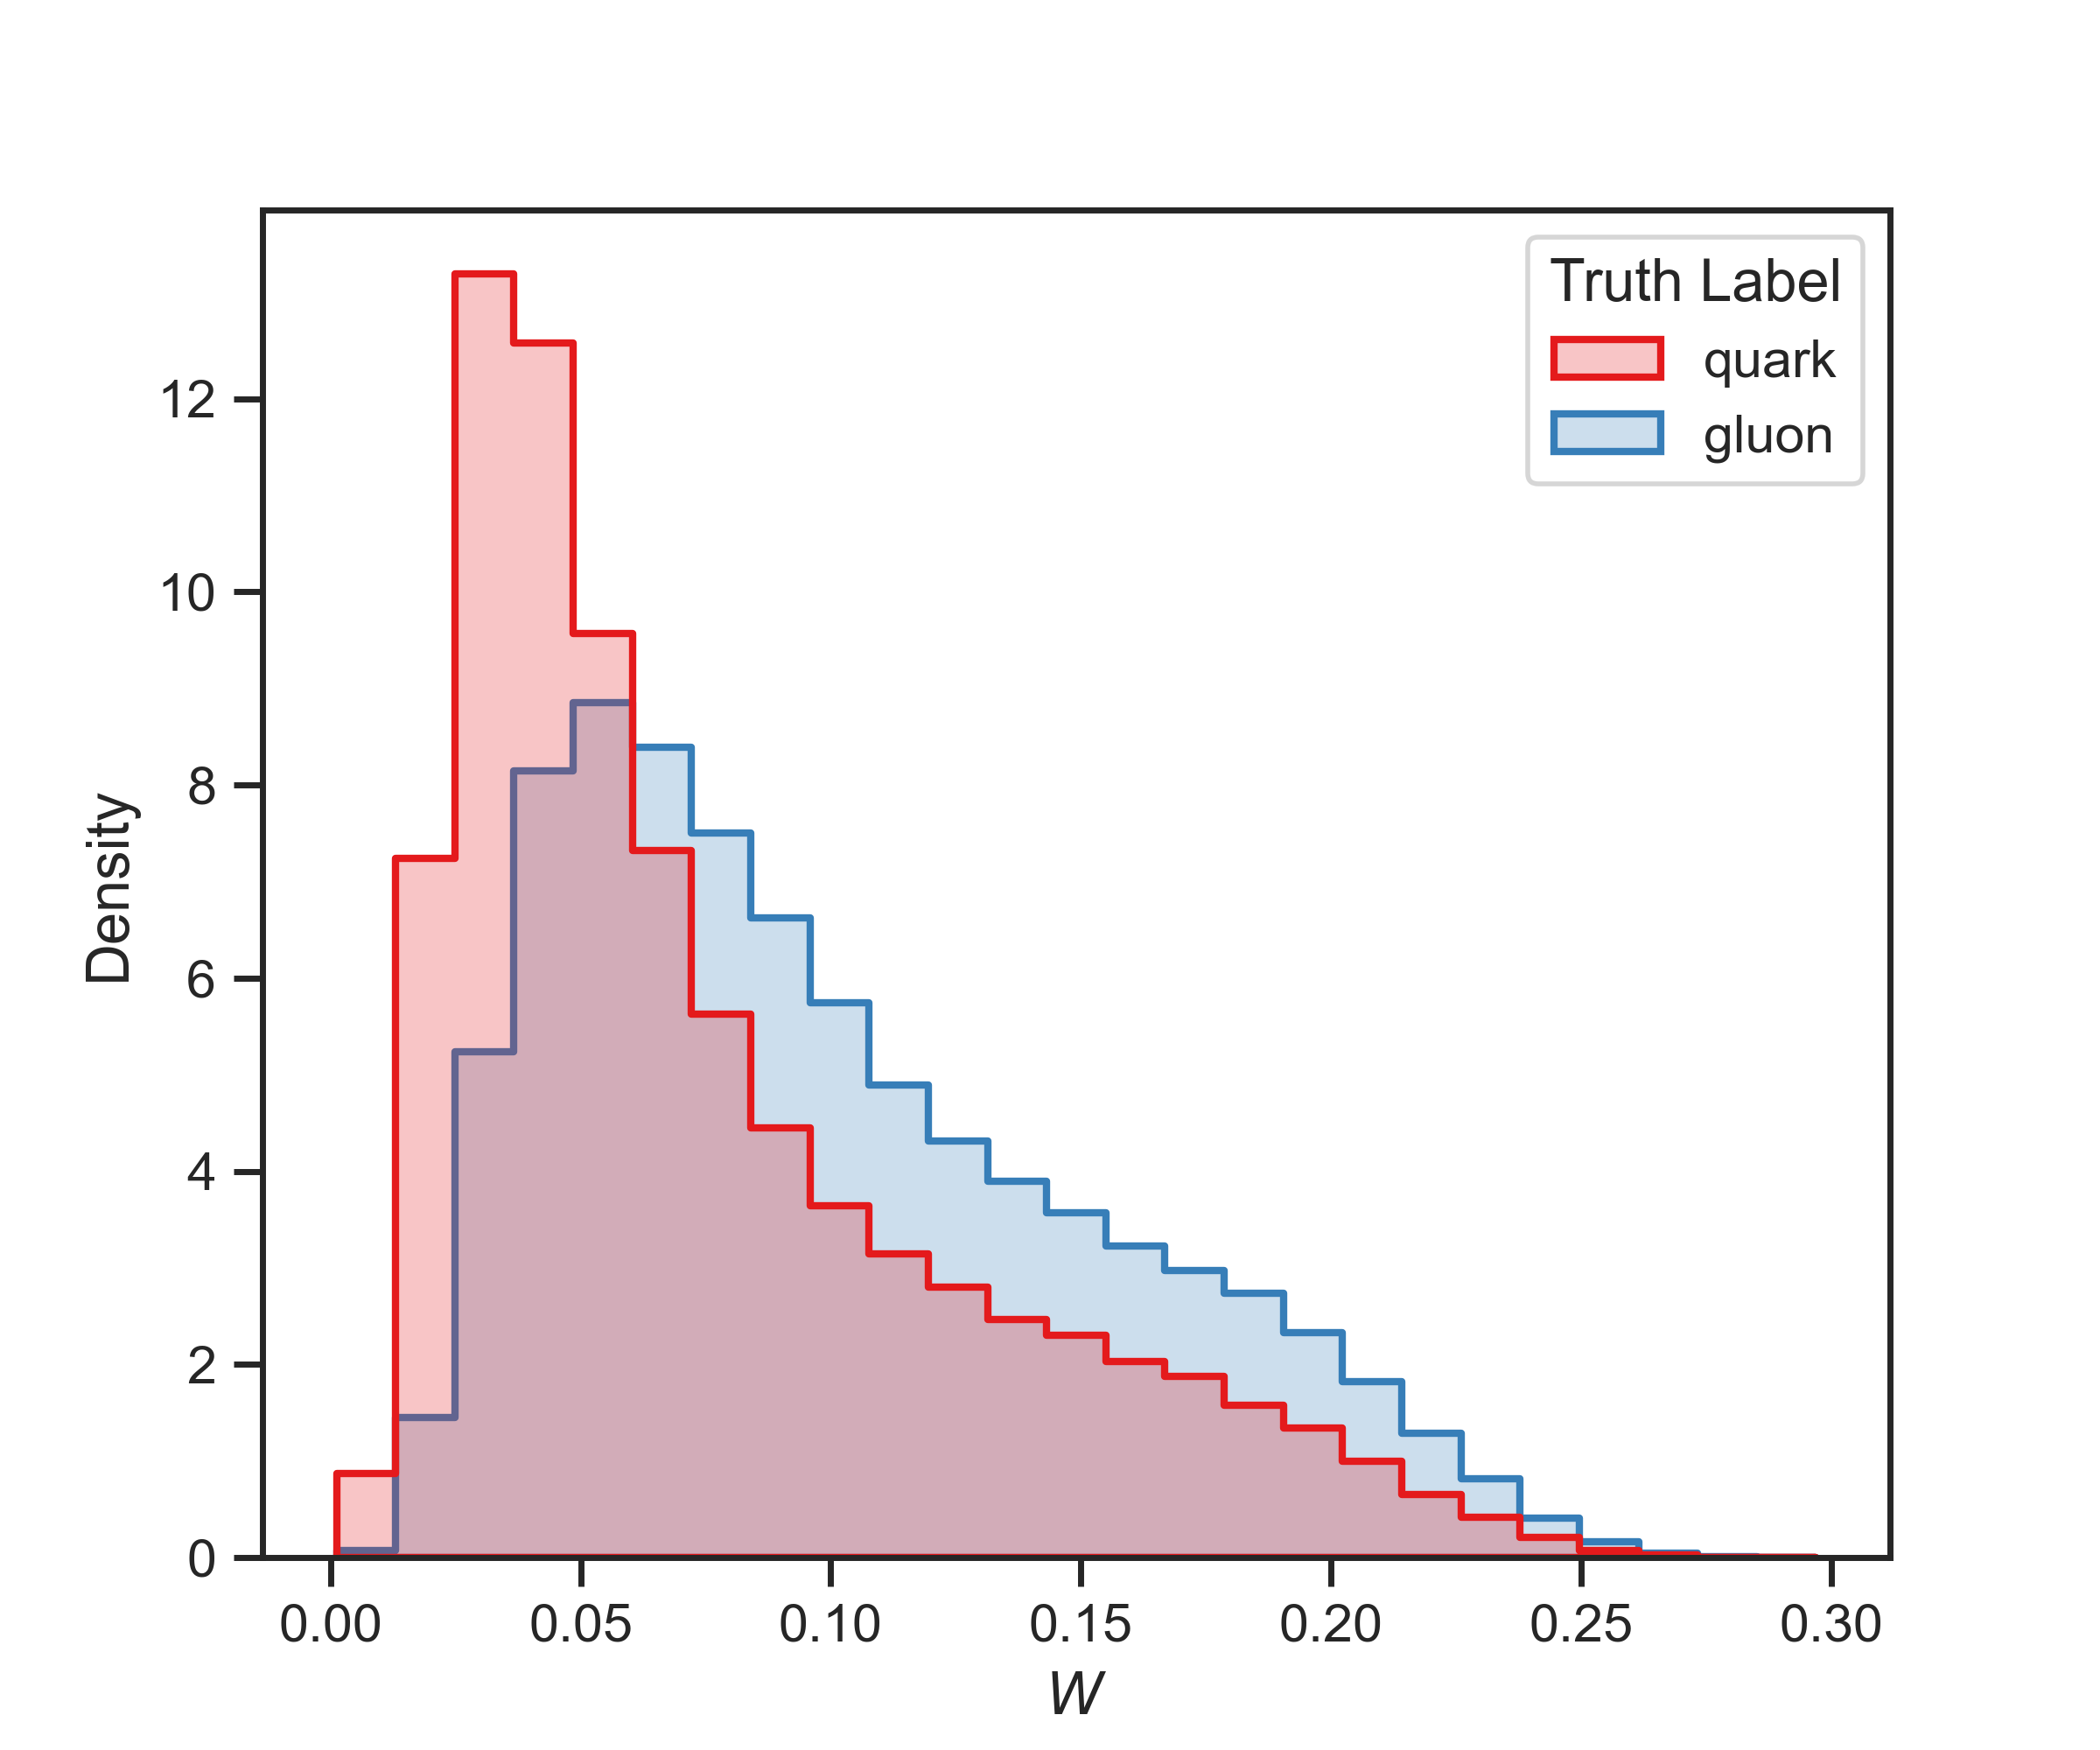
\includegraphics[width=1\textwidth]{src/plots/distributions/highlevel/jets_Width.png}
		\caption{\texttt{jets\_Width}}
		\label{fig:highlevel_21}
	\end{subfigure}
	\begin{subfigure}[t]{0.49\textwidth}
		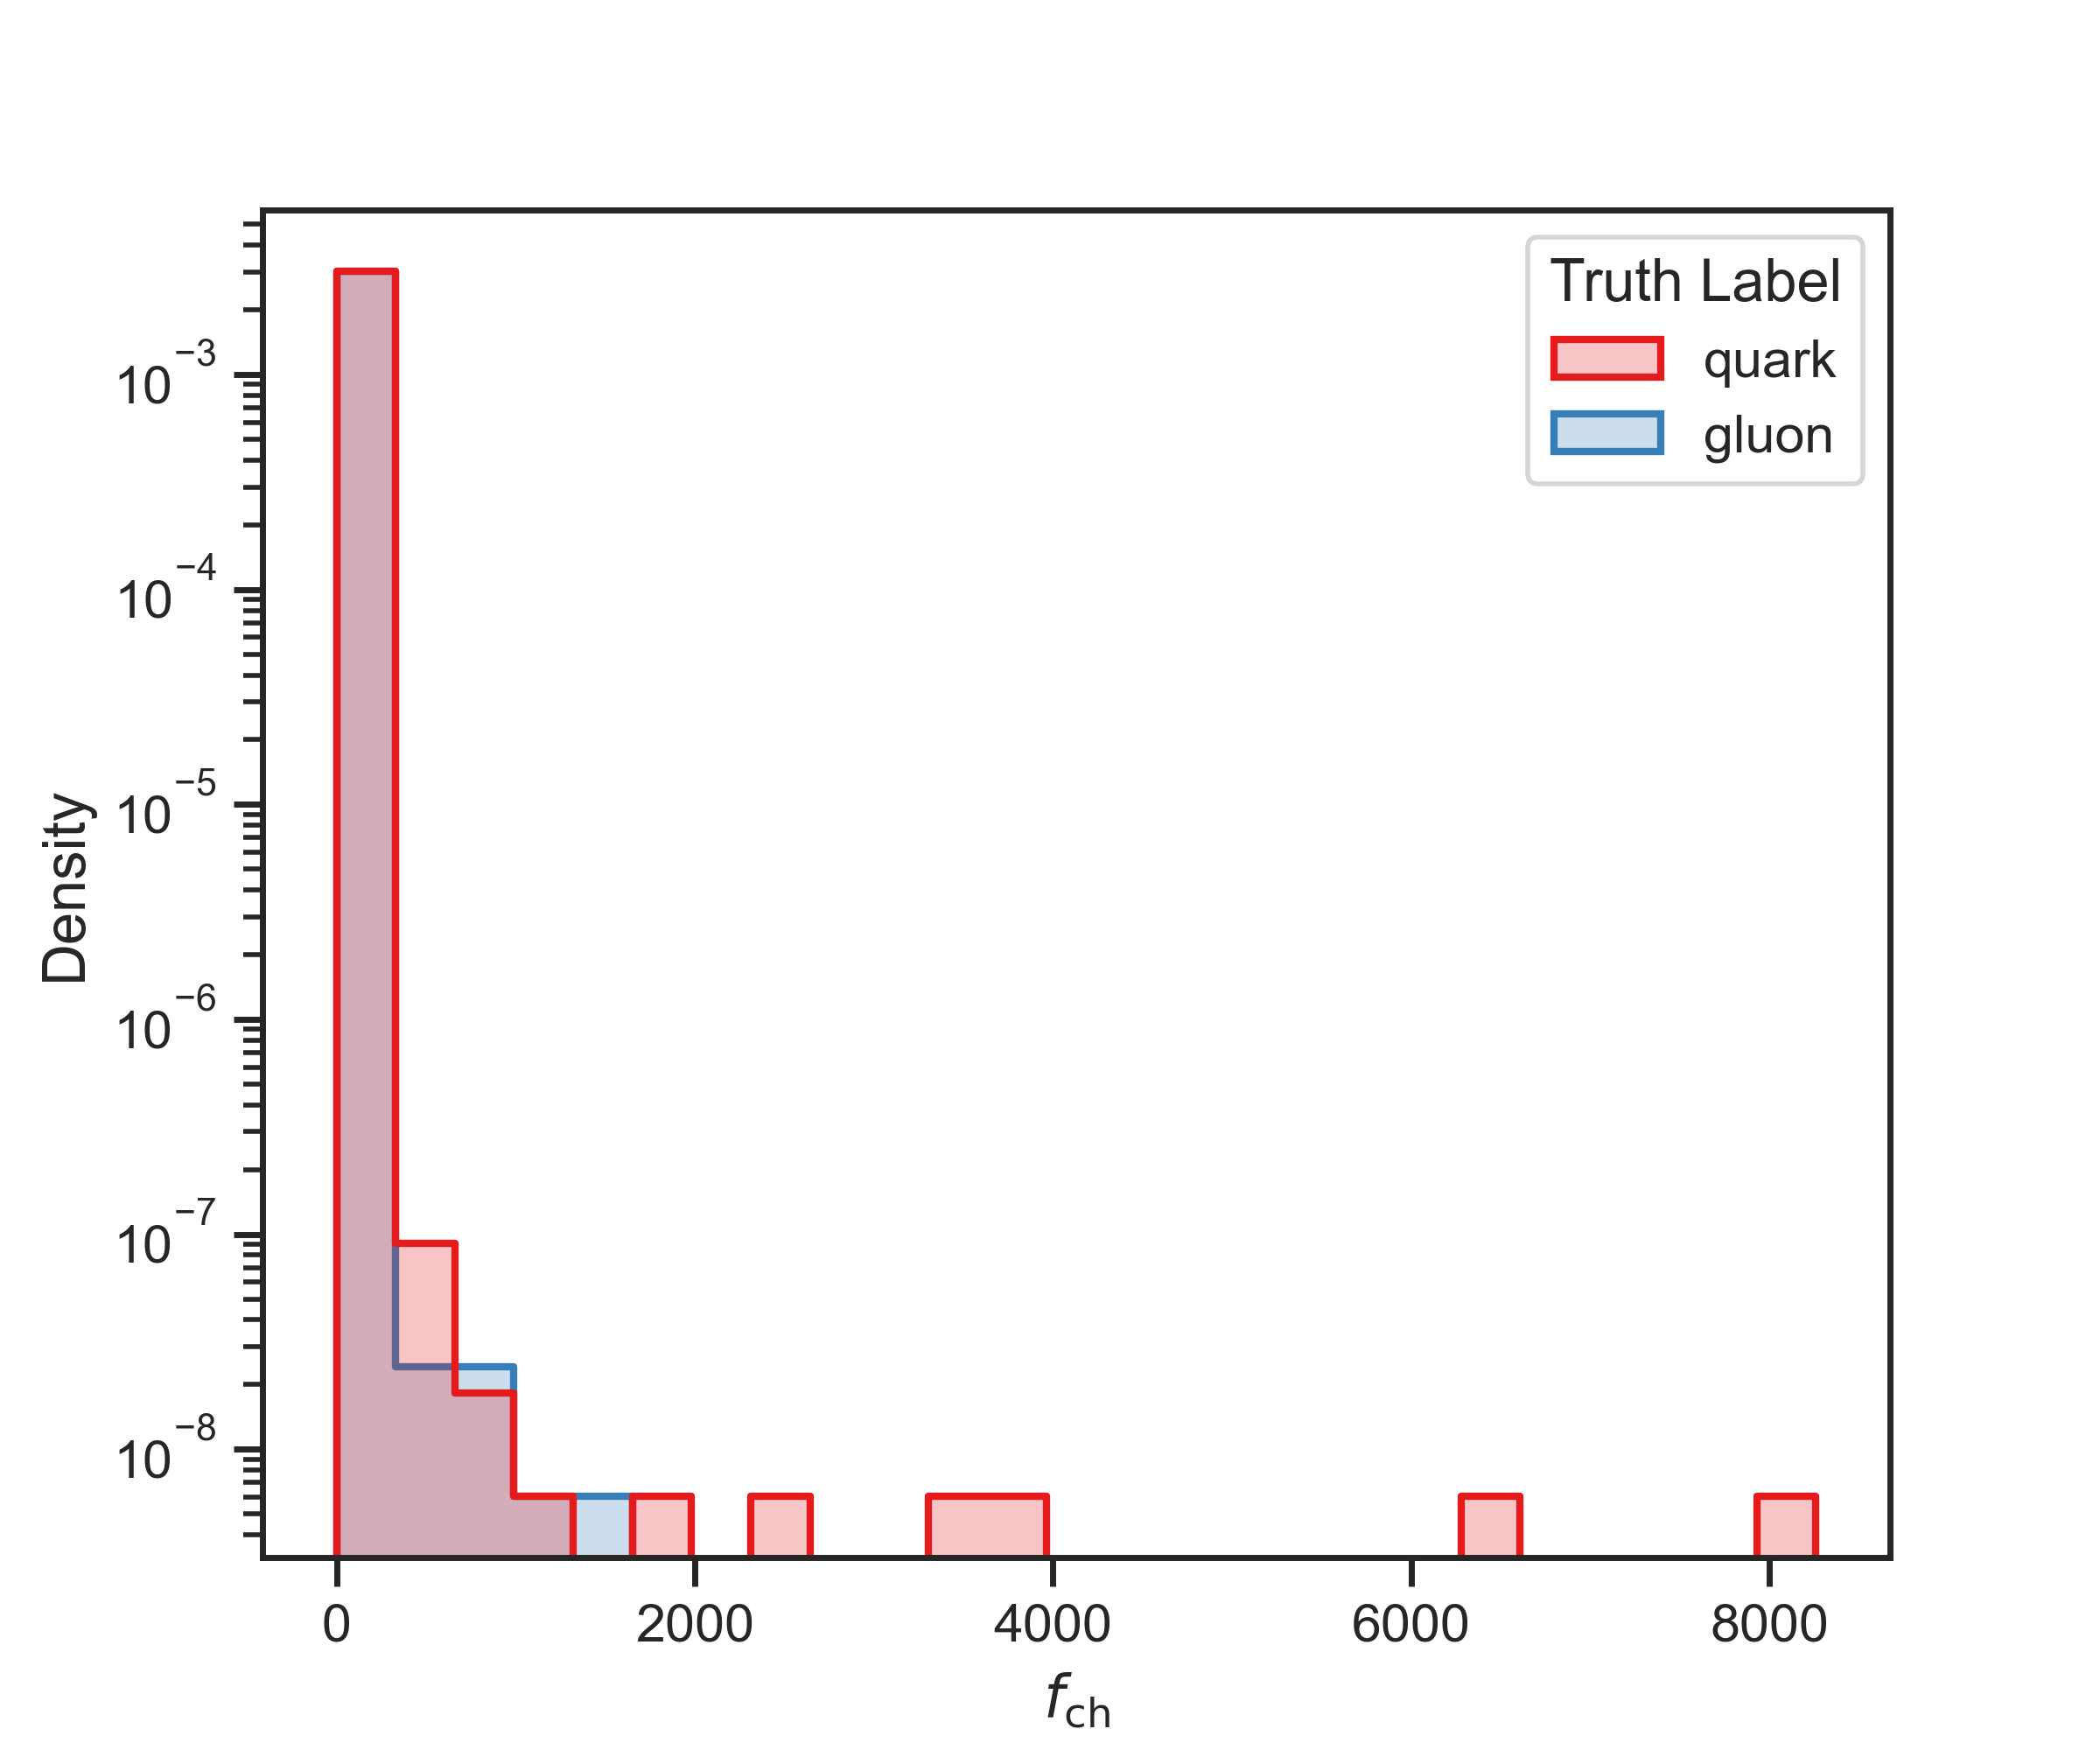
\includegraphics[width=1\textwidth]{src/plots/distributions/highlevel/jets_chf.png}
		\caption{\texttt{jets\_chf}}
		\label{fig:highlevel_22}
	\end{subfigure}
	\begin{subfigure}[t]{0.49\textwidth}
		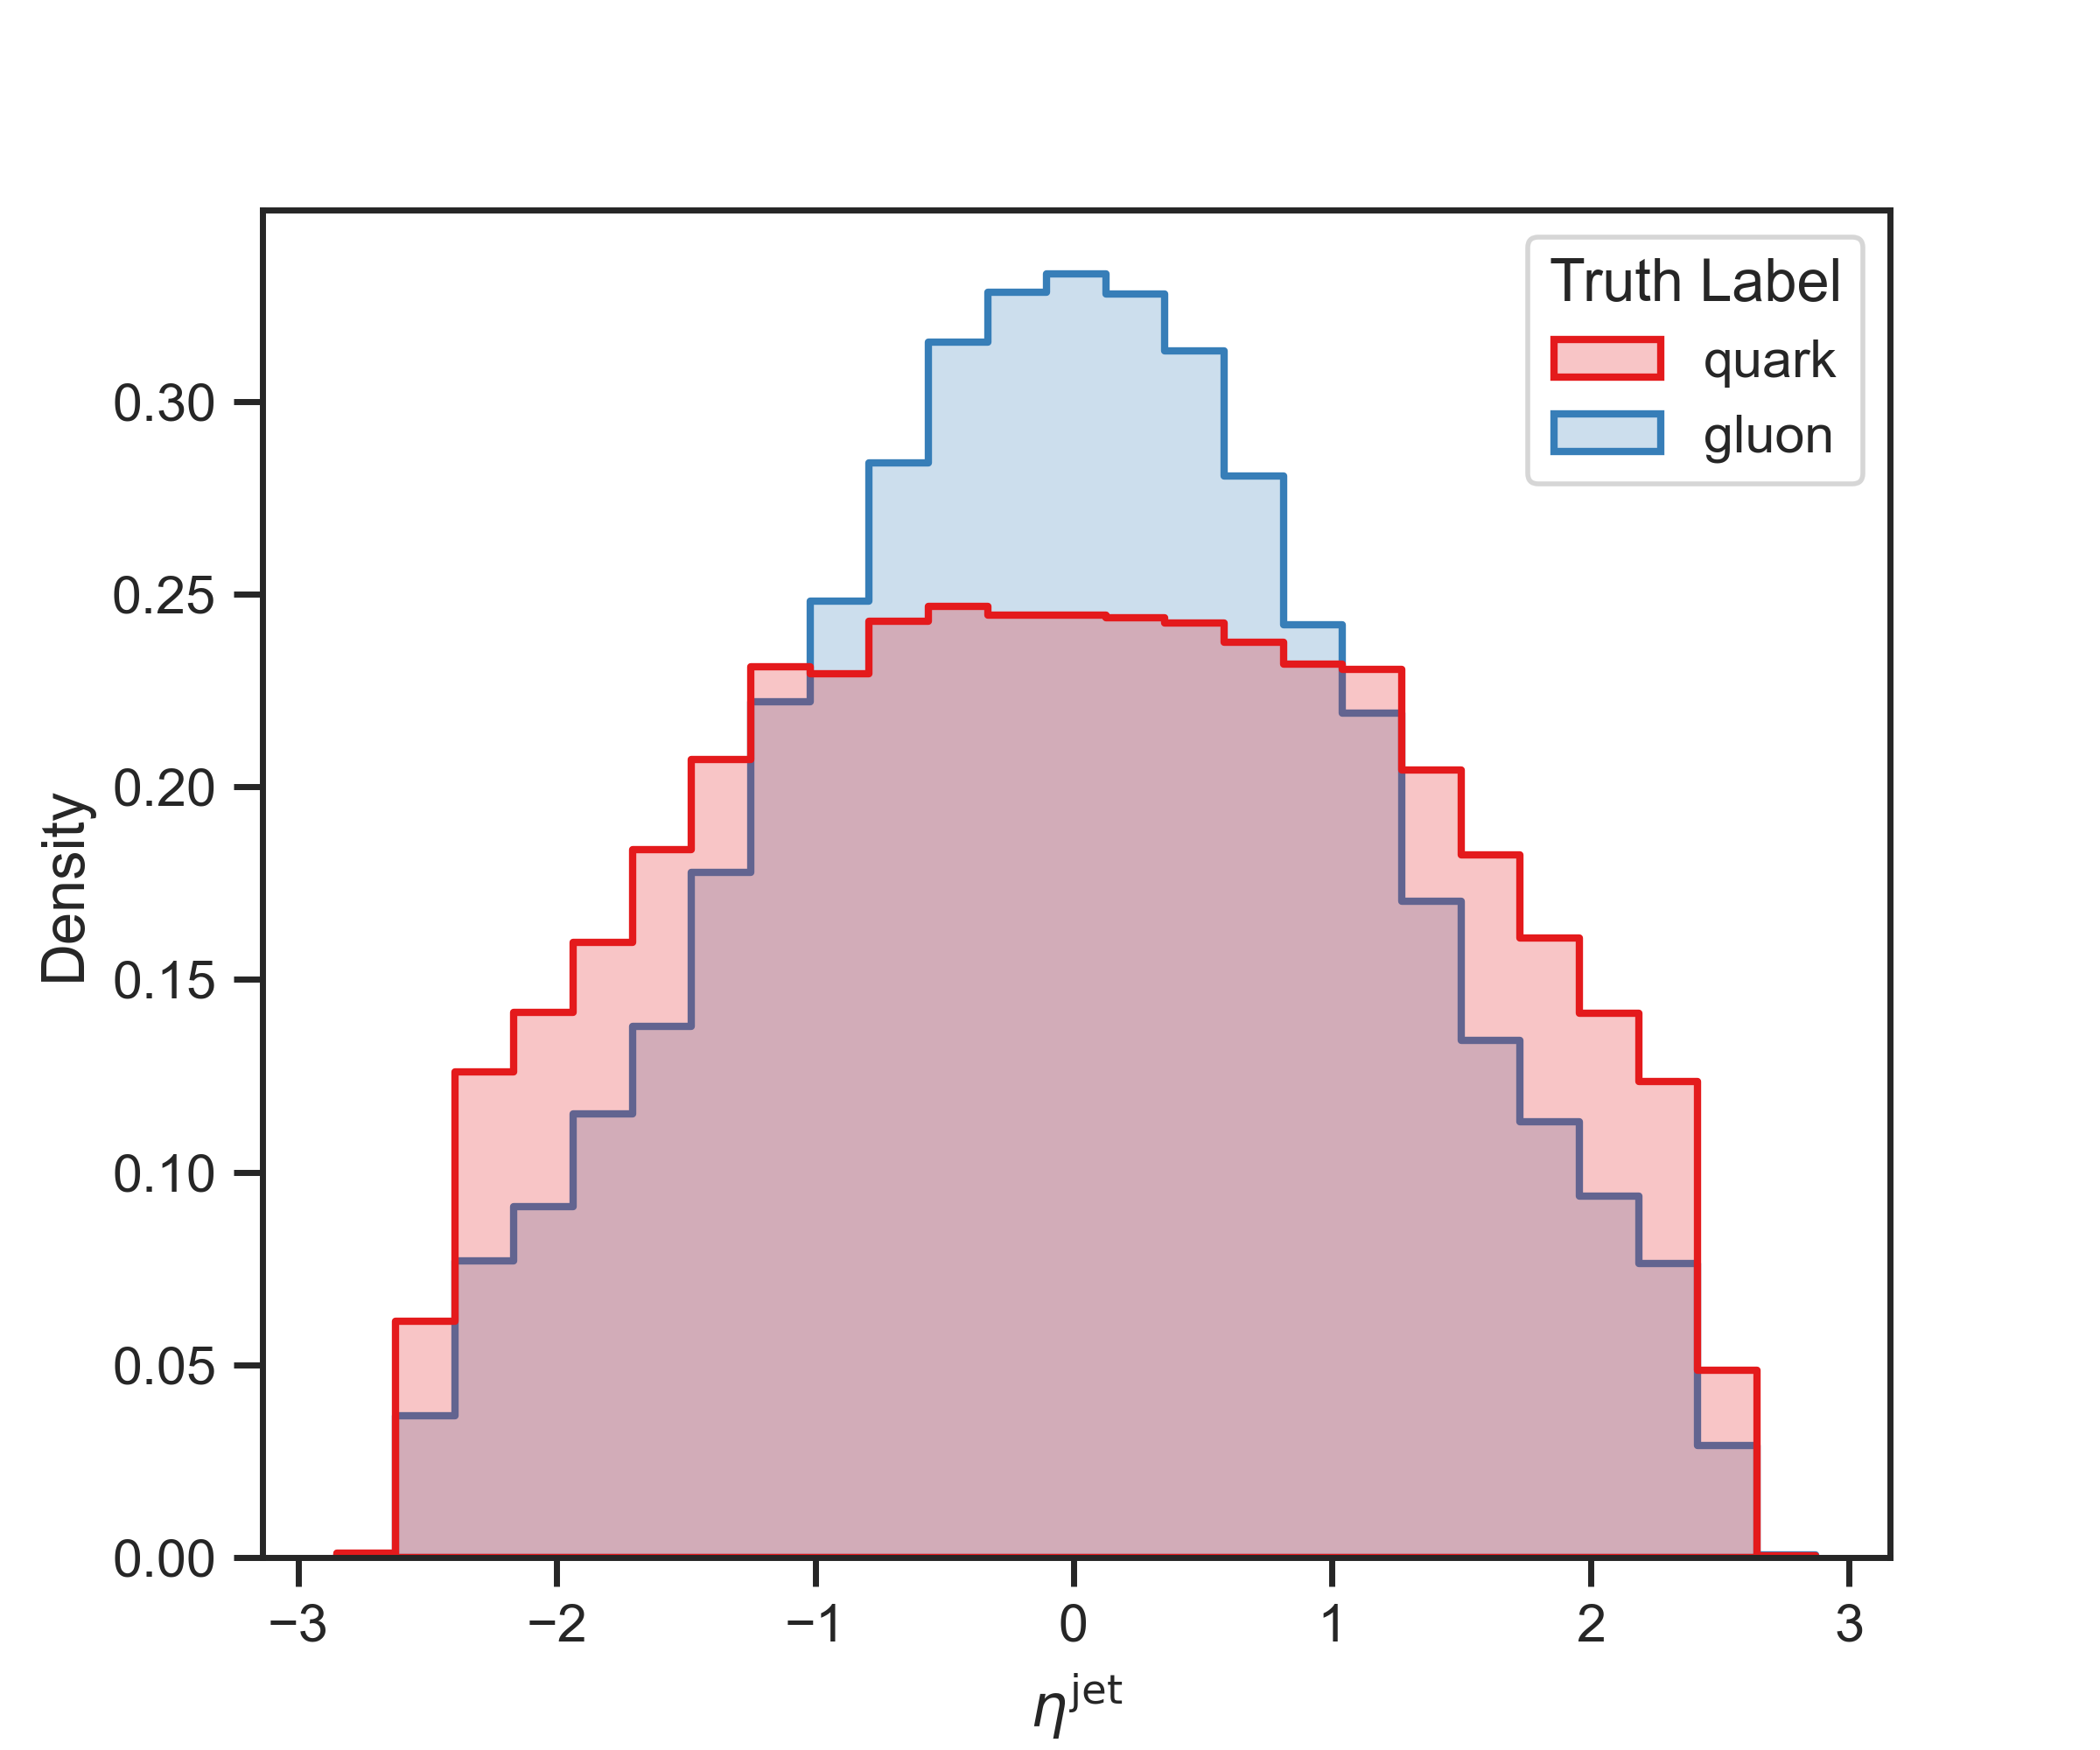
\includegraphics[width=1\textwidth]{src/plots/distributions/highlevel/jets_eta.png}
		\caption{\texttt{jets\_eta}}
		\label{fig:highlevel_23}
	\end{subfigure}
\caption{High-level Jet Variables, part 4}
\label{fig:highlevel_18-23}
\end{figure}

\begin{figure}[!htb]
	\centering
	\begin{subfigure}[t]{0.49\textwidth}
		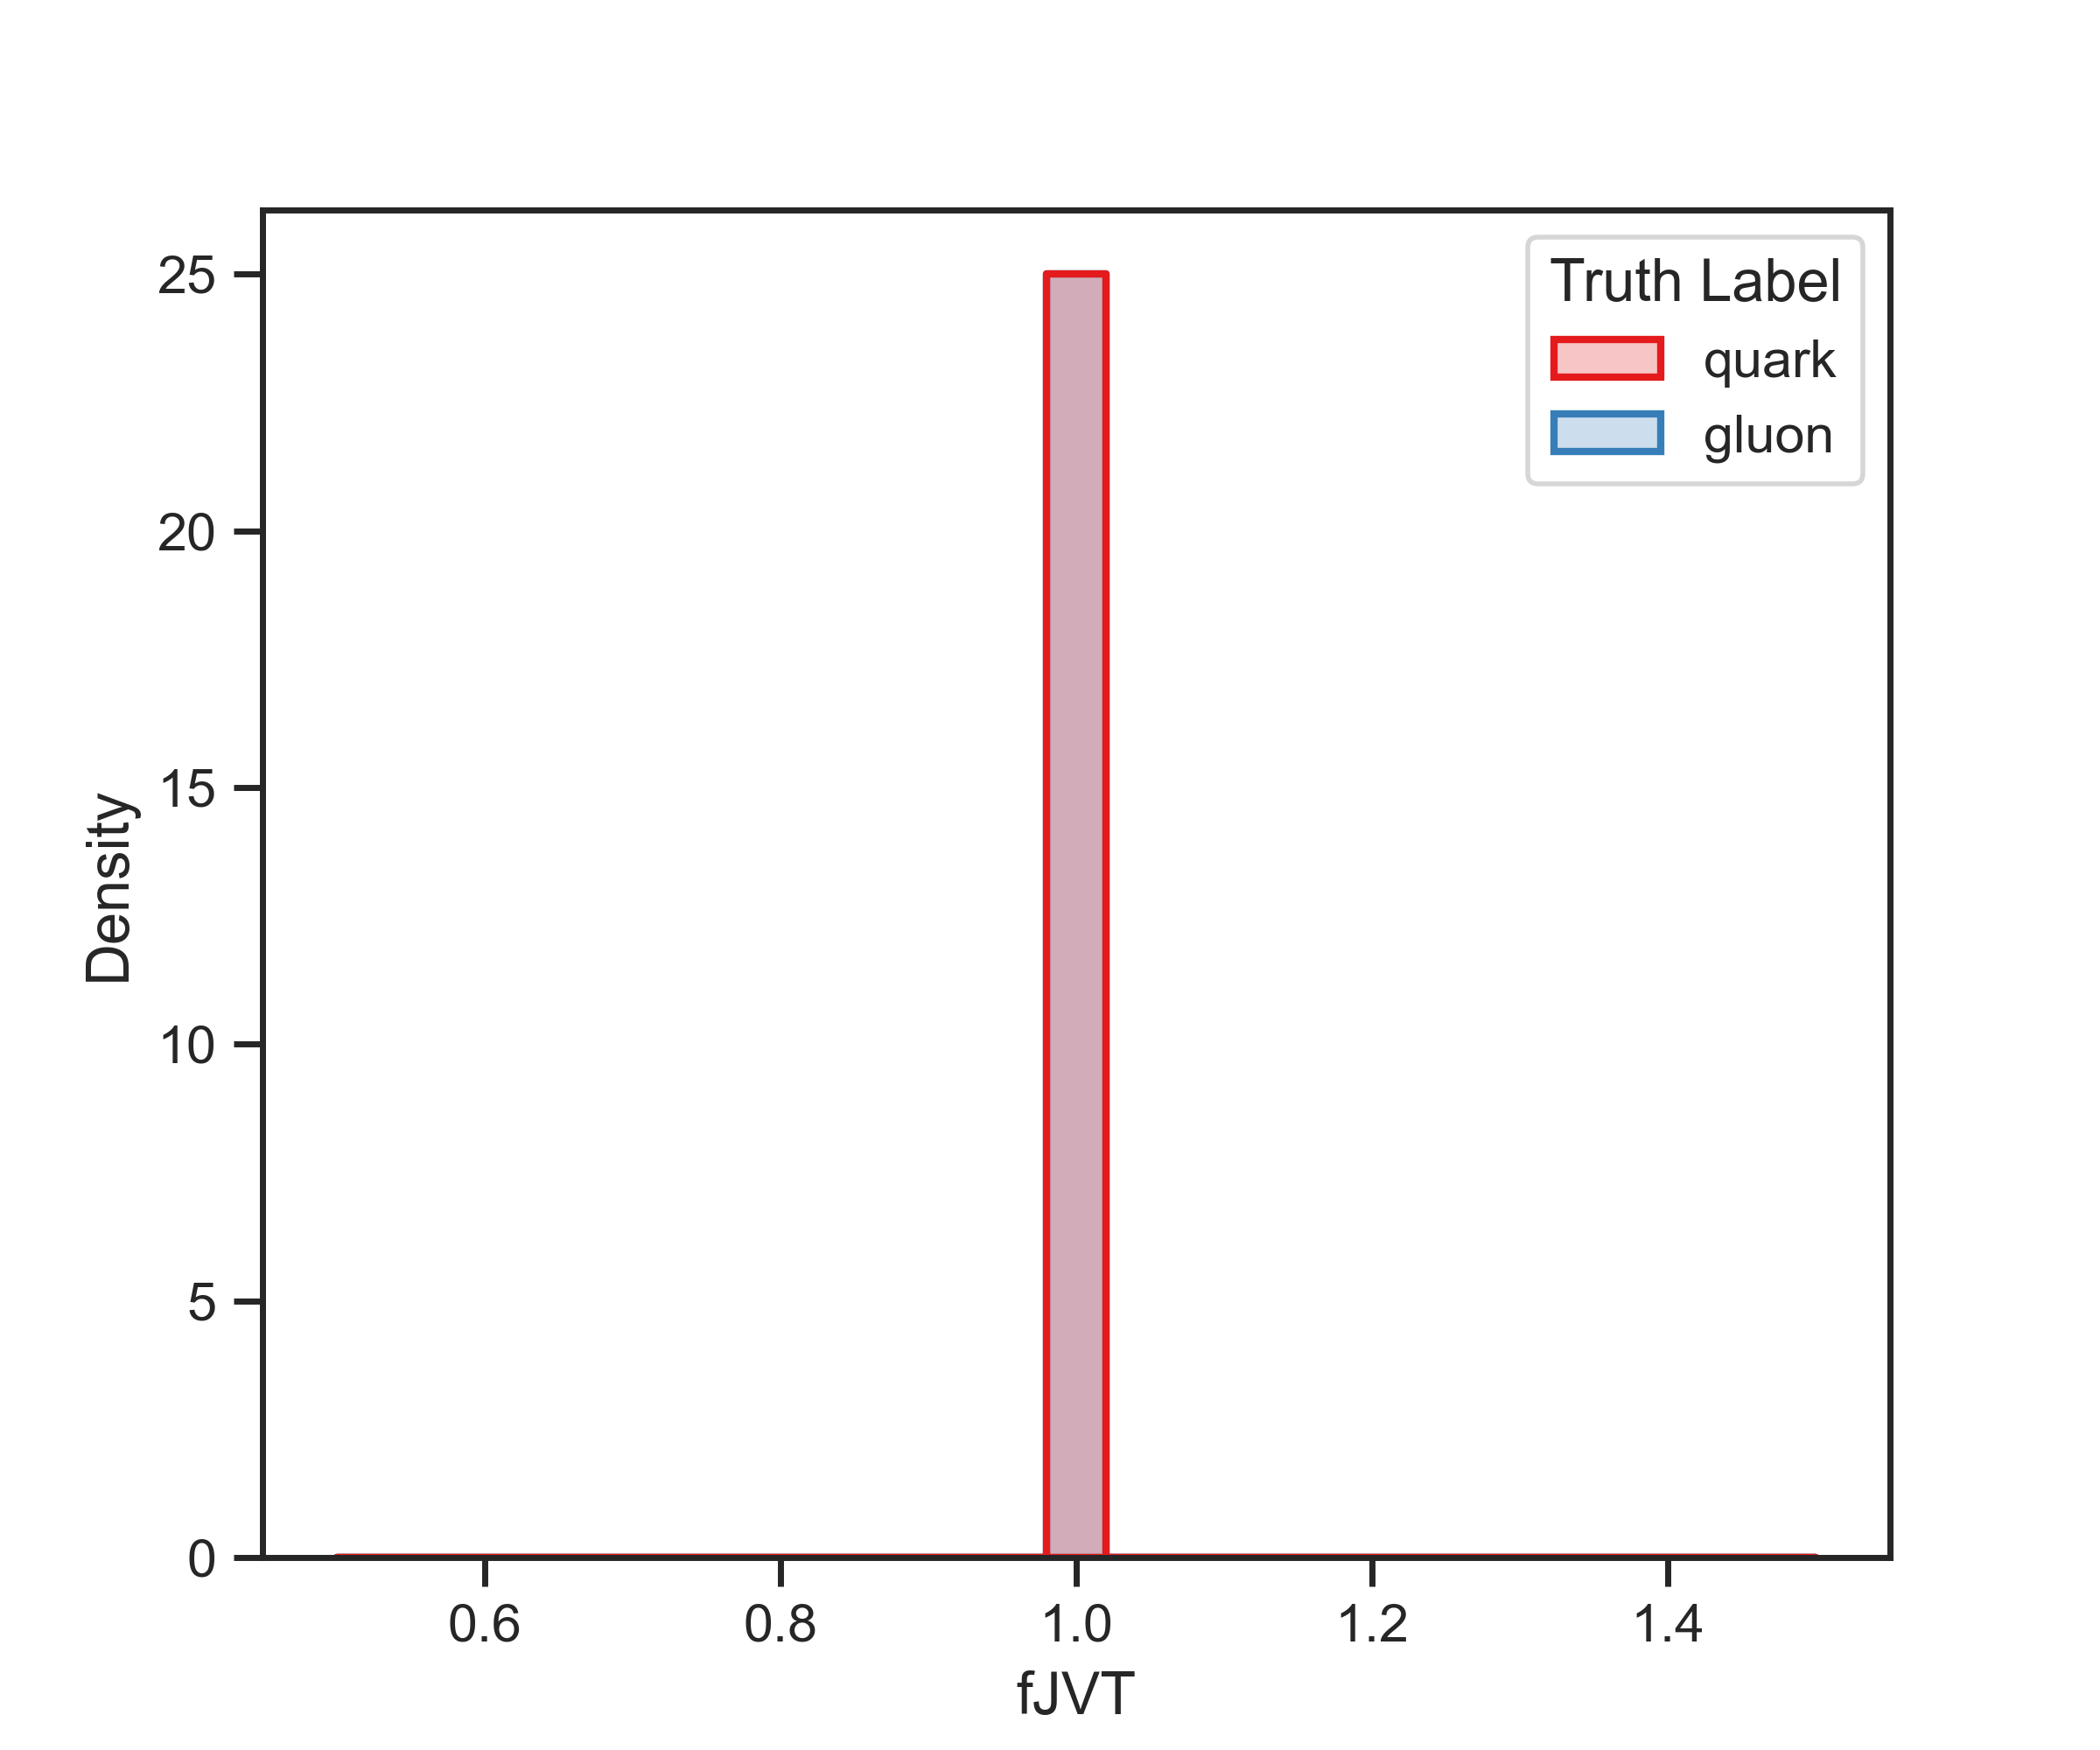
\includegraphics[width=1\textwidth]{src/plots/distributions/highlevel/jets_fJVT.png}
		\caption{\texttt{jets\_fJVT}}
		\label{fig:highlevel_24}
	\end{subfigure}
	\begin{subfigure}[t]{0.49\textwidth}
		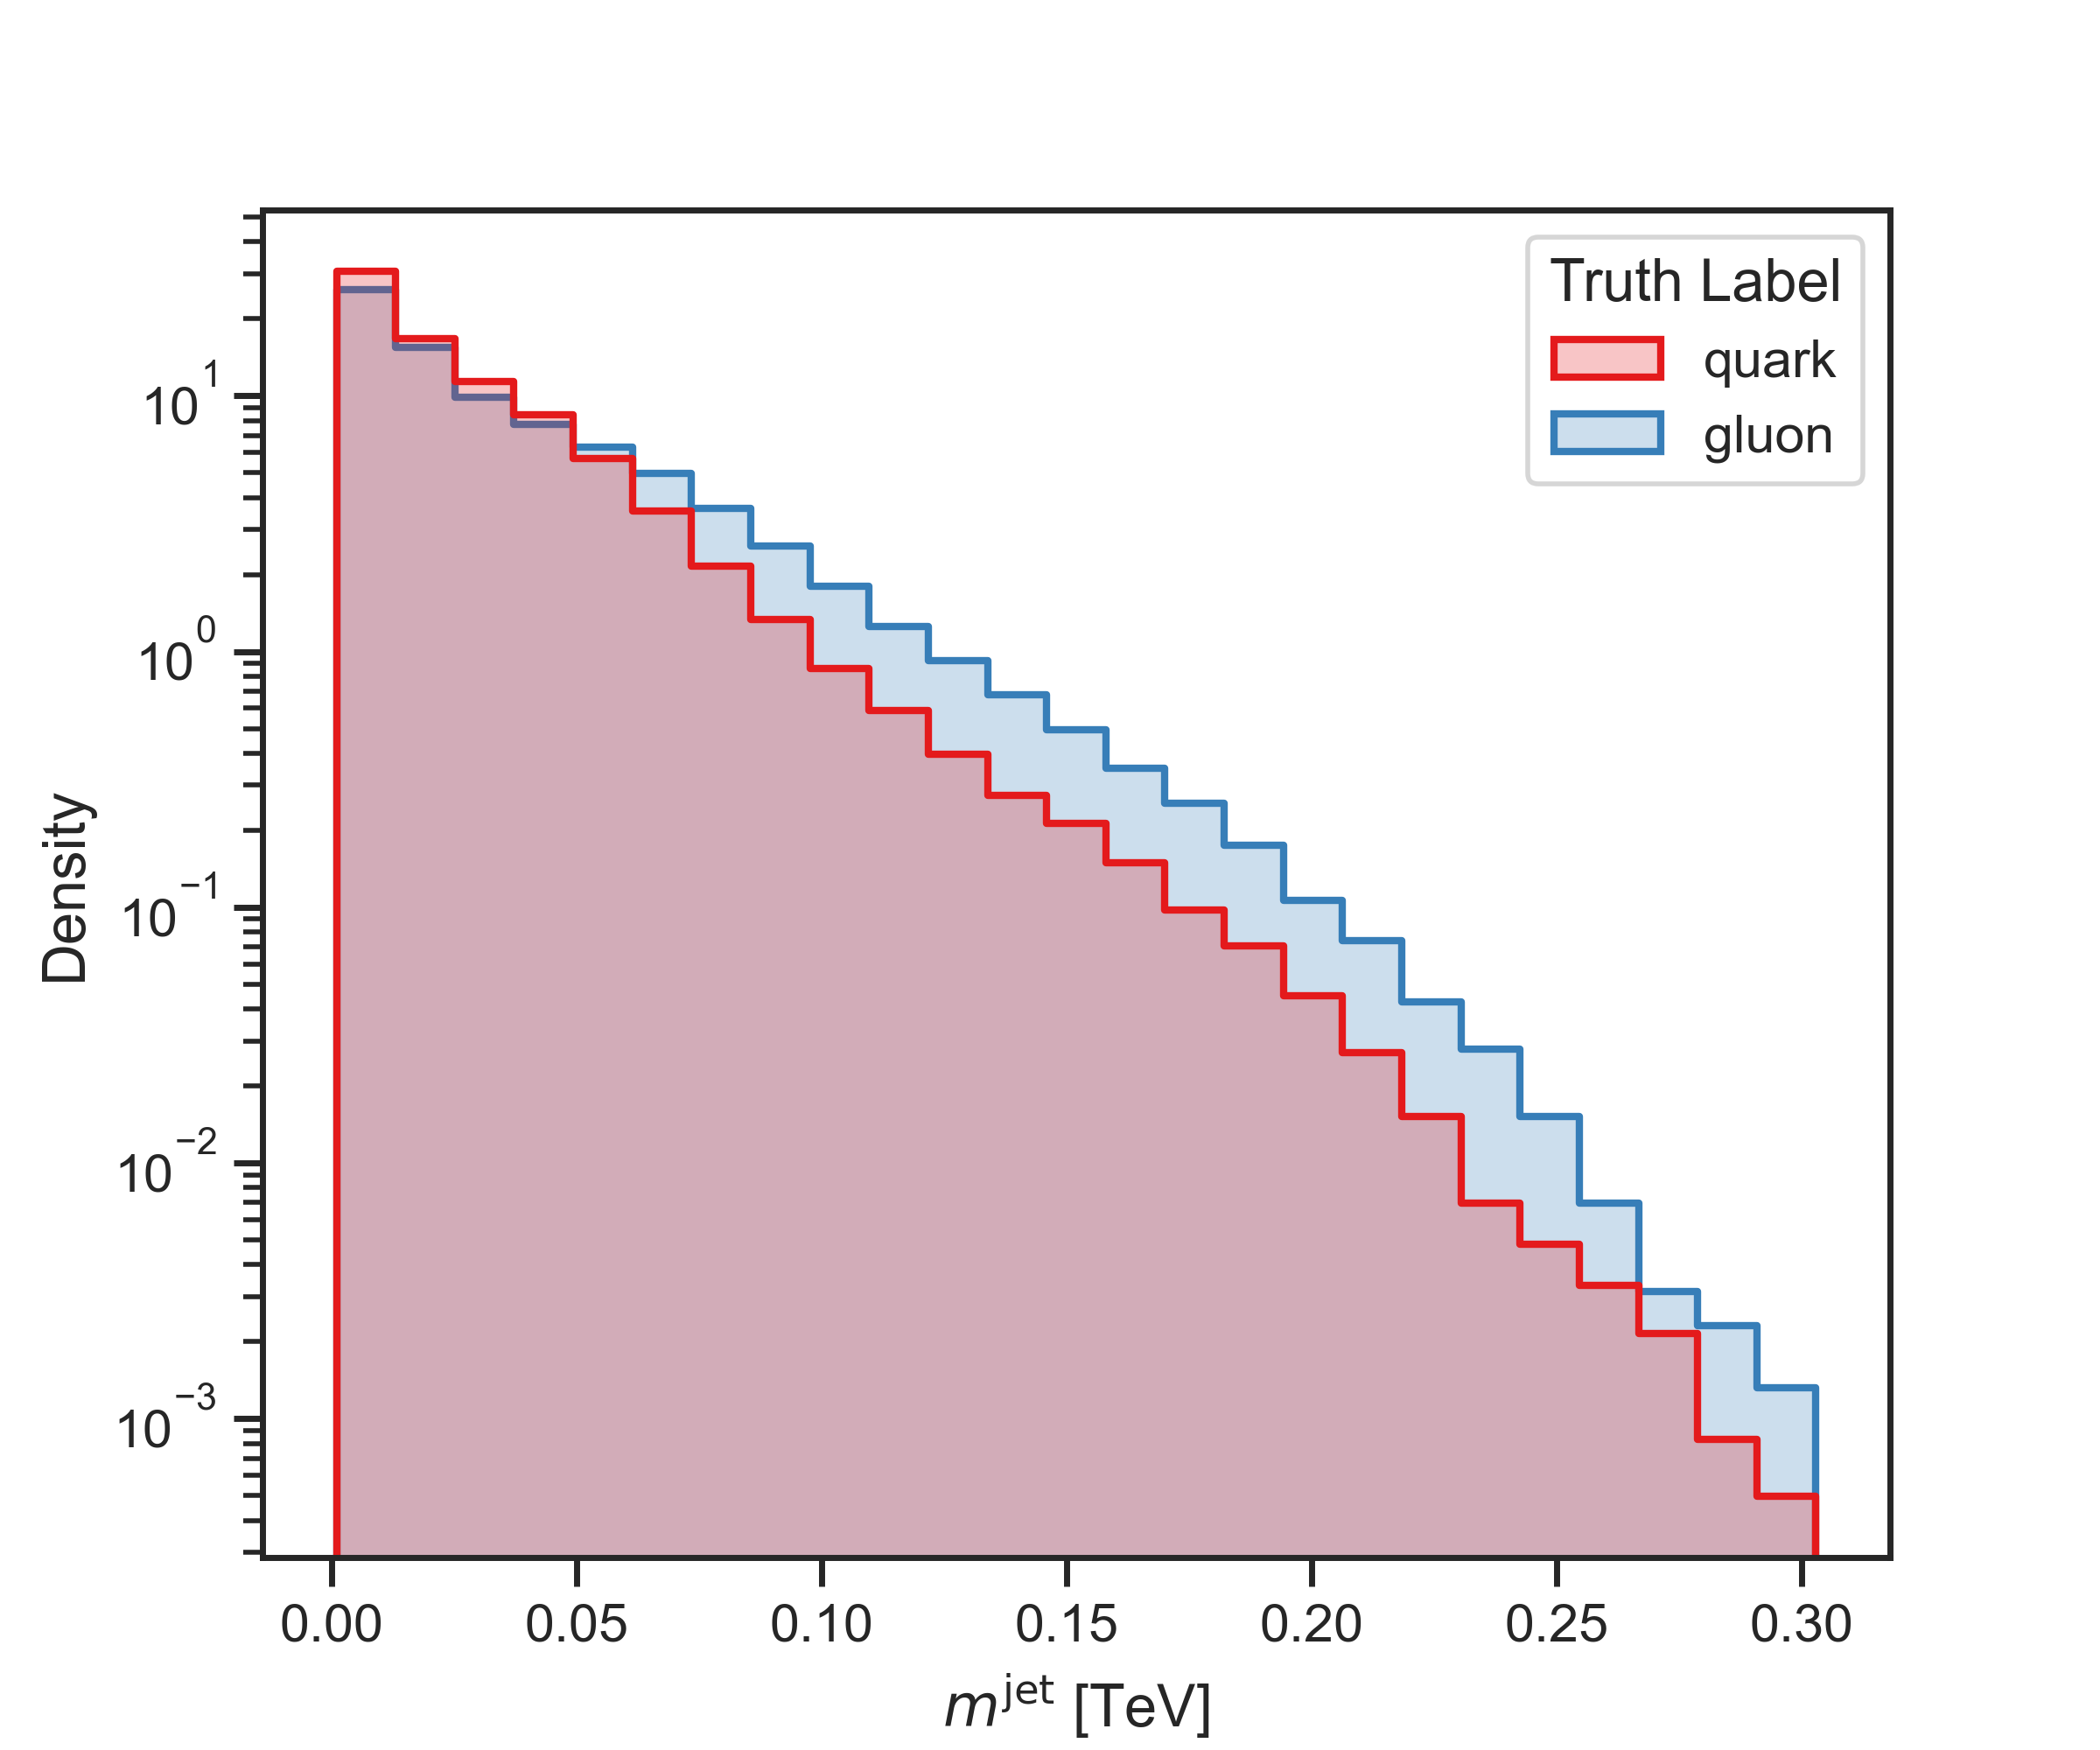
\includegraphics[width=1\textwidth]{src/plots/distributions/highlevel/jets_m.png}
		\caption{\texttt{jets\_m}}
		\label{fig:highlevel_25}
	\end{subfigure}
	\begin{subfigure}[t]{0.49\textwidth}
		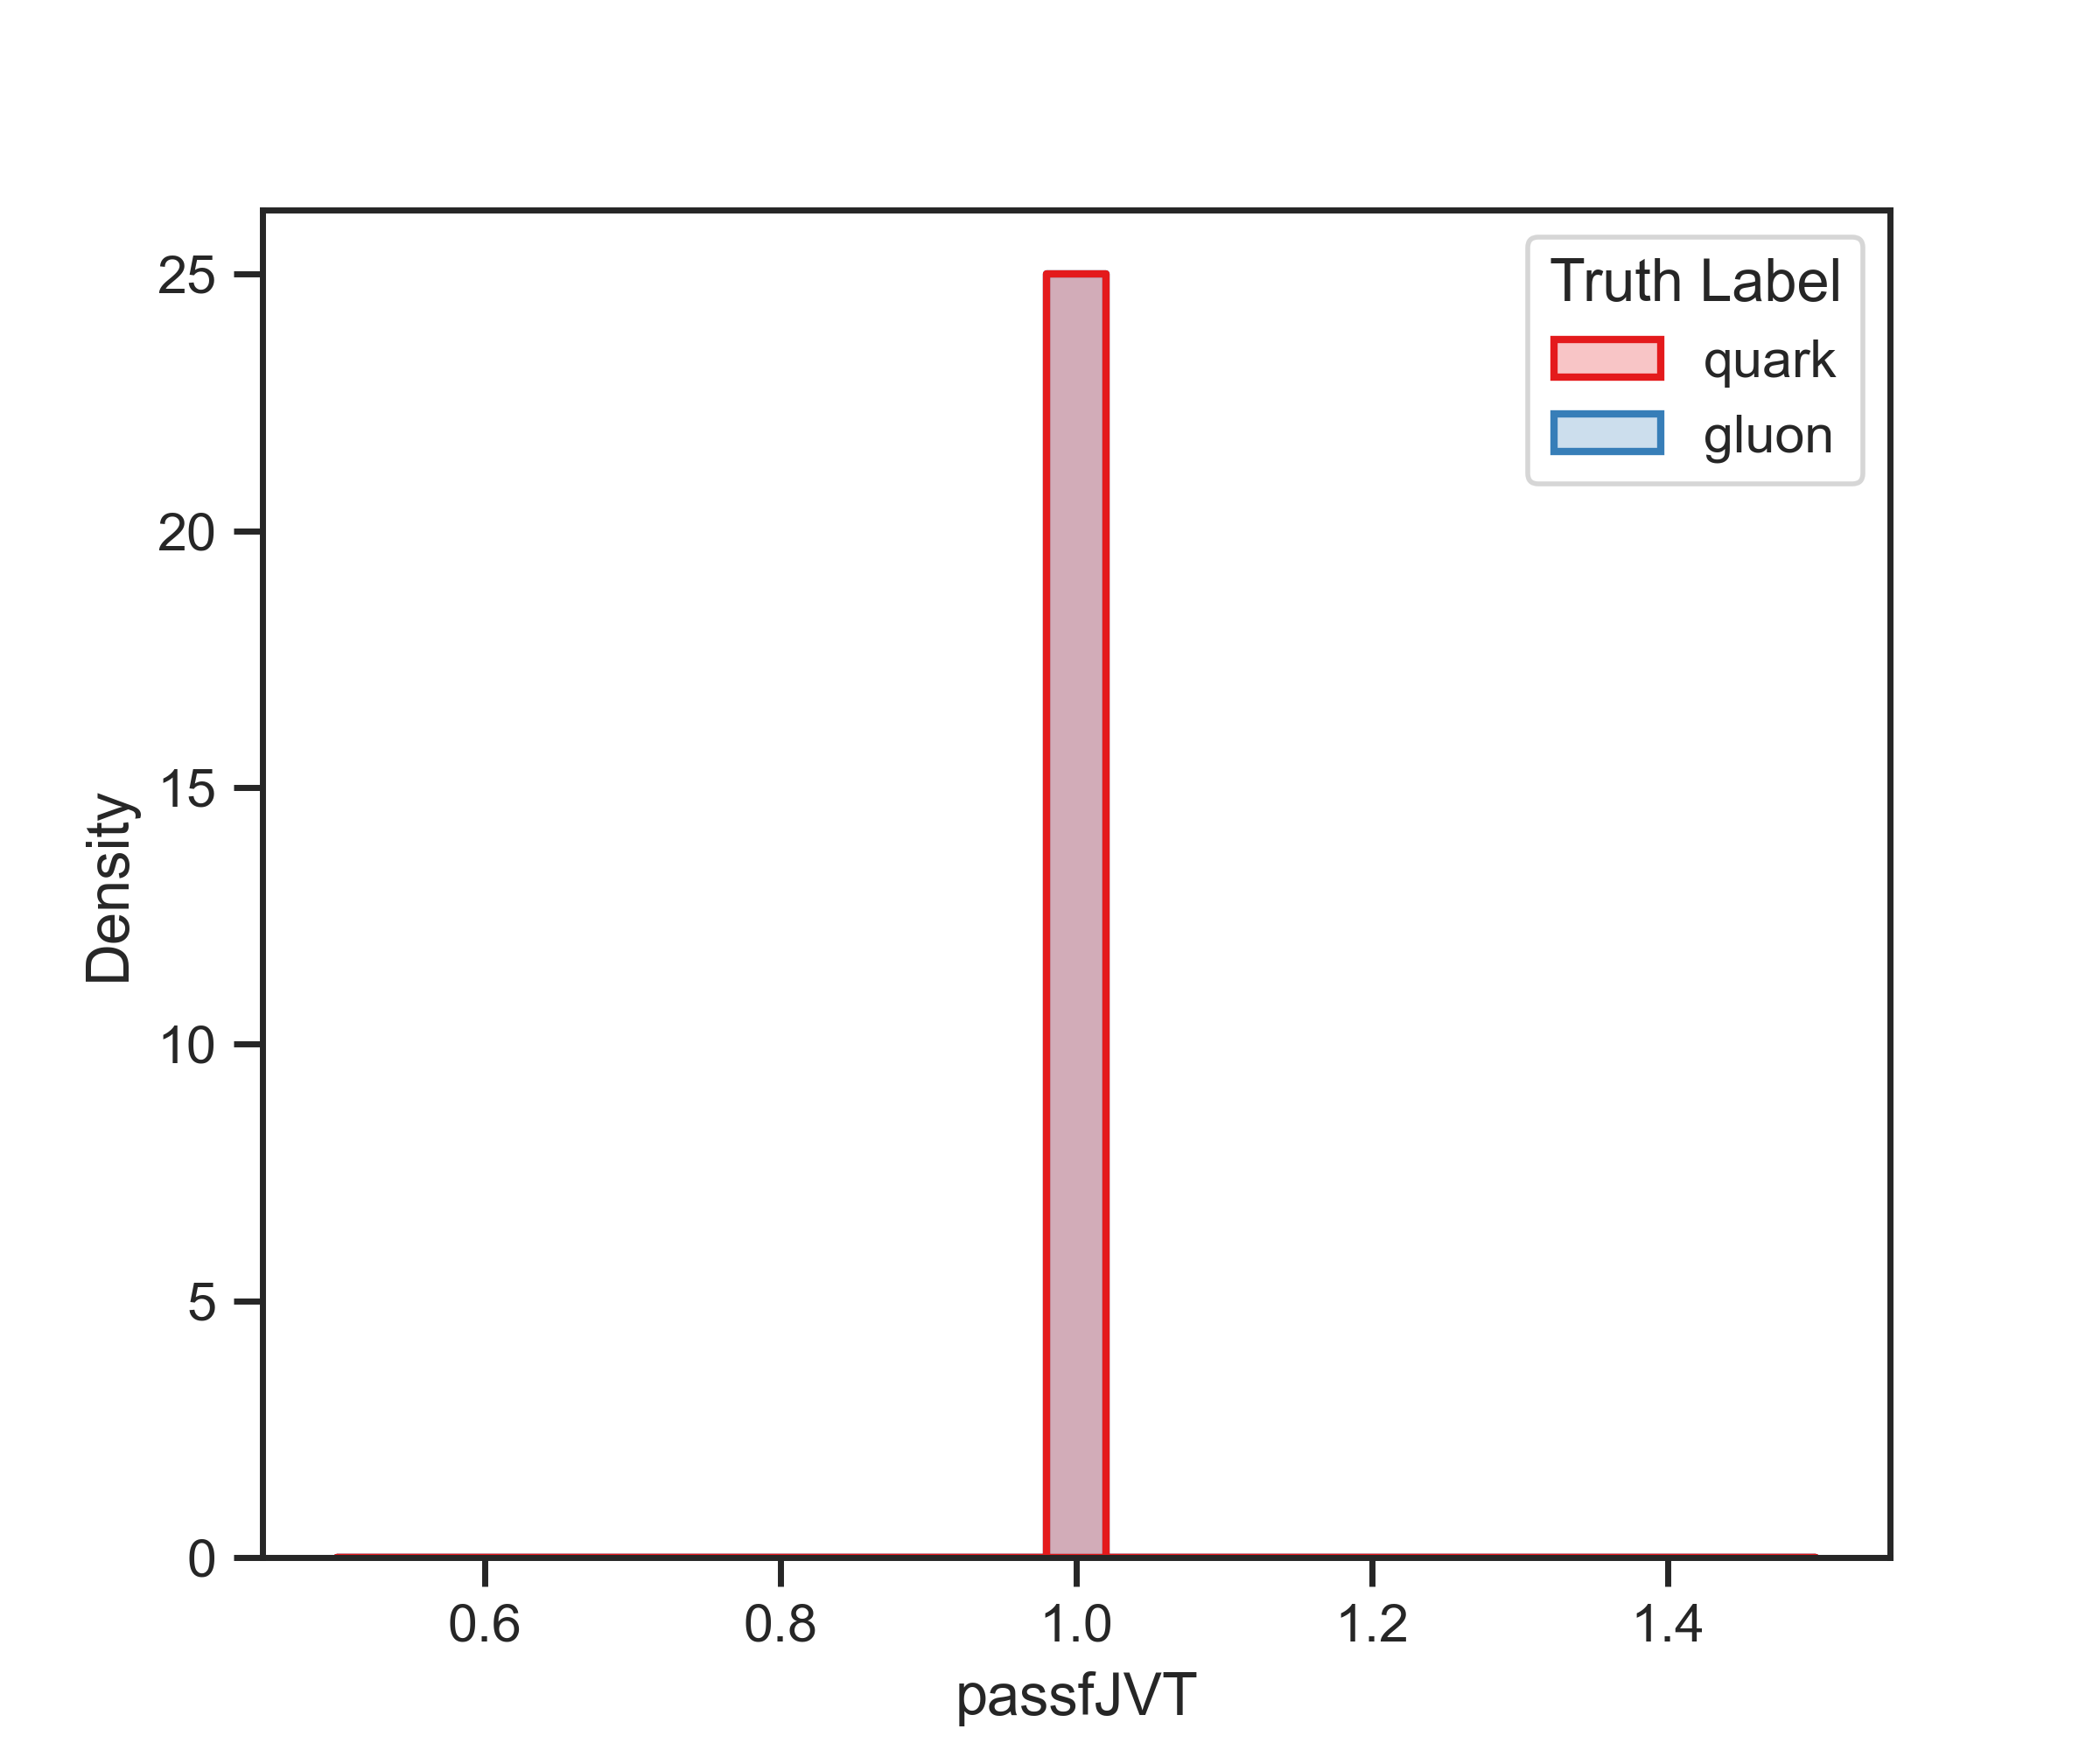
\includegraphics[width=1\textwidth]{src/plots/distributions/highlevel/jets_passFJVT.png}
		\caption{\texttt{jets\_passFJVT}}
		\label{fig:highlevel_26}
	\end{subfigure}
	\begin{subfigure}[t]{0.49\textwidth}
		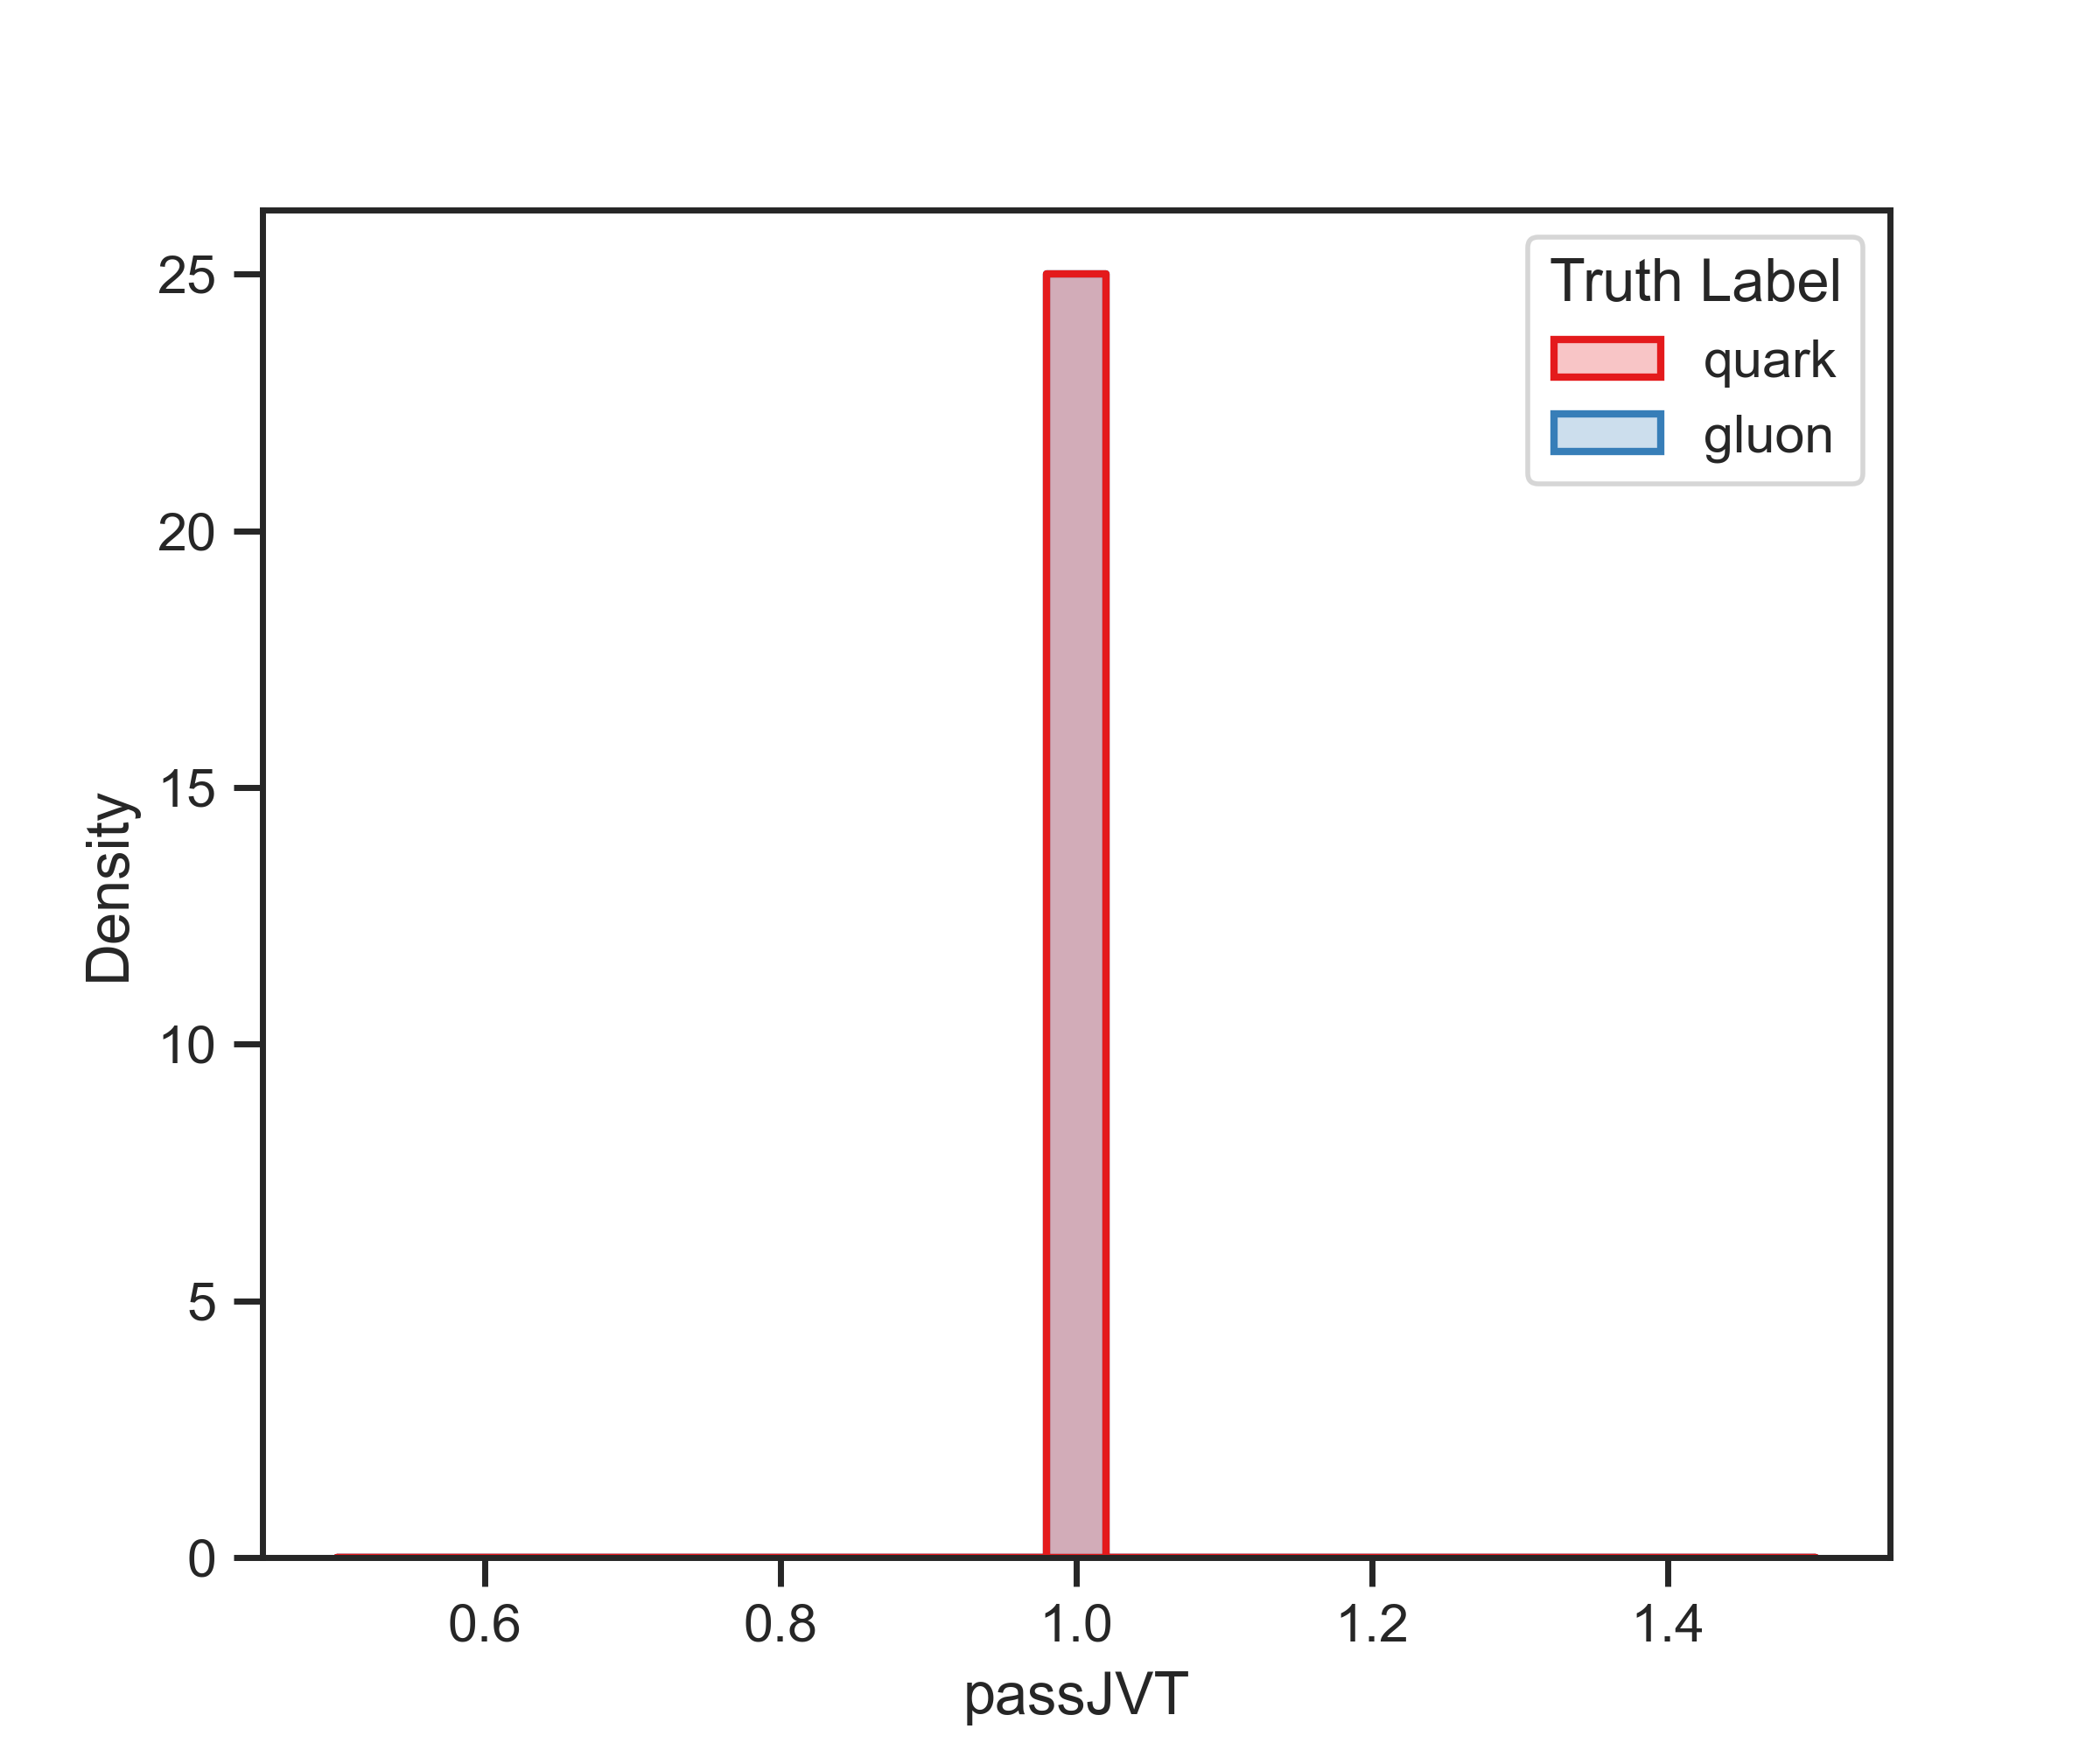
\includegraphics[width=1\textwidth]{src/plots/distributions/highlevel/jets_passJVT.png}
		\caption{\texttt{jets\_passJVT}}
		\label{fig:highlevel_27}
	\end{subfigure}
	\begin{subfigure}[t]{0.49\textwidth}
		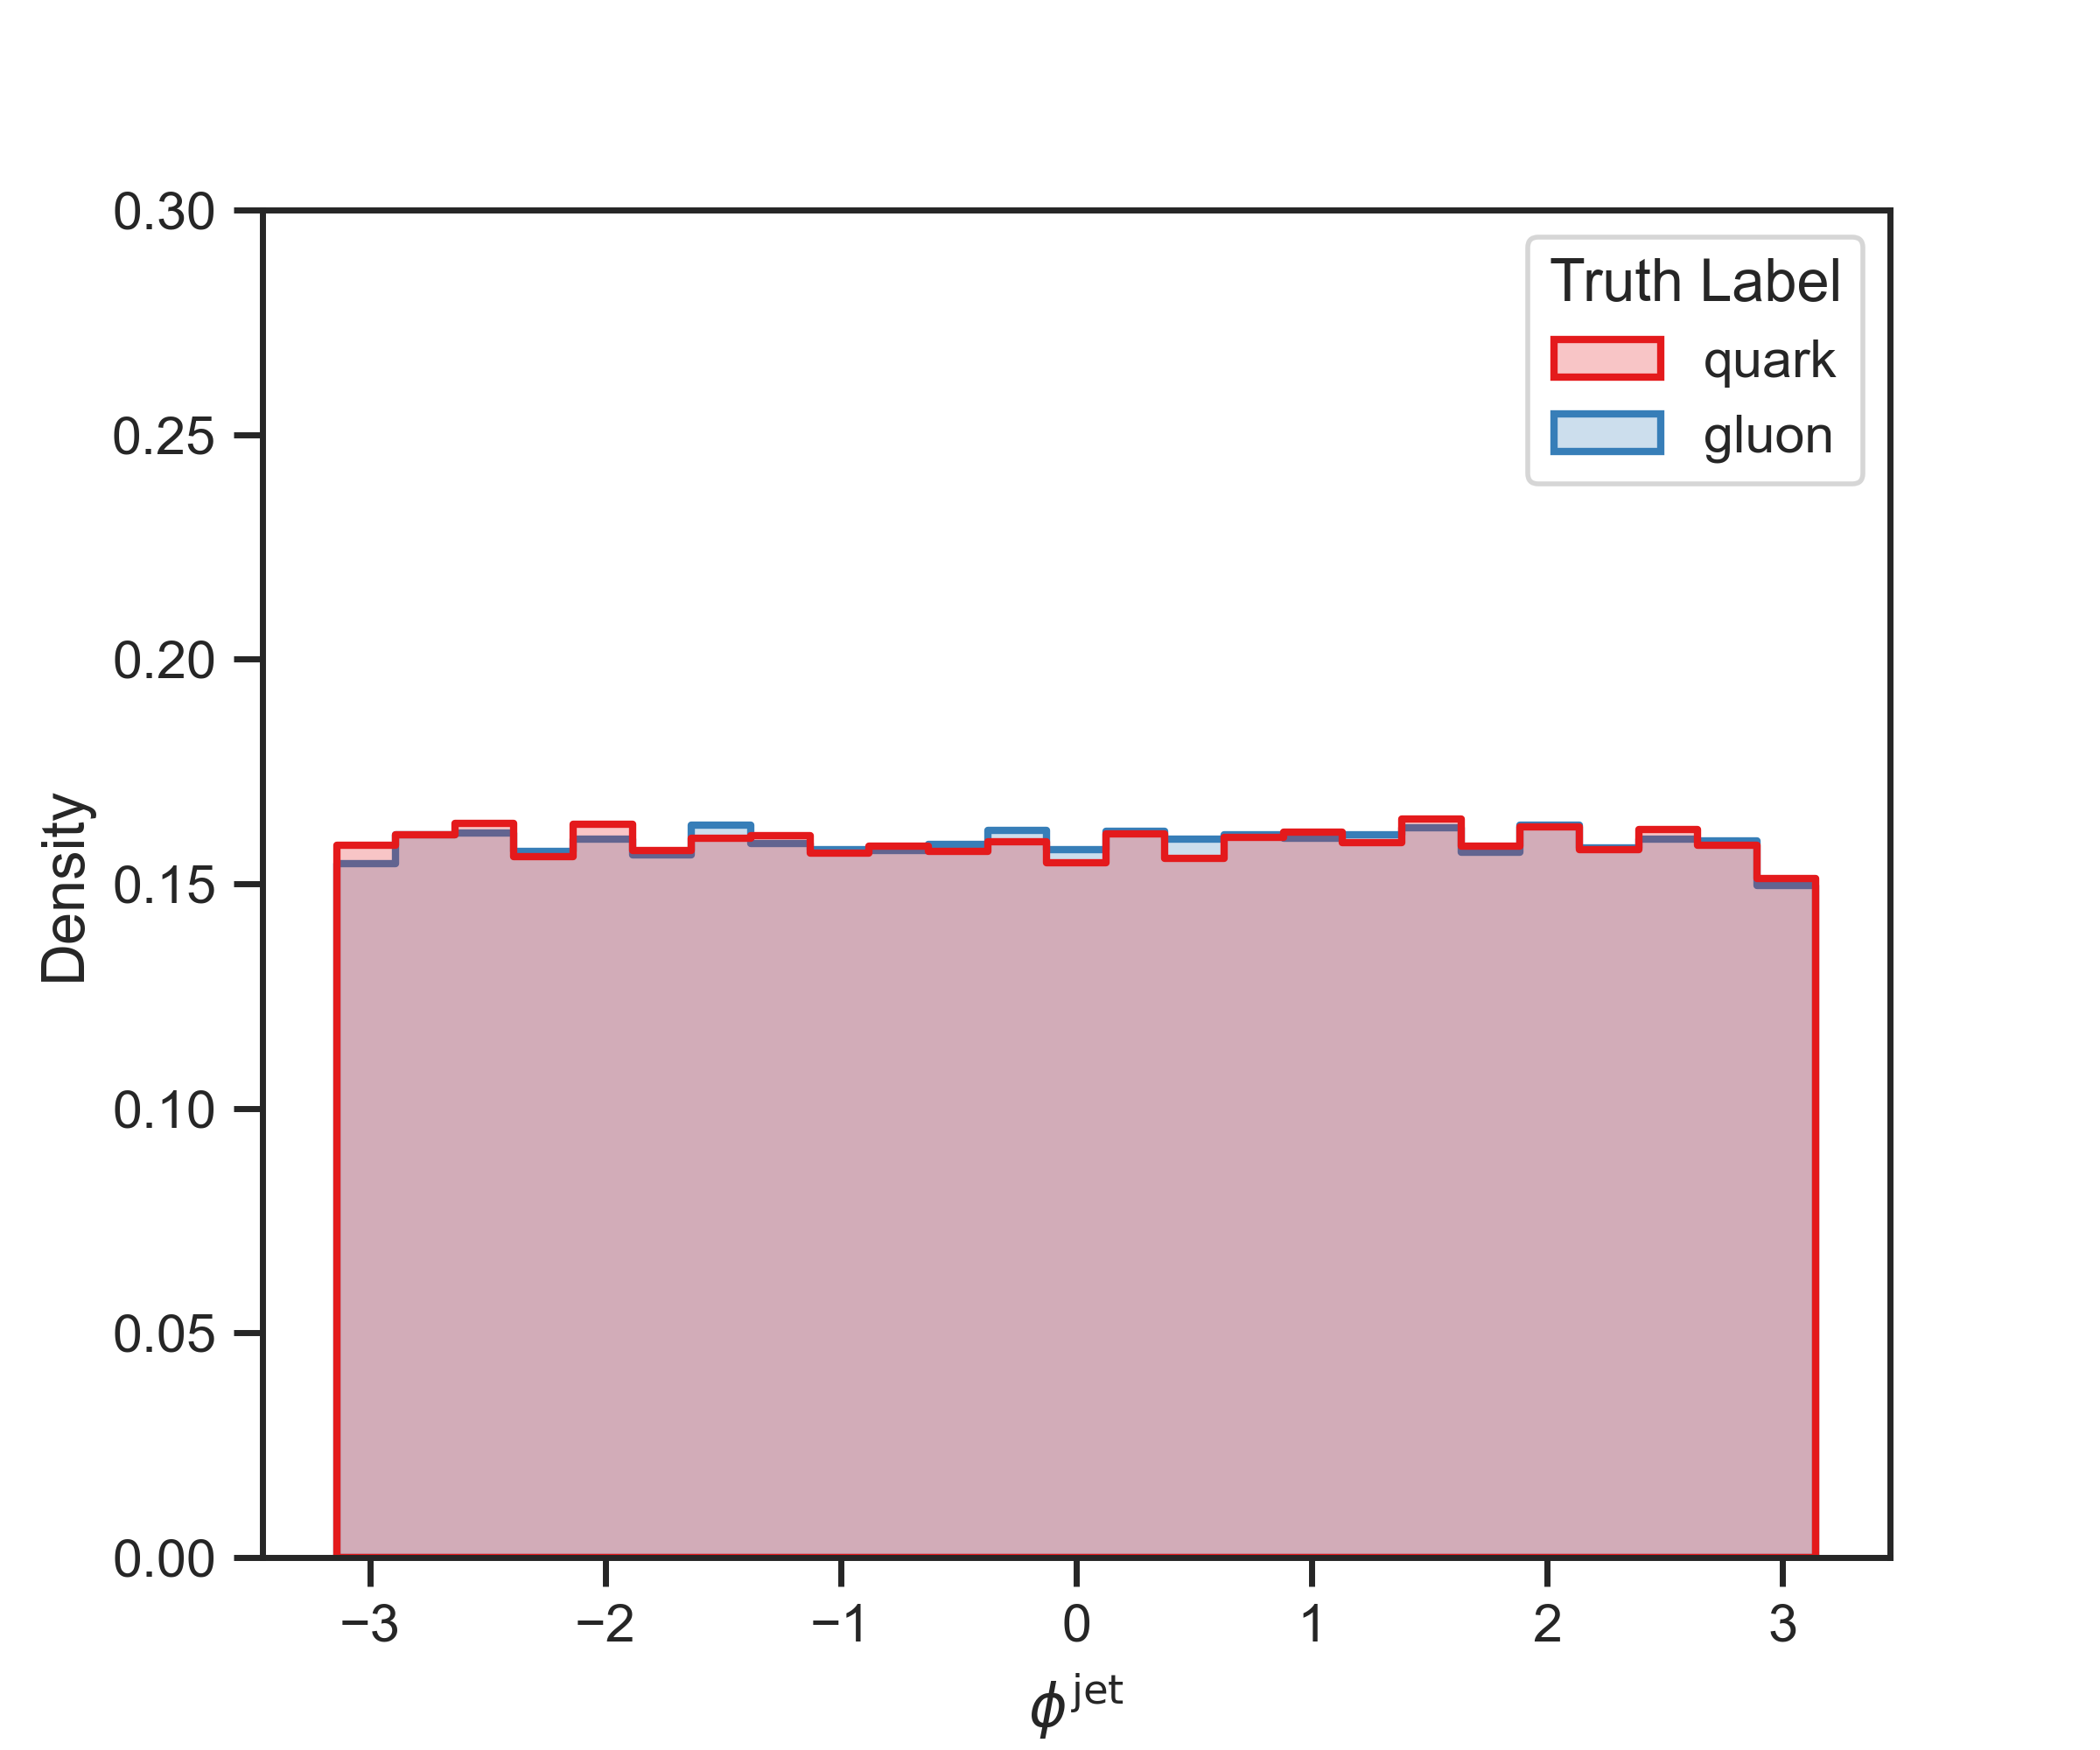
\includegraphics[width=1\textwidth]{src/plots/distributions/highlevel/jets_phi.png}
		\caption{\texttt{jets\_phi}}
		\label{fig:highlevel_28}
	\end{subfigure}
	\begin{subfigure}[t]{0.49\textwidth}
		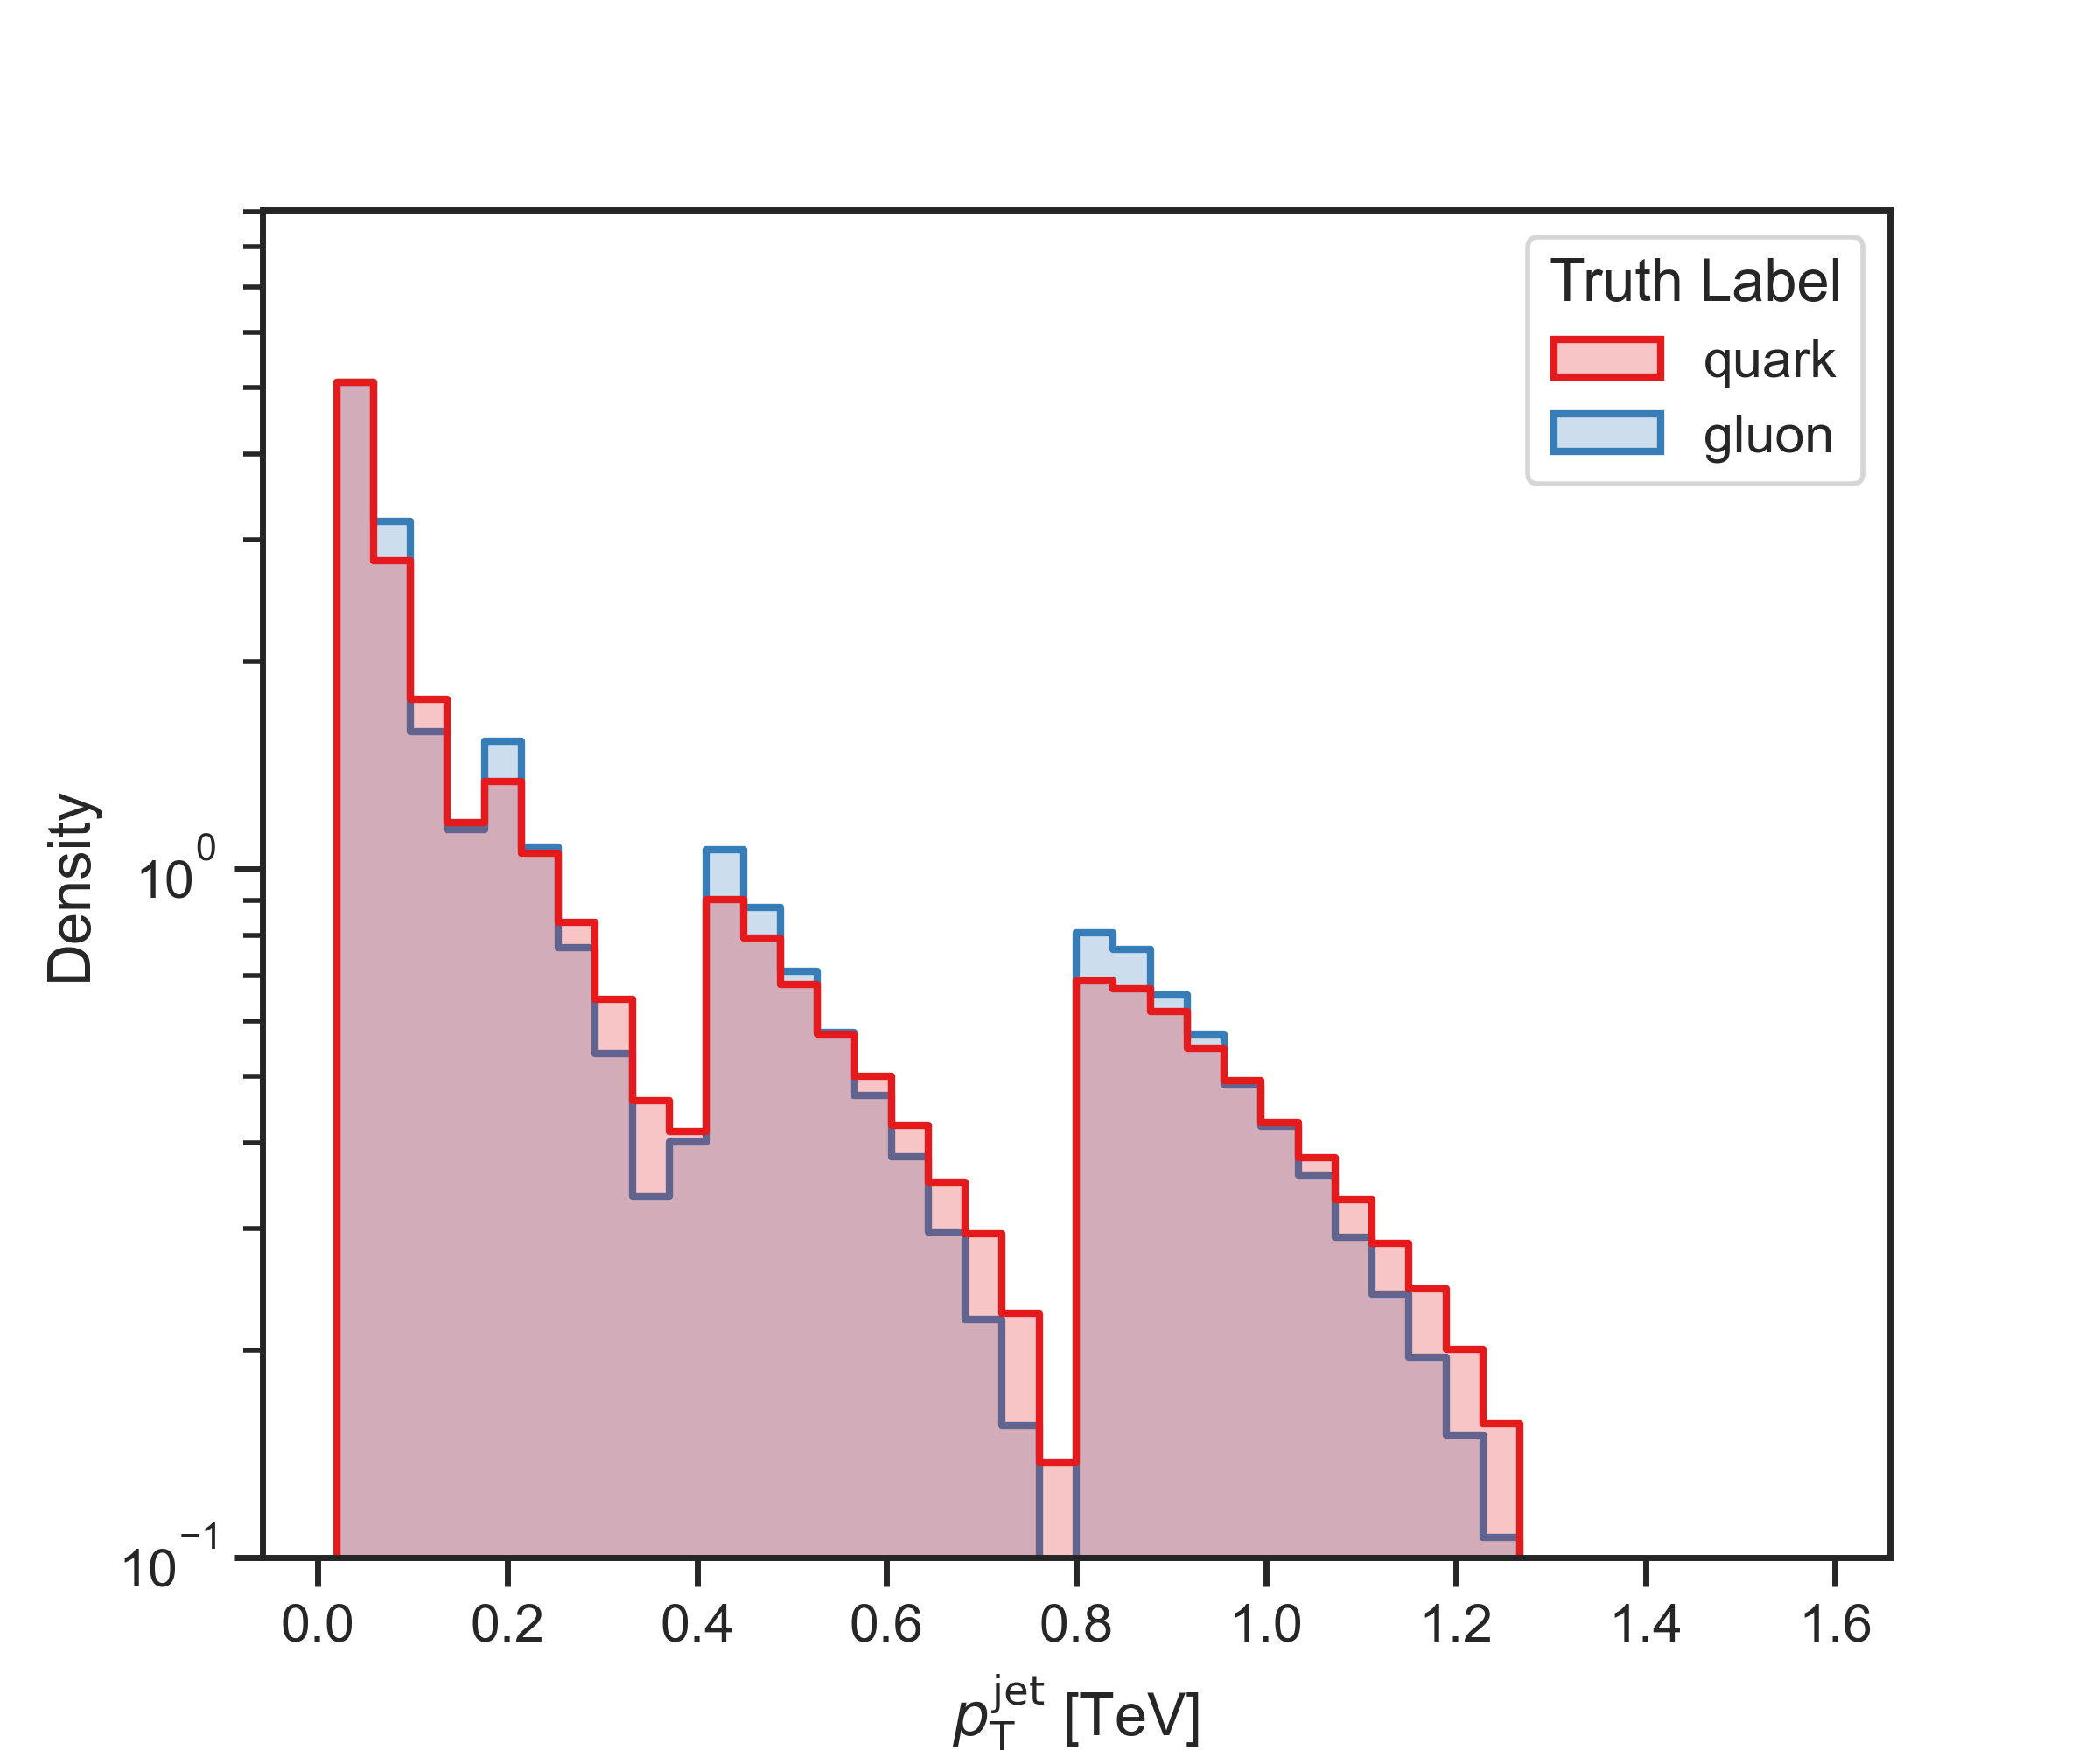
\includegraphics[width=1\textwidth]{src/plots/distributions/highlevel/jets_pt.png}
		\caption{\texttt{jets\_pt}}
		\label{fig:highlevel_29}
	\end{subfigure}
\caption{High-level Jet Variables, part 5}
\label{fig:highlevel_24-29}
\end{figure}

